\documentclass[12pt,journal,onecolumn,final]{IEEEtran}
%
% If IEEEtran.cls has not been installed into the LaTeX system files,
% manually specify the path to it like:
% \documentclass[journal]{../sty/IEEEtran}




% Some very useful LaTeX packages include:
% (uncomment the ones you want to load)


% *** MISC UTILITY PACKAGES ***
%
%\usepackage{ifpdf}
% Heiko Oberdiek's ifpdf.sty is very useful if you need conditional
% compilation based on whether the output is pdf or dvi.
% usage:
% \ifpdf
%   % pdf code
% \else
%   % dvi code
% \fi
% The latest version of ifpdf.sty can be obtained from:
% http://www.ctan.org/pkg/ifpdf
% Also, note that IEEEtran.cls V1.7 and later provides a builtin
% \ifCLASSINFOpdf conditional that works the same way.
% When switching from latex to pdflatex and vice-versa, the compiler may
% have to be run twice to clear warning/error messages.






% *** CITATION PACKAGES ***
%
\usepackage{cite}
% cite.sty was written by Donald Arseneau
% V1.6 and later of IEEEtran pre-defines the format of the cite.sty package
% \cite{} output to follow that of the IEEE. Loading the cite package will
% result in citation numbers being automatically sorted and properly
% "compressed/ranged". e.g., [1], [9], [2], [7], [5], [6] without using
% cite.sty will become [1], [2], [5]--[7], [9] using cite.sty. cite.sty's
% \cite will automatically add leading space, if needed. Use cite.sty's
% noadjust option (cite.sty V3.8 and later) if you want to turn this off
% such as if a citation ever needs to be enclosed in parenthesis.
% cite.sty is already installed on most LaTeX systems. Be sure and use
% version 5.0 (2009-03-20) and later if using hyperref.sty.
% The latest version can be obtained at:
% http://www.ctan.org/pkg/cite
% The documentation is contained in the cite.sty file itself.






% *** GRAPHICS RELATED PACKAGES ***
%
\ifCLASSINFOpdf
  \usepackage[pdftex]{graphicx}
  % declare the path(s) where your graphic files are
  % \graphicspath{{../pdf/}{../jpeg/}}
  % and their extensions so you won't have to specify these with
  % every instance of \includegraphics
  % \DeclareGraphicsExtensions{.pdf,.jpeg,.png}
\else
  % or other class option (dvipsone, dvipdf, if not using dvips). graphicx
  % will default to the driver specified in the system graphics.cfg if no
  % driver is specified.
  \usepackage[dvips]{graphicx}
  % declare the path(s) where your graphic files are
  % \graphicspath{{../eps/}}
  % and their extensions so you won't have to specify these with
  % every instance of \includegraphics
  % \DeclareGraphicsExtensions{.eps}
\fi
% graphicx was written by David Carlisle and Sebastian Rahtz. It is
% required if you want graphics, photos, etc. graphicx.sty is already
% installed on most LaTeX systems. The latest version and documentation
% can be obtained at:
% http://www.ctan.org/pkg/graphicx
% Another good source of documentation is "Using Imported Graphics in
% LaTeX2e" by Keith Reckdahl which can be found at:
% http://www.ctan.org/pkg/epslatex
%
% latex, and pdflatex in dvi mode, support graphics in encapsulated
% postscript (.eps) format. pdflatex in pdf mode supports graphics
% in .pdf, .jpeg, .png and .mps (metapost) formats. Users should ensure
% that all non-photo figures use a vector format (.eps, .pdf, .mps) and
% not a bitmapped formats (.jpeg, .png). The IEEE frowns on bitmapped formats
% which can result in "jaggedy"/blurry rendering of lines and letters as
% well as large increases in file sizes.
%
% You can find documentation about the pdfTeX application at:
% http://www.tug.org/applications/pdftex





% *** MATH PACKAGES ***
%
\usepackage{amsmath}
% A popular package from the American Mathematical Society that provides
% many useful and powerful commands for dealing with mathematics.
%
% Note that the amsmath package sets \interdisplaylinepenalty to 10000
% thus preventing page breaks from occurring within multiline equations. Use:
%\interdisplaylinepenalty=2500
% after loading amsmath to restore such page breaks as IEEEtran.cls normally
% does. amsmath.sty is already installed on most LaTeX systems. The latest
% version and documentation can be obtained at:
% http://www.ctan.org/pkg/amsmath





% *** SPECIALIZED LIST PACKAGES ***
%
%\usepackage{algorithmic}
% algorithmic.sty was written by Peter Williams and Rogerio Brito.
% This package provides an algorithmic environment fo describing algorithms.
% You can use the algorithmic environment in-text or within a figure
% environment to provide for a floating algorithm. Do NOT use the algorithm
% floating environment provided by algorithm.sty (by the same authors) or
% algorithm2e.sty (by Christophe Fiorio) as the IEEE does not use dedicated
% algorithm float types and packages that provide these will not provide
% correct IEEE style captions. The latest version and documentation of
% algorithmic.sty can be obtained at:
% http://www.ctan.org/pkg/algorithms
% Also of interest may be the (relatively newer and more customizable)
% algorithmicx.sty package by Szasz Janos:
% http://www.ctan.org/pkg/algorithmicx




% *** ALIGNMENT PACKAGES ***
%
\usepackage{array}
% Frank Mittelbach's and David Carlisle's array.sty patches and improves
% the standard LaTeX2e array and tabular environments to provide better
% appearance and additional user controls. As the default LaTeX2e table
% generation code is lacking to the point of almost being broken with
% respect to the quality of the end results, all users are strongly
% advised to use an enhanced (at the very least that provided by array.sty)
% set of table tools. array.sty is already installed on most systems. The
% latest version and documentation can be obtained at:
% http://www.ctan.org/pkg/array


% IEEEtran contains the IEEEeqnarray family of commands that can be used to
% generate multiline equations as well as matrices, tables, etc., of high
% quality.




% *** SUBFIGURE PACKAGES ***
\ifCLASSOPTIONcompsoc
  \usepackage[caption=false,font=normalsize,labelfont=sf,textfont=sf]{subfig}
\else
  \usepackage[caption=false,font=footnotesize]{subfig}
\fi
% subfig.sty, written by Steven Douglas Cochran, is the modern replacement
% for subfigure.sty, the latter of which is no longer maintained and is
% incompatible with some LaTeX packages including fixltx2e. However,
% subfig.sty requires and automatically loads Axel Sommerfeldt's caption.sty
% which will override IEEEtran.cls' handling of captions and this will result
% in non-IEEE style figure/table captions. To prevent this problem, be sure
% and invoke subfig.sty's "caption=false" package option (available since
% subfig.sty version 1.3, 2005/06/28) as this is will preserve IEEEtran.cls
% handling of captions.
% Note that the Computer Society format requires a larger sans serif font
% than the serif footnote size font used in traditional IEEE formatting
% and thus the need to invoke different subfig.sty package options depending
% on whether compsoc mode has been enabled.
%
% The latest version and documentation of subfig.sty can be obtained at:
% http://www.ctan.org/pkg/subfig




% *** FLOAT PACKAGES ***
%
%\usepackage{fixltx2e}
% fixltx2e, the successor to the earlier fix2col.sty, was written by
% Frank Mittelbach and David Carlisle. This package corrects a few problems
% in the LaTeX2e kernel, the most notable of which is that in current
% LaTeX2e releases, the ordering of single and double column floats is not
% guaranteed to be preserved. Thus, an unpatched LaTeX2e can allow a
% single column figure to be placed prior to an earlier double column
% figure.
% Be aware that LaTeX2e kernels dated 2015 and later have fixltx2e.sty's
% corrections already built into the system in which case a warning will
% be issued if an attempt is made to load fixltx2e.sty as it is no longer
% needed.
% The latest version and documentation can be found at:
% http://www.ctan.org/pkg/fixltx2e


%\usepackage{stfloats}
% stfloats.sty was written by Sigitas Tolusis. This package gives LaTeX2e
% the ability to do double column floats at the bottom of the page as well
% as the top. (e.g., "\begin{figure*}[!b]" is not normally possible in
% LaTeX2e). It also provides a command:
%\fnbelowfloat
% to enable the placement of footnotes below bottom floats (the standard
% LaTeX2e kernel puts them above bottom floats). This is an invasive package
% which rewrites many portions of the LaTeX2e float routines. It may not work
% with other packages that modify the LaTeX2e float routines. The latest
% version and documentation can be obtained at:
% http://www.ctan.org/pkg/stfloats
% Do not use the stfloats baselinefloat ability as the IEEE does not allow
% \baselineskip to stretch. Authors submitting work to the IEEE should note
% that the IEEE rarely uses double column equations and that authors should try
% to avoid such use. Do not be tempted to use the cuted.sty or midfloat.sty
% packages (also by Sigitas Tolusis) as the IEEE does not format its papers in
% such ways.
% Do not attempt to use stfloats with fixltx2e as they are incompatible.
% Instead, use Morten Hogholm'a dblfloatfix which combines the features
% of both fixltx2e and stfloats:
%
% \usepackage{dblfloatfix}
% The latest version can be found at:
% http://www.ctan.org/pkg/dblfloatfix




%\ifCLASSOPTIONcaptionsoff
%  \usepackage[nomarkers]{endfloat}
% \let\MYoriglatexcaption\caption
% \renewcommand{\caption}[2][\relax]{\MYoriglatexcaption[#2]{#2}}
%\fi
% endfloat.sty was written by James Darrell McCauley, Jeff Goldberg and
% Axel Sommerfeldt. This package may be useful when used in conjunction with
% IEEEtran.cls'  captionsoff option. Some IEEE journals/societies require that
% submissions have lists of figures/tables at the end of the paper and that
% figures/tables without any captions are placed on a page by themselves at
% the end of the document. If needed, the draftcls IEEEtran class option or
% \CLASSINPUTbaselinestretch interface can be used to increase the line
% spacing as well. Be sure and use the nomarkers option of endfloat to
% prevent endfloat from "marking" where the figures would have been placed
% in the text. The two hack lines of code above are a slight modification of
% that suggested by in the endfloat docs (section 8.4.1) to ensure that
% the full captions always appear in the list of figures/tables - even if
% the user used the short optional argument of \caption[]{}.
% IEEE papers do not typically make use of \caption[]'s optional argument,
% so this should not be an issue. A similar trick can be used to disable
% captions of packages such as subfig.sty that lack options to turn off
% the subcaptions:
% For subfig.sty:
% \let\MYorigsubfloat\subfloat
% \renewcommand{\subfloat}[2][\relax]{\MYorigsubfloat[]{#2}}
% However, the above trick will not work if both optional arguments of
% the \subfloat command are used. Furthermore, there needs to be a
% description of each subfigure *somewhere* and endfloat does not add
% subfigure captions to its list of figures. Thus, the best approach is to
% avoid the use of subfigure captions (many IEEE journals avoid them anyway)
% and instead reference/explain all the subfigures within the main caption.
% The latest version of endfloat.sty and its documentation can obtained at:
% http://www.ctan.org/pkg/endfloat
%
% The IEEEtran \ifCLASSOPTIONcaptionsoff conditional can also be used
% later in the document, say, to conditionally put the References on a
% page by themselves.




% *** PDF, URL AND HYPERLINK PACKAGES ***
%
%\usepackage{url}
% url.sty was written by Donald Arseneau. It provides better support for
% handling and breaking URLs. url.sty is already installed on most LaTeX
% systems. The latest version and documentation can be obtained at:
% http://www.ctan.org/pkg/url
% Basically, \url{my_url_here}.




% *** Do not adjust lengths that control margins, column widths, etc. ***
% *** Do not use packages that alter fonts (such as pslatex).         ***
% There should be no need to do such things with IEEEtran.cls V1.6 and later.
% (Unless specifically asked to do so by the journal or conference you plan
% to submit to, of course. )

\usepackage{transparent}
\usepackage{acro}
\usepackage{siunitx}
\usepackage{longtable,booktabs}
\usepackage{threeparttable}
\usepackage{multirow}
\usepackage{colortbl}
\usepackage{tabularx}
\usepackage{arydshln}
\usepackage{pdflscape}
\usepackage{ltxtable}
\usepackage{pifont}
\usepackage{color}
\usepackage{tikz,xifthen}
\usepackage{tikz-qtree}
\usepackage[numbers]{natbib}
\let\labelindent\relax
\usepackage{enumitem}
\usepackage{amssymb}

\definecolor{codegreen}{rgb}{0,0.6,0}
\definecolor{codegray}{rgb}{0.5,0.5,0.5}
\definecolor{codepurple}{rgb}{0.58,0,0.82}
\definecolor{backcolour}{rgb}{0.95,0.95,0.92}

\newcommand{\cmark}{\color{green!60!black!80}\ding{51}}
\newcommand{\mmark}{{\color{green!60!black!80}\ding{51}}$^{!}$}
\newcommand{\xmark}{\color{red!60!black!80}\ding{55}}
\newcommand{\cmarksmall}{\color{green!60!black!80}\ding{51}}
\newcommand{\mmarksmall}{{\color{green!60!black!80}\ding{51}}$^{!}$}
\newcommand{\xmarksmall}{\color{red!60!black!80}\ding{55}}
\newcommand{\Conv}{\mathop{\scalebox{1.5}{\raisebox{-0.2ex}{$\ast$}}}}

\definecolor{autoGuided}{rgb}{ 0.3765    0.7294    0.9412}
\newcommand{\autoGuidedColor}{(light-Blue)}
\definecolor{fullyAuto}{rgb}{ 0.0941    0.3843    0.6627}
\newcommand{\fullyAutoColor}{(dark-blue)}
\definecolor{semiAuto}{rgb}{ 0.0784    0.5059    0.1686}
\newcommand{\semiAutoColor}{(light-green)}
\definecolor{fullyGuided}{rgb}{ 0.4275    0.6902    0.3176}
\newcommand{\fullyGuidedColor}{(dark-green)}

\usetikzlibrary{decorations.pathmorphing}
\usetikzlibrary{fit}
\usetikzlibrary{backgrounds}
\usetikzlibrary{shapes,arrows,shadows}
\usetikzlibrary{calc,decorations.pathreplacing,decorations.markings,positioning}
\usetikzlibrary{snakes,decorations.text,shapes,patterns}

\DeclareMathOperator*{\argmin}{arg\,min}
\DeclareMathOperator*{\argmax}{arg\,max}
\DeclareMathOperator*{\sign}{sign}
\DeclareMathOperator*{\infspie}{inf}

%\usepackage[table]{xcolor}
%% The amssymb package provides various useful mathematical symbols
\usepackage{amssymb}

%% The amsthm package provides extended theorem environments
\usepackage{amsthm}

%% amsmath for math environment
\usepackage{amsmath}

\DeclareMathOperator*{\argmin}{arg\,min}
\DeclareMathOperator*{\argmax}{arg\,max}
\DeclareMathOperator*{\sign}{sign}
\DeclareMathOperator*{\infspie}{inf}


% to break equation
%\usepackage{mathpazo}
%\usepackage{mathptmx}
%\usepackage[mathpazo]{flexisym}
%\usepackage{breqn}

%% For clever reference
%\usepackage{cleveref}

%% color package
\usepackage{color}

%% figure package
\usepackage{epsf,graphicx}
\usepackage{epstopdf}
%\usepackage{subfigure}
\usepackage{transparent}

%% New environment to have some indent inside enumerate environment
\usepackage{enumitem}

%% To create acronym for proper glossary
\usepackage{acro}

%% To number the line in the article
\usepackage{lineno}

%% Environment to include table with notes
\usepackage{array}
\usepackage{threeparttable}
\usepackage{booktabs}
\usepackage{multirow}
\usepackage{siunitx}

%% In order to change size of margin
\usepackage{geometry}
\usepackage{changepage}
\usepackage{lscape}
%% Colorpackage for table
\usepackage{colortbl}
\usepackage{tabularx}
\usepackage{arydshln}

%% To use URL referencing
\usepackage{url}
%\usepackage[hidelinks]{hyperref}

%% In order to draw some graphs
\usepackage{tikz,xifthen}
\usepackage{tikz-qtree}
\usetikzlibrary{decorations.pathmorphing} % noisy shapes
\usetikzlibrary{fit}					% fitting shapes to coordinates
\usetikzlibrary{backgrounds}	% drawing the background after the foreground
\usetikzlibrary{shapes,arrows,shadows}
\usetikzlibrary{calc,decorations.pathreplacing,decorations.markings,positioning}
\usetikzlibrary{snakes,decorations.text,shapes,patterns}
%\usepackage{scalefnt,lmodern,booktabs}

%% Paxkage for cross and tick symbols
\usepackage{pifont}
\newcommand{\cmark}{\color{green!60!black!80}\ding{51}}
\newcommand{\mmark}{{\color{green!60!black!80}\ding{51}}$^{!}$}
\newcommand{\xmark}{\color{red!60!black!80}\ding{55}}
\newcommand{\cmarksmall}{\color{green!60!black!80}\ding{51}}
\newcommand{\mmarksmall}{{\color{green!60!black!80}\ding{51}}$^{!}$}
\newcommand{\xmarksmall}{\color{red!60!black!80}\ding{55}}
\newcommand{\Conv}{\mathop{\scalebox{1.5}{\raisebox{-0.2ex}{$\ast$}}}}%

\definecolor{autoGuided}{rgb}{ 0.3765    0.7294    0.9412}
\newcommand{\autoGuidedColor}{(light-Blue)}
\definecolor{fullyAuto}{rgb}{ 0.0941    0.3843    0.6627}
\newcommand{\fullyAutoColor}{(dark-blue)}
\definecolor{semiAuto}{rgb}{ 0.0784    0.5059    0.1686}
\newcommand{\semiAutoColor}{(light-green)}
\definecolor{fullyGuided}{rgb}{ 0.4275    0.6902    0.3176}
\newcommand{\fullyGuidedColor}{(dark-green)}

\DeclareSIUnit\ppm{ppm}
\DeclareSIUnit\px{px}

\usepackage{ltxtable}
\usepackage{listings}
\usepackage{color}
% \usepackage[toc]{appendix}

\definecolor{codegreen}{rgb}{0,0.6,0}
\definecolor{codegray}{rgb}{0.5,0.5,0.5}
\definecolor{codepurple}{rgb}{0.58,0,0.82}
\definecolor{backcolour}{rgb}{0.95,0.95,0.92}

\lstdefinestyle{mystyle}{
    backgroundcolor=\color{backcolour},
    commentstyle=\color{codegreen},
    keywordstyle=\color{magenta},
    numberstyle=\tiny\color{codegray},
    stringstyle=\color{codepurple},
    basicstyle=\footnotesize,
    breakatwhitespace=false,
    breaklines=true,
    captionpos=b,
    keepspaces=true,
    numbers=left,
    numbersep=5pt,
    showspaces=false,
    showstringspaces=false,
    showtabs=false,
    tabsize=2
}

\lstset{style=mystyle}
\usepackage{setspace}

\usepackage[numbers]{natbib}

%\acrodef{cap}[CaP]{prostate cancer}
\DeclareAcronym{cap}{
short = CaP,
long = prostate cancer
}
%\acrodef{cade}[CADe]{computer-aided detection}
\DeclareAcronym{cade}{
short = CADe,
long = computer-aided detection
}
%\acrodef{cadx}[CADx]{computer-aided diagnosis}
\DeclareAcronym{cadx}{
short = CADx,
long = computer-aided diagnosis
}
\DeclareAcronym{lm}{
short = LM,
long = Leung-Malik set
}
%\acrodef{us}[US]{ultrasound}
\DeclareAcronym{us}{
short = UTS,
long = ultrasound
}
%\acrodef{ct}[CT]{computer tomography}
\DeclareAcronym{ct}{
short = CT,
long = computer tomography
}
%\acrodef{cad}[CAD]{computer-aided detection and diagnosis}
\DeclareAcronym{cad}{
short = CAD,
long = computer-aided detection and diagnosis
}
%\acrodef{mri}[MRI]{magnetic resonance imaging}
\DeclareAcronym{mri}{
short = MRI,
long = magnetic resonance imaging
}
%\acrodef{nmr}[NMR]{nuclear magnetic resonance}
\DeclareAcronym{nmr}{
short = NMR,
long = nuclear magnetic resonance
}

\DeclareAcronym{omp}{
  short = OMP,
  long =  orthogonal matching pursuit
}
\DeclareAcronym{adb}{
  short = AdB,
  long = AdaBoost
}
\DeclareAcronym{gb}{
  short = GB,
  long = Gradient Boosting
}

\DeclareAcronym{mp}{
  short = MP,
  long =  Matching Pursuit
}
%\acrodef{t2w}[T$_2$-W]{T$_2$ Weighted}
\DeclareAcronym{t2w}{
short = T$_2$-W,
long = T$_2$ Weighted
}
%\acrodef{dce}[DCE]{dynamic contrast-enhanced}
\DeclareAcronym{dce}{
short = DCE,
long = dynamic contrast-enhanced
}
%\acrodef{dw}[DW]{diffusion weighted}
\DeclareAcronym{dw}{
short = DW,
long = diffusion weighted
}
%\acrodef{mrsi}[MRSI]{magnetic resonance spectroscopy imaging}
\DeclareAcronym{mrsi}{
short = MRSI,
long = magnetic resonance spectroscopy imaging
}
%\acrodef{bph}[BPH]{benign prostatic hyperplasia}
\DeclareAcronym{bph}{
short = BPH,
long = benign prostatic hyperplasia
}
%\acrodef{pz}[PZ]{peripheral zone}
\DeclareAcronym{pz}{
short = PZ,
long = peripheral zone
}
%\acrodef{cz}[CZ]{central zone}

\DeclareAcronym{mpmri}{
short = mp-MRI,
long = multiparametric \ac{mri}
}
\DeclareAcronym{cz}{
short = CZ,
long = central zone
}
%\acrodef{tz}[TZ]{transitional zone}
\DeclareAcronym{tz}{
short = TZ,
long = transitional zone
}
%\acrodef{cg}[CG]{central gland}
\DeclareAcronym{cg}{
short = CG,
long = central gland
}
%\acrodef{psa}[PSA]{prostate-specific antigen}
\DeclareAcronym{psa}{
short = PSA,
long = prostate-specific antigen
}
%\acrodef{trus}[TRUS]{transrectal ultrasound}
\DeclareAcronym{trus}{
short = TRUS,
long = transrectal ultrasound
}
%\acrodef{tr}[TR]{repetition time}
\DeclareAcronym{tr}{
short = TR,
long = repetition time
}
%\acrodef{te}[TE]{echo time}
\DeclareAcronym{te}{
short = TE,
long = echo time
}
%\acrodef{si}[SI]{signal intensity}
\DeclareAcronym{si}{
short = SI,
long = signal intensity
}
%\acrodef{ees}[EES]{extravascular-extracellular space}
\DeclareAcronym{ees}{
short = EES,
long = extravascular-extracellular space
}
%\acrodef{t1w}[T$_1$-W]{T$_1$ Weighted}
\DeclareAcronym{t1w}{
short = T$_1$-W,
long = T$_1$ Weighted
}
%\acrodef{fse}[FSE]{Fast Spin-Echo}
\DeclareAcronym{fse}{
short = FSE,
long = Fast Spin-Echo
}
%\acrodef{adc}[ADC]{Apparent Diffusion Coeffient}
\DeclareAcronym{adc}{
short = ADC,
long = apparent diffusion coefficient
}
%\acrodef{roi}[ROI]{region of interest}
\DeclareAcronym{roi}{
short = ROI,
long = region of interest
}
%\acrodef{cse}[CSE]{chemical shift effect}
\DeclareAcronym{cse}{
short = CSE,
long = chemical shift effect
}
%\acrodef{snr}[SNR]{signal-to-noise}
\DeclareAcronym{snr}{
short = SNR,
long = signal-to-noise
}
\DeclareAcronym{se}{
short = SE,
long = sensitivity
}
\DeclareAcronym{sp}{
short = SP,
long = specificity
}
%\acrodef{gs}[GS]{Gleason score}
\DeclareAcronym{gs}{
short = GS,
long = Gleason score
}
%\acrodef{ersspc}[ERSSPC]{European Randomized Study of Screening for Prostate Cancer}
\DeclareAcronym{ersspc}{
short = ERSSPC,
long = European randomized study of screening for prostate cancer
}
%\acrodef{plco}[PLCO]{Prostate, Lung, Colorectal and Ovarian}
\DeclareAcronym{plco}{
short = PLCO,
long = prostate lung colorectal and ovarian
}
%\acrodef{fig}[Fig.]{figure}
\DeclareAcronym{fig}{
short = Fig.,
long = figure,
class = latex
}
\DeclareAcronym{tab}{
short = Table,
long = table,
class = latex
}
\DeclareAcronym{eq}{
short = Eq.,
long = equation,
class = latex
}
\DeclareAcronym{sec}{
short = Sect.,
long = section,
class = latex
}
\DeclareAcronym{chp}{
short = Sect.,
long = Section,
class = latex
}

\DeclareAcronym{fov}{
short = FOV,
long = field of view
}
\DeclareAcronym{dwt}{
short = DWT,
long = discrete wavelet transform
}
\DeclareAcronym{dwst}{
short = DWST,
long = discrete wavelet squared transform
}
\DeclareAcronym{map}{
short = MAP,
long = maximum \textit{a posteriori}
}
\DeclareAcronym{ml}{
short = ML,
long = maximum likelihood
}
\DeclareAcronym{mle}{
short = MLE,
long = maximum likelihood estimation
}
\DeclareAcronym{mrf}{
short = MRF,
long = Markov random field
}
\DeclareAcronym{itk}{
short = ITK,
long = Insight Segmentation and Registration Toolkit
}
\DeclareAcronym{es}{
short = ES,
long = Evolution Strategy
}
\DeclareAcronym{scf}{
short = SCF,
long = sparse coded features
}
\DeclareAcronym{bow}{
short = BoW,
long = bag of words
}
\DeclareAcronym{pdf}{
short = PDF,
long = probability density function
}
\DeclareAcronym{gscale}{
short = \textit{g}-scale,
long = generalized scale
}
\DeclareAcronym{aif}{
short = AIF,
long = arterial input function
}
\DeclareAcronym{svd}{
short = SVD,
long = singular value decomposition
}
\DeclareAcronym{mse}{
short = MSE,
long = mean squared error
}
\DeclareAcronym{mi}{
short = MI,
long = mutual information
}
\DeclareAcronym{mantra}{
short = MANTRA,
long = multi-attribute non-initializing texture reconstruction based active shape model
}
\DeclareAcronym{asm}{
short = ASM,
long = active shape model
}
\DeclareAcronym{pca}{
short = PCA,
long = principal components analysis
}
\DeclareAcronym{weritas}{
short = WERITAS,
long = weighted ensemble of regional image textures for active shape model segmentation
}
\DeclareAcronym{staple}{
short = STAPLE,
long = simultaneous truth and performance level estimation
}
\DeclareAcronym{lda}{
short = LDA,
long = linear discriminant analysis
}
\DeclareAcronym{lbp}{
short = LBP,
long = local binary pattern
}
\DeclareAcronym{tps}{
short = TPS,
long = thin plate spline
}
\DeclareAcronym{acm}{
short = ACM,
long = active contour model
}
\DeclareAcronym{cmi}{
short = CMI,
long = combined mutual information
}
\DeclareAcronym{svm}{
short = SVM,
long = support vector machines
}
\DeclareAcronym{rvm}{
short = RVM,
long = relevant vector machine
}
\DeclareAcronym{rbf}{
short = RBF,
long = radial basis function
}
\DeclareAcronym{knn}{
short = $k$-NN,
long = $k$-nearest neighbour
}
\DeclareAcronym{nn}{
short = NN,
long = neareast neighbour
}
\DeclareAcronym{dct}{
short = DCT,
long = discrete cosine transform
}
\DeclareAcronym{hog}{
short = HOG,
long = histogram of oriented gradient
}
\DeclareAcronym{dft}{
short = DFT,
long = discrete fourier transform
}
\DeclareAcronym{us1}{
short = US,
long = under-sampling
}
\DeclareAcronym{os}{
short = OS,
long = over-sampling
}
\DeclareAcronym{ros}{
short = ROS,
long = random-over-sampling
}
\DeclareAcronym{rus}{
short = RUS,
long = random-under-sampling
}
\DeclareAcronym{nm}{
short = NM,
long = nearmiss
}
\DeclareAcronym{nm3}{
short = NM-3,
long = nearmiss-3
}
\DeclareAcronym{nm2}{
short = NM-2,
long = nearmiss-2
}
\DeclareAcronym{nm1}{
short = NM-1,
long = nearmiss-1
}
\DeclareAcronym{iht}{
short = IHT,
long = instance-hardness-threshold
}
\DeclareAcronym{smote}{
short = SMOTE,
long = synthetic minority over-sampling techniques
}
\DeclareAcronym{smoteb1}{
short = SMOTE-b1,
long = SMOTE-borderline1
}
\DeclareAcronym{smoteb2}{
short = SMOTE-b2,
long = SMOTE-borderline2
}
\DeclareAcronym{mrmr}{
short = mRMR,
long = minimum redundancy maximum relevance
}
\DeclareAcronym{lle}{
short = LLE,
long = locally linear embedding
}
\DeclareAcronym{ica}{
short = ICA,
long = independent components analysis
}
\DeclareAcronym{qda}{
short = QDA,
long = quadratic discriminant analysis
}
\DeclareAcronym{id3}{
short = ID3,
long = iterative dichotomiser 3
}
\DeclareAcronym{cart}{
short = CART,
long = classification and regression tree
}
\DeclareAcronym{bagging}{
short = bagging,
long = bootsrap aggregating
}
\DeclareAcronym{loo}{
short = LOOCV,
long = leave-one-out cross-validation
}
\DeclareAcronym{lopo}{
short = LOPO CV,
long = leave-one-patient-out cross-validation
}

\DeclareAcronym{kcv}{
short = $k$-CV,
long = $k$-fold cross-validation
}
\DeclareAcronym{roc}{
short = ROC,
long = receiver operating characteristic
}
\DeclareAcronym{froc}{
short = FROC,
long = free-response receiver operating characteristic
}
\DeclareAcronym{auc}{
short = AUC,
long = area under the curve
}
\DeclareAcronym{rmse}{
short = RMSD,
long = root-mean-square deviation
}
\DeclareAcronym{rms}{
  short = RMS,
  long = root mean square
}
\DeclareAcronym{srsf}{
  short = SRSF,
  long =  square-root slope function
}
\DeclareAcronym{pun}{
short = PUN,
long = phenomenological universalities
}
\DeclareAcronym{etl}{
short = ETL,
long = echo train ength
}

\DeclareAcronym{rf}{
short = RF,
long = random forest
}
\DeclareAcronym{dna}{
short = DNA,
long = deoxyribonucleic acid
}

\DeclareAcronym{glcm}{
short = GLCM,
long = gray-level co-occurence matrix
}

\DeclareAcronym{iccvb}{
short = I2Cvb,
long = initiative for collaborative computer vision benchmarking
}

\DeclareAcronym{mloss}{
short = MLOSS 2015,
long = machine learning open source software 2015
}

\DeclareAcronym{ci}{
short = CI,
long = continuous integration
}

\DeclareAcronym{cern}{
short = CERN,
long = european organization for nuclear research
}

\DeclareAcronym{doi}{
short = DOI,
long = digital object identifier
}

\DeclareAcronym{pd}{
short = PD,
long = proton density
}

\DeclareAcronym{anova}{
short = ANOVA,
long = analysis of variance
}


\DeclareSIUnit\ppm{ppm}
\DeclareSIUnit\px{px}

% correct bad hyphenation here
\hyphenation{op-tical net-works semi-conduc-tor}


\begin{document}

\title{Computer-Aided Diagnosis Systems for Prostate Cancer Detection:
  Challenges and Methodologies}

\author{Guillaume~Lema\^itre,
        Robert~Mart\'i,
        and~Fabrice~Meriaudeau% <-this % stops a space
\thanks{G. Lema\^itre is with CDS Paris-Saclay, Parietal team, Inria, CEA,
  Universit\'e Paris-Saclay, 1 Rue Honor\'e d'Estienne d'Orves, 91120
  Palaiseau, France e-mail: guillaume.lemaitre@inria.fr}
\thanks{R. Mart\'i is with ViCOROB, Universitat de Girona, Campus Montilivi,
  Edifici P4, 17071 Girona, Spain.}% <-this % stops a space
\thanks{F. M\'eriaudeau is with CISIR, Electrical \& Electronic Engineering
  Department, Universiti Teknologi Petronas, 32610 Seri Iskandar, Perak,
  Malaysia.}% <-this % stops a space
}

\maketitle

\begin{abstract}
Prostate cancer (CaP) is the second most diagnosed cancer in men all over the
world.
CaP growth is characterized by two main types of evolution: (i) the
slow-growing tumours progress slowly and usually remain confined to the
prostate gland; (ii) the fast-growing tumours metastasize from prostate gland
to other organs, which might lead to incurable diseases.
Therefore, early diagnosis and risk assessment play major roles in patient
treatment and follow-up.
In the last decades, new imaging techniques based on Magnetic Resonance Imaging
(MRI) have been developed improving diagnosis.
In practise, diagnosis can be affected by multiple factors such as observer
variability and visibility and complexity of the lesions.
In this regard, computer-aided detection and computer-aided diagnosis systems
are being designed to help radiologists in their clinical practice.

Our research extensively analyzes the current state-of-the-art in the
development of computer-aided diagnosis and detection systems for prostate
cancer detection.
Currently, no computer-aided system using all available MRI modalities has been
proposed and tested on a common dataset.
Therefore, we propose a new computer-aided system taking advantage of all MRI
modalities (i.e., \acs*{t2w}-\acs*{mri}, \acs*{dce}-\acs*{mri}, DW-\acs*{mri},
\acs*{mrsi}).
Particular attention is paid to the normalization of the \acs*{mri} modalities
prior to develop our computer-aided system.
This system has been extensively tested on a dataset which has been made
publicly available.
\end{abstract}

\acresetall
\section{Introduction}\label{chap:1}
\graphicspath{{1_introduction/figures/}}

\subsection{Prostate anatomy}\label{section:intro:anatomy}

The prostate is an exocrine gland of the male reproductive system having an
inverted pyramidal shape, which is located below the bladder and in front of
the rectum as shown in \acs{fig}\,\ref{fig:prostatelocation}.
It measures approximately \SI{3}{\cm} in height by \SI{2.5}{\cm} in depth and
its weight is estimated from \SIrange{7}{16}{\gram} for an
adult~\cite{Leissner1979}.
The prostate size increases at two distinct stages during physical development:
initially at puberty to reach its normal size, then again after 60 years of age
leading to \ac{bph}~\cite{Parfait2010}.

A zonal classification of the prostate has been suggested by
\citeauthor{McNeal1981}~\cite{McNeal1981}, as depicted in
\acs{fig}\,\ref{fig:anatomyProstateZone}.
Subsequently, this categorization has been widely accepted in the
literature~\cite{Hricak1987,Villers1991,Coakley2000,Parfait2010} and is used
during all medical examinations (e.g., biopsy, \ac{mri} screening).
The classification is based on dividing the gland into 3 distinct regions: (i)
the \ac{cz} accounting for \SIrange{20}{25}{\percent} of the whole prostate
gland, (ii) the \ac{tz} standing for \SI{5}{\percent}, and (iii) the \ac{pz}
representing the \SI{70}{\percent}.
In \ac{mri} images, tissues of \ac{cz} and \ac{tz} are difficult to distinguish
and are usually merged into a common region, denominated \ac{cg}.
As part of this classification, the prostate is divided into 3 longitudinal
portions depicted in \acs{fig}\,\ref{fig:anatomyProstateSagittal}: base, median
gland, and apex.

\subsection{Prostate carcinoma}

\begin{figure}
  \centering
  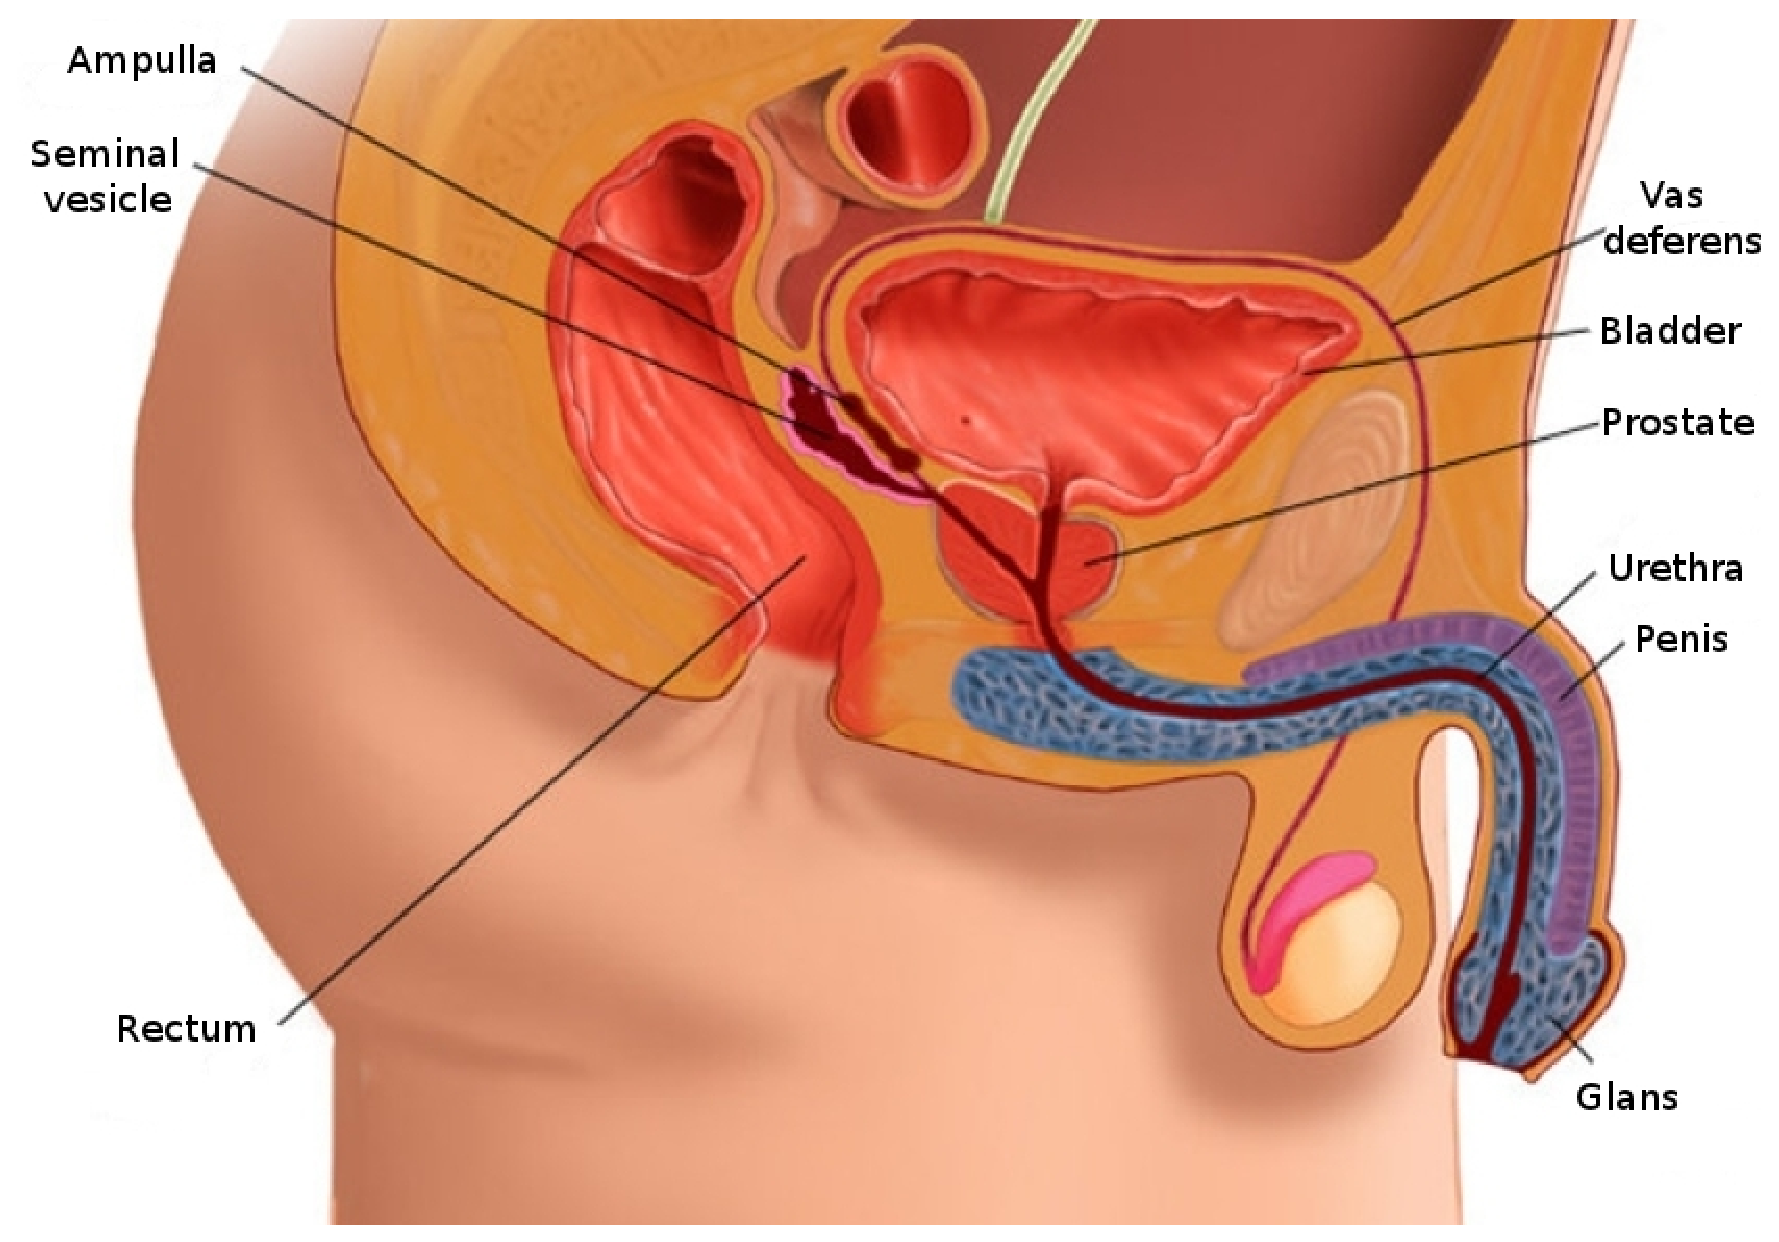
\includegraphics[height=0.25\textheight]{1_introduction/figures/anatomy/prostate2D.eps}
  \caption[Sagittal anatomy of prostate.]{Sagittal anatomy scheme of the male
    reproductive system (copyright by~\cite{Geckomedia2011}).}
  \label{fig:prostatelocation}
\end{figure}

\begin{figure}
  \centering
  \hspace*{\fill}
  \subfloat[Transverse anatomy of the prostate.]{
    \centering
    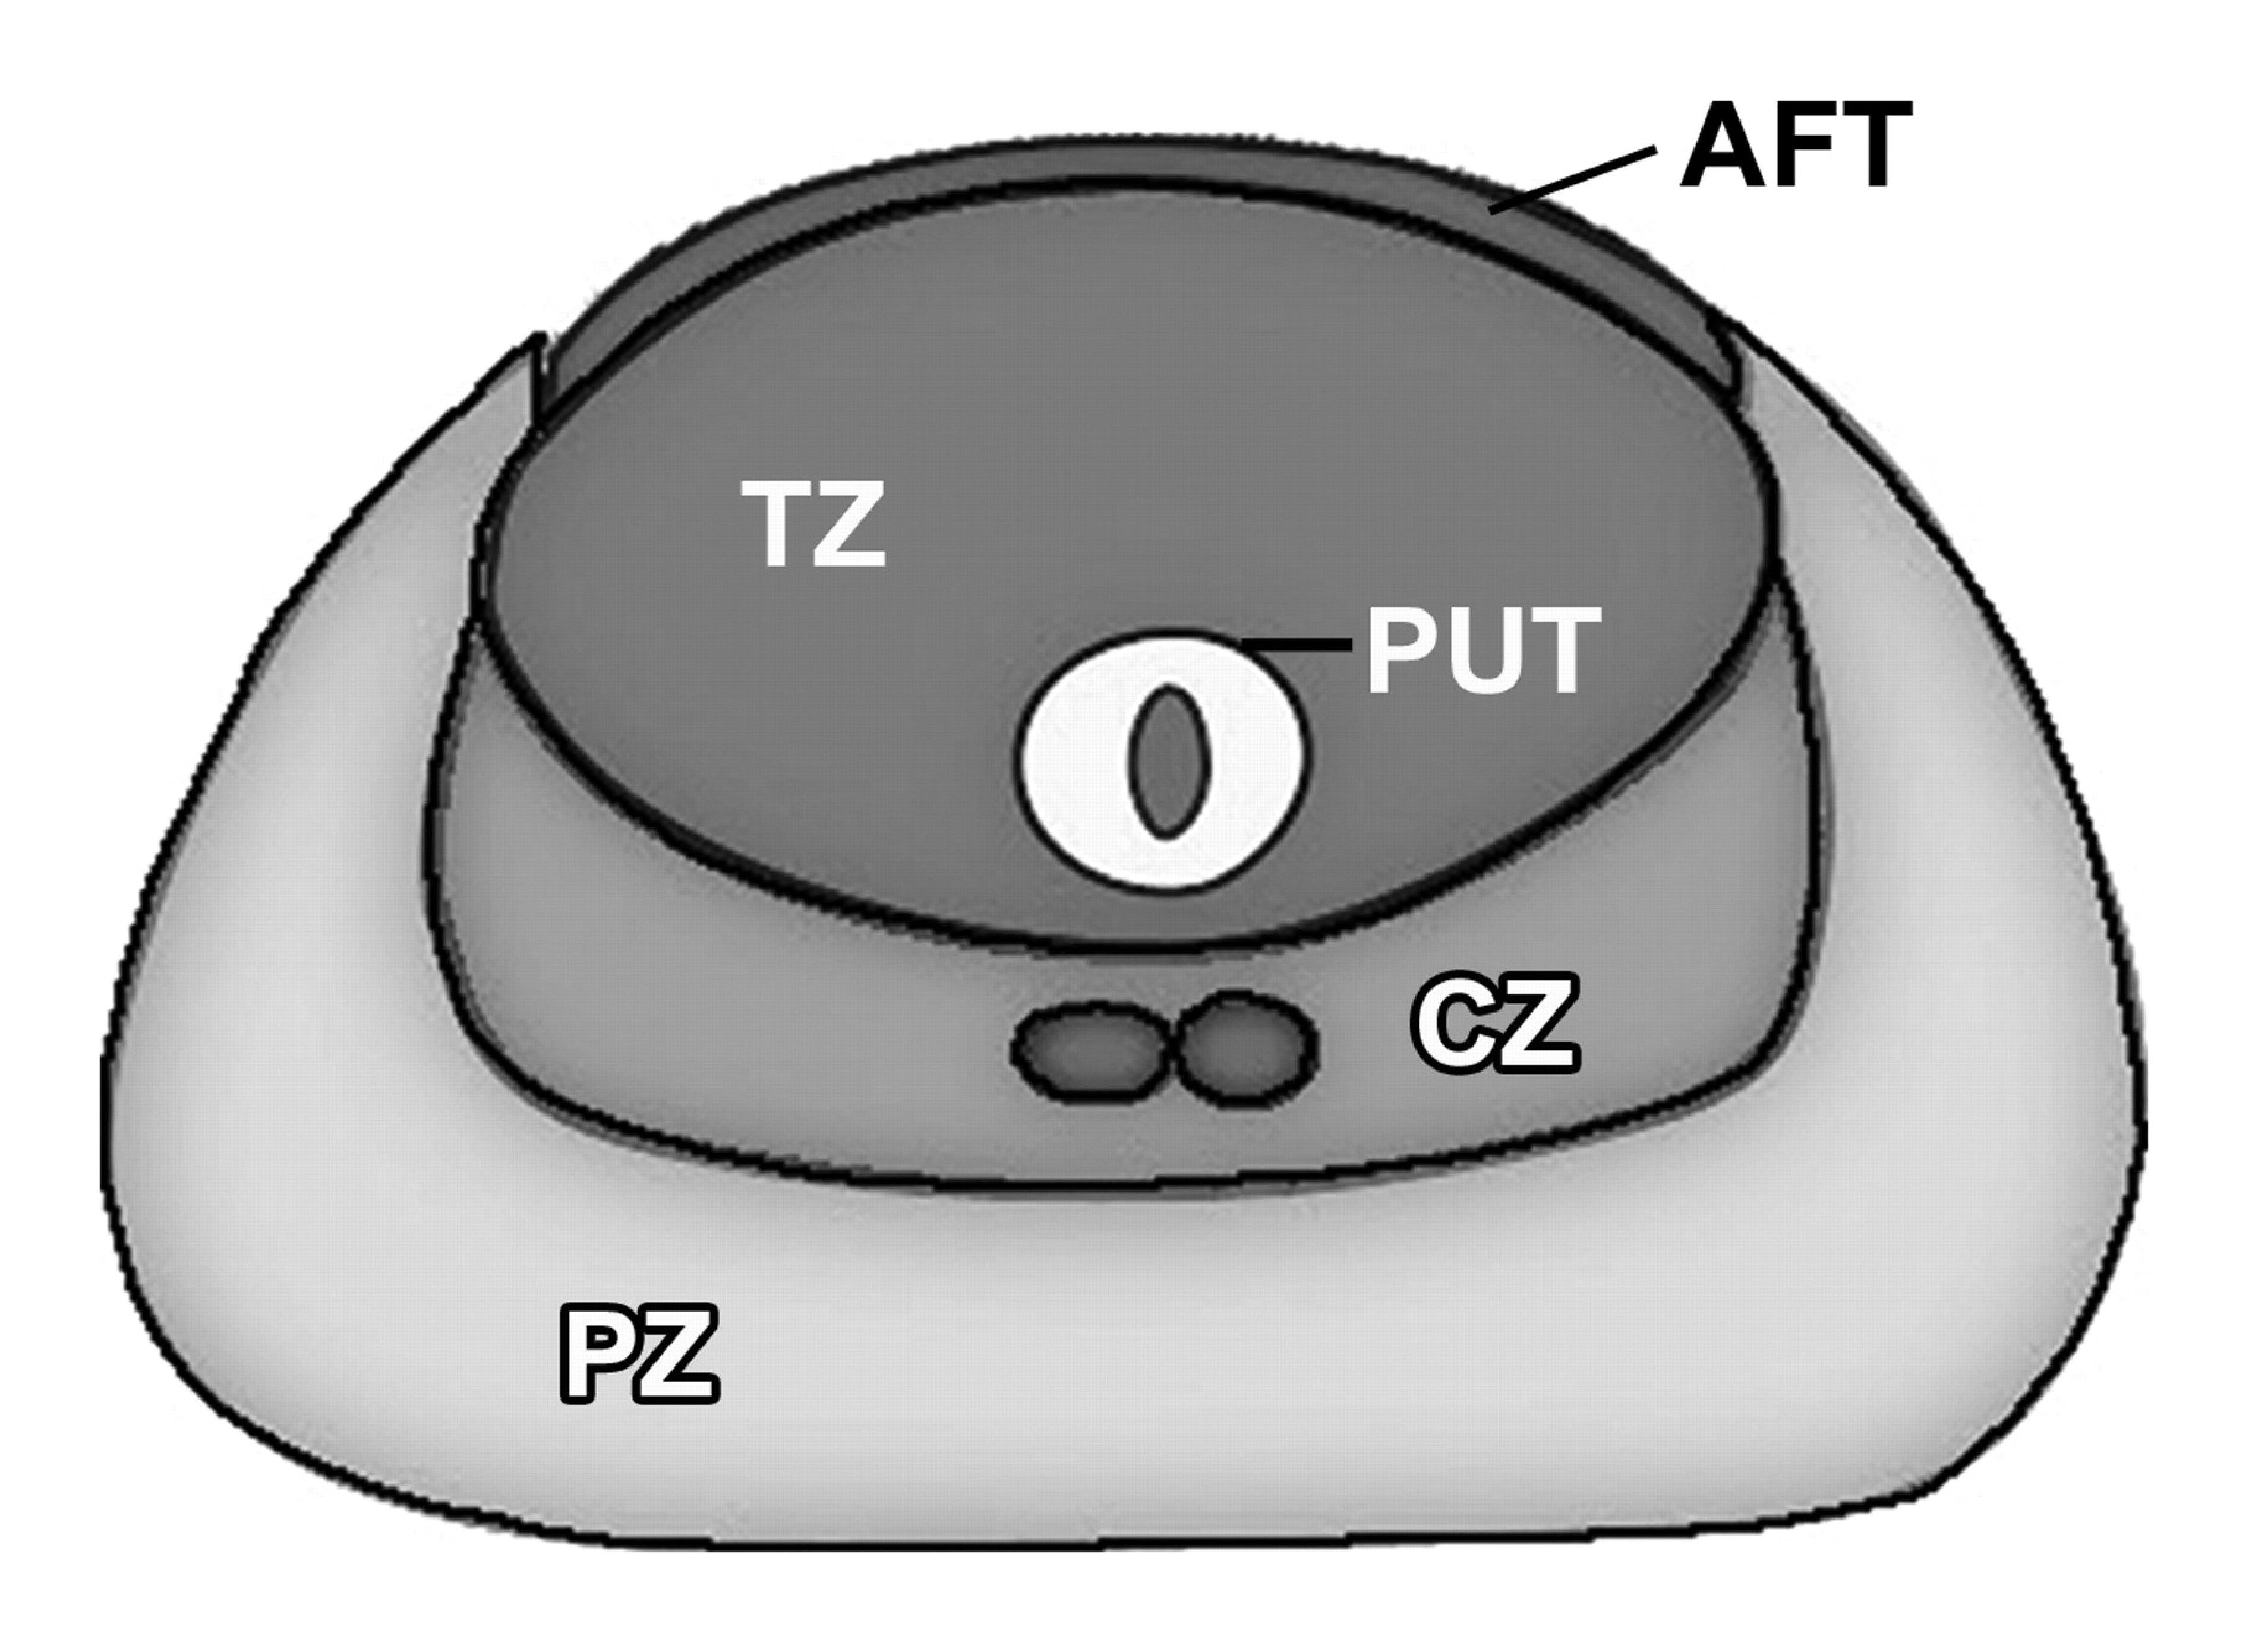
\includegraphics[height=0.15\textheight]{1_introduction/figures/anatomy/prostateTransverse.eps}
    \label{fig:anatomyProstateTransverse}}
  \hfill
  \subfloat[Sagittal anatomy of the prostate.]{
    \centering
    \includegraphics[height=0.23\textheight]{1_introduction/figures/anatomy/prostateSagital.eps}
    \label{fig:anatomyProstateSagittal}}\hspace*{\fill}
  \caption[Prostate anatomy.]{Prostate anatomy with division in different
    zones. \textit{AFT:} anterior fibromuscular tissue, \textit{CZ:} central
    zone, \textit{ED:} ejaculatory duct, \textit{NVB:} neurovascular bundle,
    \textit{PUT:} periurethral tissue, \textit{PZ:} peripheral zone,
    \textit{U:} urethra, \textit{TZ:} transitional zone, \textit{B:} base,
    \textit{M:} median, \textit{A:} apex (copyright by~\cite{Choi2007}).}
  \label{fig:anatomyProstateZone}
\end{figure}

Prostate cancer \ac{cap} has been reported on a worldwide scale to be the
second most frequently diagnosed cancer of men accounting for
\SI{13.6}{\percent}~\cite{Ferlay2010}.
Statistically, in 2008, the number of new diagnosed cases has been estimated to
be $899,000$ with no less than $258,100$ deaths~\cite{Ferlay2010}.
In United States, aside from skin cancer, \ac{cap} is declared to be the most
commonly diagnosed cancer among men, implying that approximately 1 in 6 men
will be diagnosed with \ac{cap} during their lifetime and 1 in 36 will die from
this disease, causing \ac{cap} to be the second most common cause of cancer
death among men~\cite{Siegel2013,Society2013}.

Despite active research to determine the causes of \ac{cap}, a fuzzy list of
risk factors has arisen~\cite{Society2010}.
The etiology has been linked to the following factors~\cite{Society2010}: (i)
family history~\cite{Giovannucci2007,Steinberg1990}, (ii) genetic
factors~\cite{Freedman2006,Amundadottir2006,Agalliu2009}, (iii)
race-ethnicity~\cite{Giovannucci2007,Hoffman2001}, (iv)
diet~\cite{Giovannucci2007,Ma2009,Alexander2010}, and (v)
obesity~\cite{Giovannucci2007,Rodriguez2007}.
This list of risk factors alone cannot be used to diagnose \ac{cap} and in this
way, screening enables early detection and treatment.

\ac{cap} growth is characterized by two main types of
evolution~\cite{Strum2005}: slow-growing tumours, accounting for up to
\SI{85}{\percent} of all \acp{cap}~\cite{Lu-Yao2009}, progress slowly and
usually stay confined to the prostate gland.
For such cases, treatment can be substituted with active surveillance.
In contrast, the second variant of \acp{cap} develops rapidly and metastasises
from prostate gland to other organs, primarily the bones~\cite{Oster2013}.
Bone metastases, being an incurable disease, significantly affects the
morbidity and mortality rate~\cite{Ye2007}.
Hence, the results of the surveillance have to be trustworthy to
distinguish aggressive from slow-growing \ac{cap}.

\ac{cap} is more likely to come into being in specific regions of the prostate.
In that respect, around \SIrange{70}{80}{\percent} of \acp{cap} originate in
\ac{pz} whereas \SIrange{10}{20}{\percent} in
\ac{tz}~\cite{Carrol1987,McNeal1988,Stamey1998}.
Only about \SI{5}{\percent} of \acp{cap} occur in
\ac{cz}~\cite{McNeal1988,Cohen2008}.
However, those cancers appear to be more aggressive and more likely to invade
other organs due to their locations~\cite{Cohen2008}.

\subsection{\acs*{cap} screening and imaging techniques}\label{sec:intro:screening}

Current \ac{cap} screening consists of three different stages.
First, \ac{psa} control is performed to distinguish between low- and high-risk
\ac{cap}.
To assert such diagnosis, samples are taken during prostate biopsy and finally
analyzed to evaluate the prognosis and the stage of \ac{cap}.
In this section, we present a detailed description of the current screening as
well as its drawbacks.

Since its introduction in mid-1980s, \ac{psa} is widely used for \ac{cap}
screening~\cite{Etzioni2002}.
A higher-than-normal level of \ac{psa} can indicate an abnormality of the
prostate either as a \ac{bph} or a cancer~\cite{Hoeks2011}.
However, other factors can lead to an increased \ac{psa} level such as prostate
infections, irritations, a recent ejaculation, or a recent rectal
examination~\cite{Parfait2010}.
\ac{psa} is found in the bloodstream in two different forms: free \ac{psa}
accounting for about \SI{10}{\percent} and linked to another protein for the
remaining \SI{90}{\percent}.
A level of \ac{psa} higher than \SI{10}{\nano\gram\per\milli\liter} is
considered to be at risk~\cite{Parfait2010}.
If the \ac{psa} level is ranging from
\SIrange{4}{10}{\nano\gram\per\milli\liter}, the patient is considered as
suspicious~\cite{Barentsz2012}.
In that case, the ratio of free \ac{psa} to total \ac{psa} is computed; if the
ratio is higher than \SI{15}{\percent}, the case is considered as
pathological~\cite{Parfait2010}.

\Iac{trus} biopsy is carried out for cases which are considered pathological.
At least 6 different samples are taken randomly from the right and left parts
of the 3 different prostate zones: apex, median, and base.
These samples are further evaluated using the Gleason grading
system~\cite{Gleason1977}.
The scoring scheme to characterize the biopsy sample is composed of 5 different
patterns which correspond to grades ranging from 1 to 5.
A higher grade is associated with a poorer prognosis~\cite{Epstein2005}.
Then, in the Gleason system, 2 scores are assigned corresponding to (i) the
grade of the most present tumour pattern, and (ii) the grade of the second most
present tumour pattern~\cite{Epstein2005}.
A higher \ac{gs} indicates a more aggressive tumour~\cite{Epstein2005}.
Also, it should be noted that biopsy is an invasive procedure which can result
in serious infection or urine retention~\cite{Hara2005,Chou2011}.

Although \ac{psa} screening has been shown to improve early detection of
\ac{cap}~\cite{Chou2011}, its lack of reliability motivates further
investigations using \ac{mri}-based \ac{cad}.
Two reliable studies --- carried out in the United States~\cite{Andriole2009}
and in Europe~\cite{Schroeder2012, Hugosson2010} --- have attempted to assess
the impact of early detection of \ac{cap}, with diverging
outcomes~\cite{Chou2011,Heidenreich2013}.
The study carried out in Europe\footnote{The \ac{ersspc} started in the 1990s
  in order to evaluate the effect of \ac{psa} screening on mortality rate.}
concluded that \ac{psa} screening reduces CaP-related mortality by
\SIrange{21}{44}{\percent}~\cite{Schroeder2012, Hugosson2010}, while the
American\footnote{The \ac{plco} cancer screening trial is carried out in the
  United States and intends to ascertain the effects of screening on mortality
  rate.} trial found no such effect~\cite{Andriole2009}.
However, both studies agree that \ac{psa} screening suffers from low
specificity, with an estimated rate of \SI{36}{\percent}~\cite{Schroder2008}.
Both studies also agree that over-treatment is an issue: decision making
regarding treatment is further complicated by difficulties in evaluating the
aggressiveness and progression of \ac{cap}~\cite{Delpierre2013}.

Hence, new screening methods should be developed with improved specificity of
detection as well as more accurate risk assessment (i.e., aggressiveness and
progression).
Current research is focused on identifying new biological markers to replace
\ac{psa}-based screening~\cite{Bourdoumis2010,Morgan2011,Brenner2013}.
Until such research comes to fruition, these needs can be met through
active-surveillance strategy using \ac{mpmri}
techniques~\cite{Hoeks2011,Moore2013}.
An \ac{mri}-\acs{cad} system, which is an area of active research and forms the
focus of this thesis, can be incorporated into this screening strategy allowing
a more systematic and rigorous follow-up.

Another weakness of the current screening strategy lies in the fact that
\ac{trus} biopsy does not provide trustworthy results.
Due to its ``blind'' nature, there is a chance of missing aggressive tumours or
detecting microfocal ``cancers'', which influences the
aggressiveness-assessment procedure~\cite{Noguchi2001}.
As a consequence, over-diagnosis is estimated at up to
\SI{30}{\percent}~\cite{Haas2007}, while missing clinically significant
\ac{cap} is estimated at up \SI{35}{\percent}~\cite{Taira2010}.
In an effort to solve both issues, alternative biopsy approaches have been
explored.
\ac{mri}/\ac{us}-guided biopsy has been shown to outperform standard \ac{trus}
biopsy~\cite{Delongchamps2013}.
There, \ac{mpmri} images are fused with \ac{us} images in order to improve
localization and aggressiveness assessment to carry out biopsies.
Human interaction plays a major role in biopsy sampling which can lead to low
repeatability; by reducing potential human errors at this stage, the \acs{cad}
framework can be used to improve repeatability of examination.
\ac{cap} detection and diagnosis can benefit from the use of \acs{cad} and
\ac{mri} techniques.

In an effort to improve the current stage of \ac{cap} diagnosis and detection,
this thesis is intended to develop the principles of a \ac{mpmri}-\acs{cad}
system.
A description of the different \ac{mri} modalities is presented in
\acs{chp}\,\ref{chap:2}.

\subsection{\acs*{cad} systems for \acs*{cap}}\label{sec:intro:cad}
During the last century, physicists have focused on constantly innovating in
terms of imaging techniques assisting radiologists to improve cancer detection
and diagnosis.
However, human diagnosis still suffers from low repeatability, synonymous with
erroneous detection or interpretations of abnormalities throughout clinical
decisions~\cite{Giger2008,Hambrock2013}.
These errors are driven by two majors causes~\cite{Giger2008}: observer
limitations (e.g., constrained human visual perception, fatigue or distraction)
and the complexity of the clinical cases themselves, for instance due to
imbalanced data --- the number of healthy cases is more abundant than malignant
cases --- or overlapping structures.

Computer vision has given rise to many promising solutions, but, instead of
focusing on fully automatic computerized systems, researchers have aimed at
providing computer image analysis techniques to aid radiologists in their
clinical decisions~\cite{Giger2008}.
In fact, these investigations brought about both concepts of \ac{cade} and
\ac{cadx} grouped under the acronym \ac{cad}.
Since those first steps, evidence has shown that \ac{cad} systems enhance the
diagnosis performance of radiologists.
\citeauthor{Chan1999} reported a significant \SI{4}{\percent} improvement in
breast cancer detection~\cite{Chan1999}, which has been confirmed in later
studies~\cite{Dean2006}.
Similar conclusions have been drawn in the case of lung nodule
detection~\cite{Li2004}, colon cancer~\cite{Petrick2008}, or \ac{cap} as
well~\cite{Hambrock2013}.
\citeauthor{Chan1999} also hypothesized that \acs{cad} systems will be even
more efficient assisting inexperienced radiologists than senior
radiologists~\cite{Chan1999}.
That hypothesis has been tested by \citeauthor{Hambrock2013} and confirmed in
case of \ac{cap} detection~\cite{Hambrock2013}.
In this particular study, inexperienced radiologists obtained equivalent
performance to senior radiologists, both using \acs{cad} whereas the accuracy
of their diagnosis was significantly poorer without \ac{cad}'s help.

In contradiction with the aforementioned statement, \ac{cad} for \ac{cap} is a
young technology due to the fact that is based on a still young imaging
technology: \ac{mri}~\cite{Hegde2013}.
Indeed, four distinct \ac{mri} modalities are employed in \ac{cap} diagnosis
which have been mainly developed after the mid-1990s: (i)
\ac{t2w}-\ac{mri}~\cite{Hricak1983}, (ii)
\ac{dce}-\ac{mri}~\cite{HuchBoni1995}, (iii) \ac{mrsi}~\cite{Kurhanewicz1996},
and (iv) \ac{dw}-\ac{mri}~\cite{Scheidler1999}.
In addition, the increase of magnetic field strength in clinical settings, from
\SIrange{1.5}{3}{\tesla}, and the development of endorectal coils, both
improved image spatial resolution~\cite{Swanson2001} needed to perform more
accurate diagnosis.
It is for this matter that the development of \ac{cad} for \ac{cap} is still
lagging behind the fields stated above.

The further sections aim at first, to provide an overview of the current
state-of-the-art of \ac{cad} for \ac{cap} and later, according to the drawn
conclusions, to propose a \ac{cad} which takes advantages of \ac{mpmri}
modalities.
A review of the current proposed \ac{cad} for \ac{cap} is presented in
\acs{chp}\,\ref{chap:3}.


\section{\acs*{mri} Techniques}\label{chap:2}
\graphicspath{{2_modality/figures/}}

% \section{MRI principles}\label{sec:chp2:principles}

\Ac{mri} provides promising imaging techniques to overcome the drawbacks of
current clinical screening techniques mentioned in \acs{sec}\,\ref{chap:1}.
Unlike \ac{trus} biopsy, \ac{mri} examination is a non-invasive protocol and
has been shown to be the most accurate and harmless technique currently
available~\cite{Turkbey2012}.
In this section, we review different \ac{mri} imaging techniques developed for
\ac{cap} detection and diagnosis.
Features strengthening each modality will receive particular attention together
with their drawbacks.
Commonly, these features form the basis for developing analytic tools and
automatic algorithms.
However, we refer the reader to
\acs{sec}\,\ref{subsec:chp3:img-clas:CADX-fea-dec} for more details on
automatic feature detection methods since they are part and parcel of the
\acs{cad} framework.

\begin{figure}
  \centering
  \hspace*{\fill}
  \subfloat[\acs*{t2w}-\acs*{mri} slice of a healthy prostate acquire with a
  \SI{1.5}{\tesla} \acs*{mri} with an endorectal coil. The blue contour
  represents the \acs*{cg} while the \acs*{pz} corresponds to the green
  contour.]{\label{subfig:t2whealthy}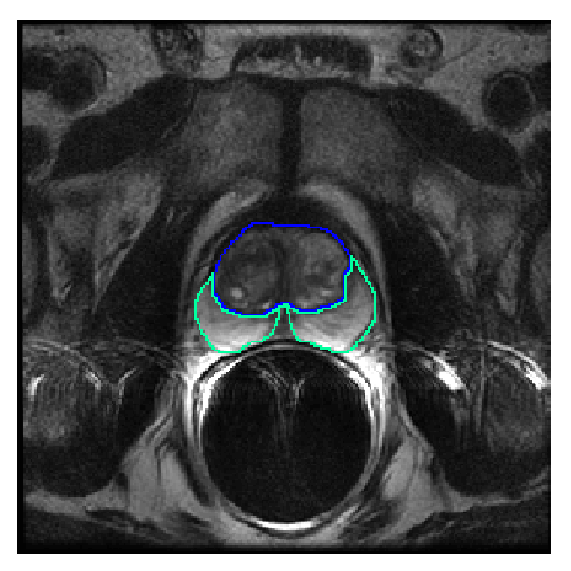
\includegraphics[width=0.3\linewidth]{2_modality/figures/t2w/t2w_healthy.eps}}
  \hfill
  \subfloat[\acs*{t2w}-\acs*{mri} slice of a prostate with a \acs*{cap}
  highlighted in the \acs*{pz} using a \SI{3}{\tesla} \acs*{mri} scanner
  without an endorectal
  coil.]{\label{subfig:t2wcancerpz}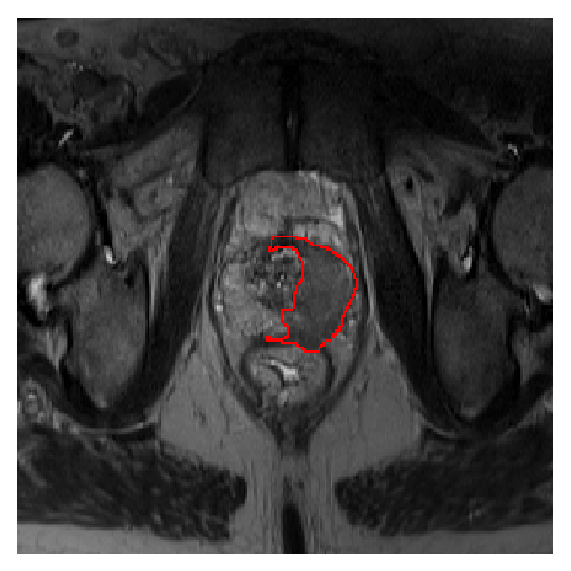
\includegraphics[width=0.3\linewidth]{2_modality/figures/t2w/t2w_cancer_pz.eps}}
  \hfill
  \subfloat[\acs*{t2w}-\acs*{mri} slice of a prostate with a \acs*{cap}
  highlighted in the \acs*{cg} using a \SI{1.5}{\tesla} \acs*{mri} scanner with
  an endorectal
  coil.]{\label{subfig:t2wcancercg}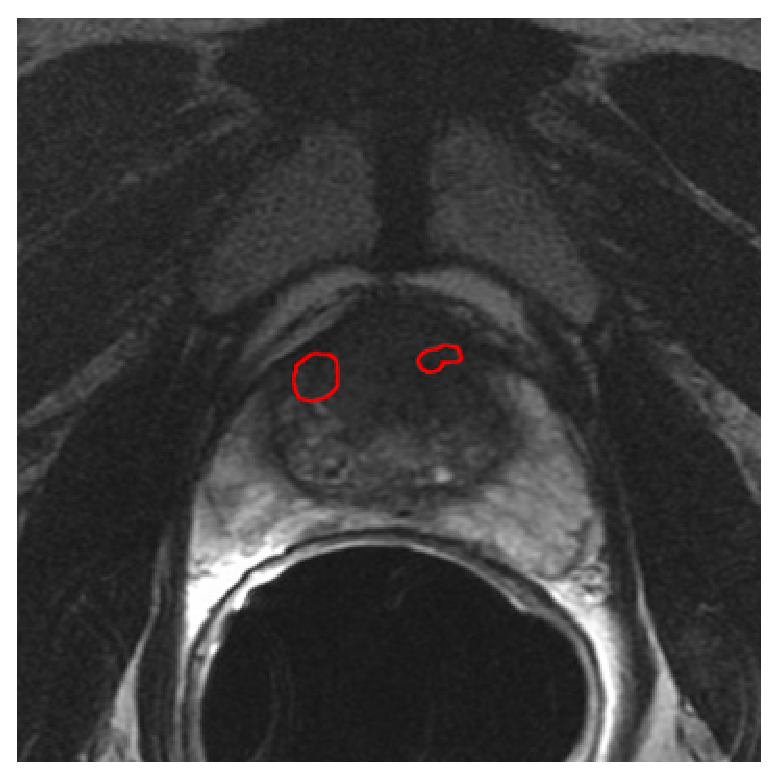
\includegraphics[width=0.3\linewidth]{2_modality/figures/t2w/t2w_cancer_cg.eps}}
  \hspace*{\fill}
  \caption[Rendering of \acs*{t2w}-\acs*{mri} prostate images.]{Rendering of
    \acs*{t2w}-\acs*{mri} prostate image with both \SI{1.5}{\tesla} and
    \SI{3}{\tesla} \acs*{mri} scanner.}
  \label{fig:t2w}
\end{figure}

\subsection{\acs*{t2w}-\acs*{mri}}\label{subsec:chp2:imaging:t2w}
\ac{t2w}-\ac{mri} has been the first \ac{mri}-modality used to perform \ac{cap}
diagnosis using \ac{mri}~\cite{Hricak1983}.
Nowadays, radiologists make use of it for \ac{cap} detection, localization, and
staging purposes.
This imaging technique is well suited to render zonal anatomy of the
prostate~\cite{Barentsz2012}.

This modality relies on a sequence based on setting a long \ac{tr}, reducing
the T$_{1}$ effect in \ac{nmr} signal measured, and fixing the \ac{te} to
sufficiently large values in order to enhance the T$_{2}$ effect of tissues.
Thus, \ac{pz} and \ac{cg} tissues are well perceptible in these images.
The former is characterized by an intermediate/high-\ac{si} while the latter is
depicted by a low-\ac{si}~\cite{Hricak1987}.
An example of a healthy prostate is shown in \acs{fig}\,\ref{subfig:t2whealthy}.

In \ac{pz}, round or ill-defined low-SI masses are synonymous with
\acp{cap}~\cite{Hricak1983} as shown in \acs{fig}\,\ref{subfig:t2wcancerpz}.
Detecting \ac{cap} in \ac{cg} is more challenging.
In fact both normal \ac{cg} tissue and malignant tissue, have a low-\ac{si} in
\ac{t2w}-\ac{mri}, reinforcing difficulties to distinguish one among them.
However, \acp{cap} in \ac{cg} appear often as homogeneous mass possessing
ill-defined edges with lenticular or ``water-drop''
shapes~\cite{Akin2006,Barentsz2012} as depicted in
\acs{fig}\,\ref{subfig:t2wcancercg}.

\ac{cap} aggressiveness has been shown to be inversely correlated with \ac{si}.
Indeed, \acp{cap} assessed with a \ac{gs} of 4-5 implied lower \ac{si} than the
one with a \ac{gs} of 2-3~\cite{Wang2008}.

In spite of the availability of these useful and encouraging features, the
\ac{t2w} modality lacks reliability~\cite{Kirkham2006,Hoeks2011}.
Sensitivity is affected by the difficulties in detecting cancers in
\ac{cg}~\cite{Kirkham2006} while specificity rate is highly affected by
outliers~\cite{Barentsz2012}.
In fact, various conditions emulate patterns of \ac{cap} such as \ac{bph},
post-biopsy hemorrhage, atrophy, scars, and
post-treatment~\cite{Hricak1987,Quint1991,Scheidler1999,Cruz2002,Barentsz2012}.
These issues are partly addressed using more innovative and advanced modalities.

% T2 Map
\subsection{T$_2$ map} \label{subsec:chp2:imaging:t2}
As previously mentioned, \ac{t2w}-\ac{mri} modality shows low sensitivity.
Moreover, \ac{t2w}-\ac{mri} images are a composite of multiple
effects~\cite{Hegde2013}.
However, T$_2$ values alone have been shown to be more
discriminative~\cite{Liu2011} and highly correlated with citrate concentration,
a biological marker in \ac{cap}~\cite{Liney1996,Liney1997}.

T$_2$ values are computed using the characteristics of transverse relaxation
which is formalized as in \acs{eq}\,\eqref{eq:tramag}.

\begin{equation}
  M_{xy}(t) = M_{xy}(0) \exp \left( - \frac{t}{\text{T}_2} \right) \ ,
  \label{eq:tramag}
\end{equation}

\noindent where $M_{xy}(0)$ is the initial value of $M_{xy}(t)$ and T$_2$ is
the relaxation time.

By rearranging \acs{eq}\,\eqref{eq:tramag}, T$_2$ map is computed by performing
a linear fitting on the model presented in \acs{eq}\,\eqref{eq:t2map} using
several TE, $t=\{ \text{TE}_1,\text{TE}_2, \dotsc ,\text{TE}_m \}$.

\begin{equation}
  \ln \left[ \frac{M_{xy}(t)}{M_{xy}(0)} \right] = - \frac{t}{\text{T}_2} \ .
  \label{eq:t2map}
\end{equation}

The \Ac{fse} sequence has been shown to be particularly well suited in order to
build a T$_2$ map and obtain accurate T$_2$ values~\cite{Liney1996a}.
Similar to \ac{t2w}-\ac{mri}, T$_2$ values associated with \ac{cap} are
significantly lower than those of healthy tissues~\cite{Liney1996,Gibbs2001}.

\begin{figure}
  \centering
  \hspace*{\fill}
  \subfloat[\acs*{t1w}-\acs*{mri} image where the cancer is delimited by the
  red contour. The green area was still not invaded by the
  \acs*{cap}]{\label{subfig:t1w}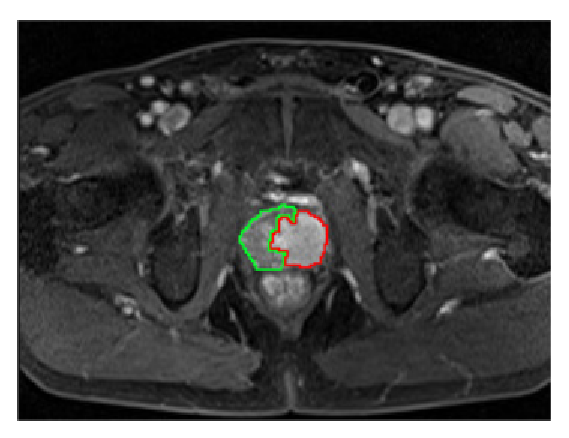
\includegraphics[width=0.4\linewidth]{2_modality/figures/dce/slice.eps}}
  \hfill
  \subfloat[Enhancement curve computed during the \acs*{dce}-\acs*{mri}
  analysis. The red curve is typical from \acs*{cap} cancer while the green
  curve is characteristic of healthy
  tissue.]{\label{subfig:dce}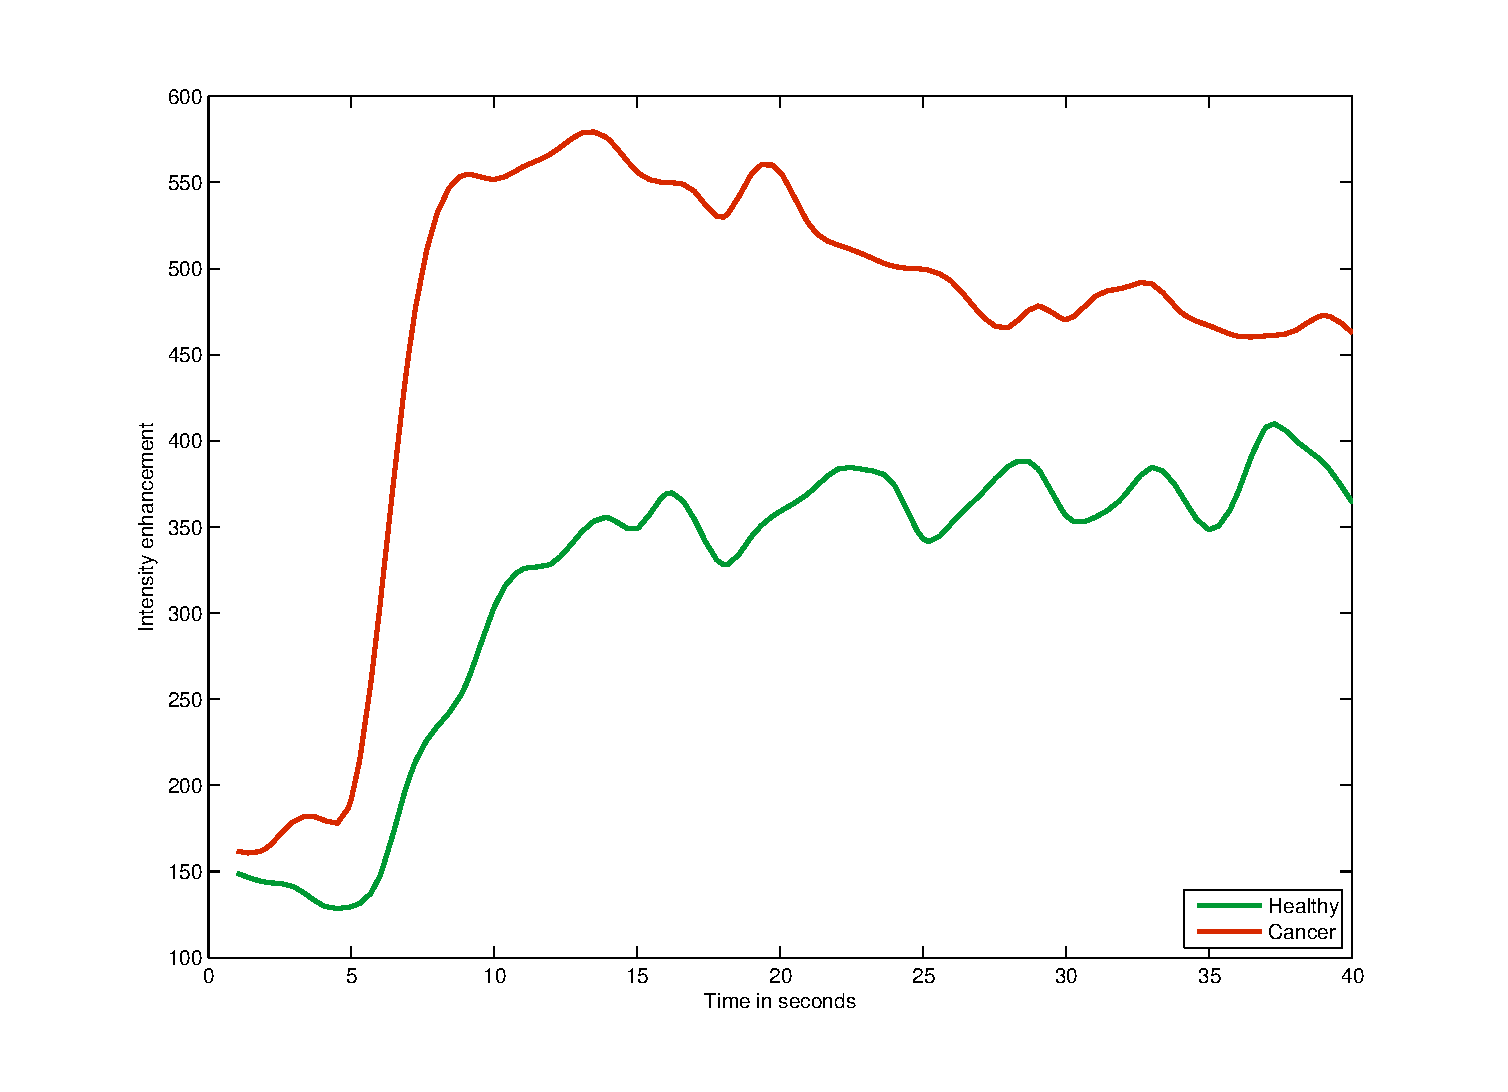
\includegraphics[width=0.45\linewidth]{2_modality/figures/dce/dce_cancer_healthy.eps}}
  \hspace*{\fill}
  \caption[Enhancement of \acs*{dce}-\acs*{mri} signal.]{Illustration of
    typical enhancement signal observed in \acs*{dce}-\acs*{mri} analysis
    collected with a \SI{3}{\tesla} \acs*{mri} scanner.}
  \label{fig:dceana}
\end{figure}

\subsection{\acs*{dce}-\acs*{mri}}\label{subsec:chp2:imaging:dce}
\Ac{dce}-\ac{mri} is an imaging technique which exploits the vascularity
characteristic of tissues.
Contrast media, usually gadolinium-based, is injected intravenously into the
patient.
The media extravasates from vessels to \ac{ees} and is released back into the
vasculature before being eliminated by the kidneys~\cite{Gribbestad2005}.
Furthermore, the diffusion speed of the contrast agent may vary due to several
parameters: (i) the permeability of the micro-vessels, (ii) their surface area,
and (iii) the blood flow~\cite{Padhani2002}.

Healthy \ac{pz} is mainly made up of glandular tissue, around
\SI{70}{\percent}~\cite{Choi2007}, which implies a reduced interstitial space
restricting exchanges between vessels and
\ac{ees}~\cite{Buckley2004,Niekerk2009}.
Normal \ac{cg} has a more disorganized structure, composed of mainly fibrous
tissue~\cite{Choi2007,Hoeks2011}, which facilitates the arrival of the contrast
agent in \ac{ees}~\cite{Niekerk2013}.
To understand the difference between contrast media kinetic in malignant
tumours and the two previous behaviours mentioned, one has to focus on the
process known as angiogenesis~\cite{Carmeliet2000}.
In order to ensure growth, malignant tumours produce and release angiogenic
promoter substances~\cite{Carmeliet2000}.
These molecules stimulate the creation of new vessels towards the
tumour~\cite{Carmeliet2000}.
However, the new vessel networks in tumours differ from those present in
healthy tissue~\cite{Gribbestad2005}.
They are more porous due to the fact that their capillary walls have a large
number of ``openings''~\cite{Gribbestad2005,Choi2007}.
In contrast to healthy cases, this increased vascular permeability results in
increased contrast agent exchanges between vessels and
\ac{ees}~\cite{Verma2012}.

By making use of the previous aspects, \ac{dce}-\ac{mri} is based on an
acquisition of a set of \ac{t1w}-\ac{mri} images over time.
The gadolinium-based contrast agent shortens T$_1$ relaxation time enhancing
contrast in \ac{t1w}-\ac{mri} images.
The aim is to post-analyze the pharmacokinetic behaviour of the contrast media
concentration in prostate tissues~\cite{Verma2012}.
The image analysis is carried out in two dimensions: (i) in the spatial domain
on a pixel-by-pixel basis and (ii) in the time domain corresponding to the
consecutive images acquired with the \ac{mri}.
Thus, for each spatial location, a signal linked to contrast media
concentration is measured as shown in
\acs{fig}\,\ref{subfig:dce}~\cite{Tofts2010}.

By taking the above remarks into account, \acp{cap} is characterized by a
signal having an earlier and faster enhancement and an earlier wash-out ---
i.e, the rate of the contrast agent flowing out of the tissue --- as shown in
\acs{fig}\,\ref{subfig:dce}~\cite{Verma2012}.
Three different approaches exist to analyze these signals with the aim of
labelling them as corresponding to either normal or malignant tissues.

Qualitative analysis is based on a qualitative assessment of the signal
shape~\cite{Hoeks2011}.
Quantitative approaches consist of inferring pharmocokinetic parameter
values~\cite{Tofts2010}.
Those parameters are part of mathematical-pharmacokinetic models which are
directly based on physiological exchanges between vessels and \ac{ees}.
Several pharmacokinetic models have been proposed such as the Kety
model~\cite{Kety1951}, the Tofts model~\cite{Tofts1997}, and mixed
models~\cite{Larsson1996,StLawrence1998}.
The last family of methods mixed both approaches and are grouped together under
the heading of semi-quantitative methods.
They rely on shape characterization using mathematical modelling to extract a
set of parameters such as wash-in gradient, wash-out, integral under the curve,
maximum signal intensity, time-to-peak enhancement, and start of
enhancement~\cite{Hoeks2011,Verma2012}.
These parameters are depicted in \acs{fig}\,\ref{fig:dceparam}.
It has been shown that semi-quantitative and quantitative methods improve
localization of \ac{cap} when compared with qualitative
methods~\cite{Rosenkrantz2013}.
\Ac{sec}~\ref{subsubsec:chp3:img-clas:CADX-fea-dec:DCE-fea} provides a full
description of quantitative and semi-quantitative approaches.

\ac{dce}-\ac{mri} combined with \ac{t2w}-\ac{mri} has shown to enhance
sensitivity compared to \ac{t2w}-\ac{mri}
alone~\cite{Jager1997,Kim2005,Schlemmer2004,Zelhof2009}.
Despite this fact, \ac{dce}-\ac{mri} possesses some drawbacks.
Due to its ``dynamic'' nature, patient motions during the image acquisition
lead to spatial mis-registration of the image set~\cite{Verma2012}.
Furthermore, it has been suggested that malignant tumours are difficult to
distinguish from prostatitis located in \ac{pz} and \ac{bph} located in
\ac{cg}~\cite{Hoeks2011,Verma2012}.
These pairs of tissues tend to have similar appearances.
Later studies have shown that \acp{cap} in \ac{cg} do not always manifest in
homogeneous fashion.
Indeed, tumours in this zone can present both hypo-vascularization and
hyper-vascularization which illustrates the challenge of \ac{cap} detection in
\ac{cg}~\cite{Niekerk2013}.

\begin{figure}
  \centering
  \hspace*{\fill}
  \subfloat[\acs*{dw}-\acs*{mri} image acquired with a \SI{1.5}{\tesla}
  \acs*{mri} scanner. The cancer corresponds to the high \acs*{si} region
  highlighted in
  red.]{\label{subfig:dwi}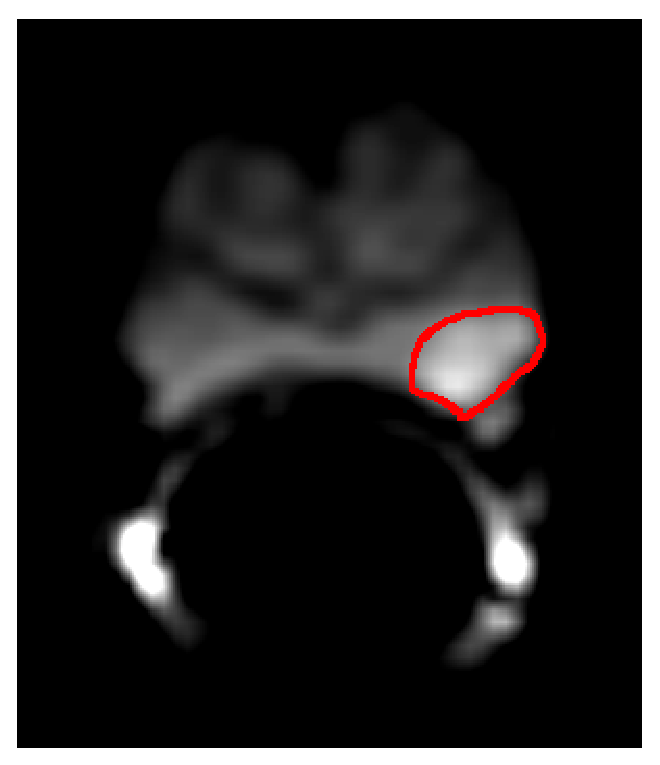
\includegraphics[width=0.25\linewidth]{2_modality/figures/dwi/dwi_cancer.eps}}
  \hfill
  \subfloat[\acs*{adc} map computer after acquisition of \acs*{dw}-\acs*{mri}
  images with \SI{1.5}{\tesla} \acs*{mri} scanner. The cancer corresponds to
  the low \acs*{si} region highlighted in
  red.]{\label{subfig:adc}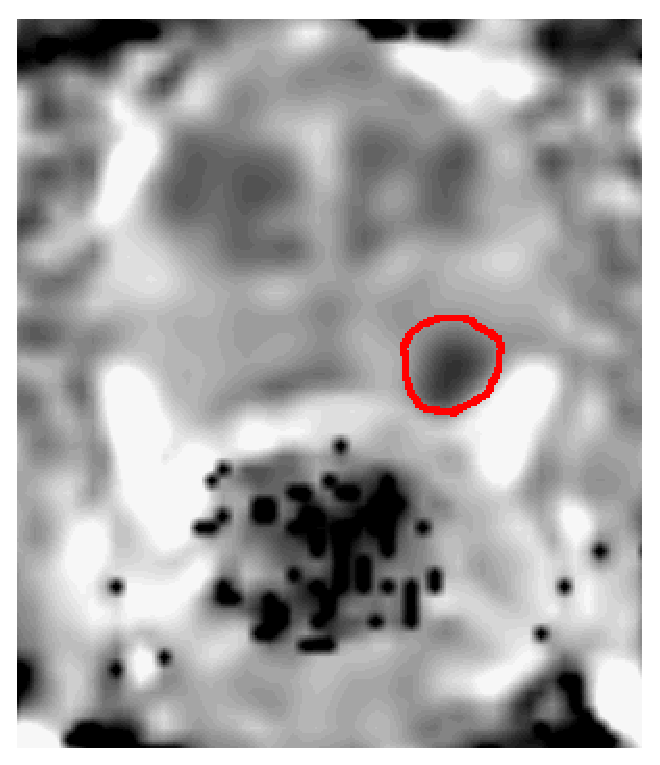
\includegraphics[width=0.25\linewidth]{2_modality/figures/dwi/adc_cancer.eps}}
  \hspace*{\fill}
  \caption[Example of \acs*{dw}-\acs*{mri} and \acs*{dce} map.]{Illustration of
    of \acs*{dw}-\acs*{mri} and \acs*{adc} map. The signal intensity
    corresponding to cancer are inversely correlated on these modalities.}
  \label{fig:dwi}
\end{figure}

\subsection{\acs*{dw}-\acs*{mri}}\label{subsec:chp2:imaging:dw}
As previously mentioned in the introduction, \ac{dw}-\ac{mri} is the most
recent \ac{mri} imaging technique aiming at \ac{cap} detection and
diagnosis~\cite{Scheidler1999}.
This modality exploits the variations in the motion of water molecules in
different tissues~\cite{LeBihan1988,Koh2007}.

The distinction between healthy and \ac{cap} in \ac{dw}-\ac{mri} is based on
the following physiological bases.
On the one hand, \ac{pz}, as previously mentioned, is mainly a glandular and
tubular structure allowing water molecules to move
freely~\cite{Choi2007,Hoeks2011}.
On the other hand, \ac{cg} is made up of muscular or fibrous tissue causing the
motion of the water molecules to be more constrained and heterogeneous than in
\ac{pz}~\cite{Hoeks2011}.
Then, \ac{cap} growth leads to the destruction of normal glandular structure
and is associated with an increase in cellular
density~\cite{Hoeks2011,Koh2007,Somford2008}.
Furthermore, these factors both have been shown to be inversely correlated with
water diffusion~\cite{Koh2007,Somford2008}: higher cellular density implies a
restricted water diffusion.
Thus, water diffusion in \ac{cap} will be more restricted than both healthy
\ac{pz} and \ac{cg}~\cite{Koh2007,Hoeks2011}.

From the \ac{nmr} principle side, \ac{dw}-\ac{mri} sequence produces contrasted
images due to variation of water molecules motion.
The method is based on the fact that the signal in \ac{dw}-\ac{mri} images is
inversely correlated to the degree of random motion of water
molecules~\cite{Huisman2003}.
In fact, gradients are used in \ac{dw}~\ac{mri} modality to encode spatial
location of nuclei temporarily.
Simplifying the problem in only one direction, a gradient is applied in that
direction, dephasing the spins of water nuclei.
Hence, the spin phases vary along the gradient direction depending of the
gradient intensity at those locations.
Then, a second gradient is applied aiming at cancelling the spin dephasing.
Thus, the immobile water molecules will be subject to the same gradient
intensity as the initial one while moving water molecules will be subject to a
different gradient intensity.
Thus, spins of moving water molecules will stay dephased whereas spins of
immobile water molecules will come back in phase.
As a consequence, a higher degree of random motion results in a more
significant signal loss whereas a lower degree of random motion is synonymous
with lower signal loss~\cite{Huisman2003}.
Under these conditions, the \ac{mri} signal is measured as:

\begin{align}
  M_{x,y}\left(t,b\right) & = M_{x,y}(0) \exp \left( - \frac{t}{\text{T}_2} \right) S_{\text{ADC}}(b) \ , \label{eq:t2dif} \\
  S_{\text{ADC}}(b) & = \exp \left( -b \times \text{ADC} \right) \ , \label{eq:dif}
\end{align}

\noindent where $S_{\text{ADC}}$ refers to signal drop due to diffusion effect,
$\text{ADC}$ is the \acl{adc}, and $b$ is the attenuation coefficient depending
only on the gradient pulses parameters: (i) gradient intensity and (ii)
gradient duration~\cite{LeBihan1986}.

By using this formulation, image acquisition with a parameter $b$ equal to
\SI{0}{\second\per\milli\metre\squared} corresponds to a \ac{t2w}-\ac{mri}
acquisition.
Then, increasing the attenuation coefficient $b$ --- i.e., increase gradient
intensity and duration --- enhances the contrast in \ac{dw}-\ac{mri} images.

To summarize, in \ac{dw}-\ac{mri} images, \acp{cap} are characterized by
high-\ac{si} compared to normal tissues in \ac{pz} and \ac{cg} as shown in
\acs{fig}\,\ref{subfig:dwi}~\cite{Barentsz2012}.
However, some tissues in \ac{cg} can look similar to \ac{cap} with higher
\ac{si}~\cite{Barentsz2012}.

Diagnosis using \ac{dw}-\ac{mri} combined with \ac{t2w}-\ac{mri} has shown a
significant improvement compared with \ac{t2w}-\ac{mri} alone and provides
highly contrasted images~\cite{Shimofusa2005,Padhani2011,Choi2007}.
As drawbacks, this modality suffers from poor spatial resolution and
specificity due to false positive detection~\cite{Choi2007}.
With a view to eliminate these drawbacks, radiologists use quantitative maps
extracted from \ac{dw}-\ac{mri}, which is presented in the next section.

\subsection{\acs*{adc} map}\label{subsec:chp2:imaging:adc}
The \ac{nmr} signal measured for \ac{dw}-\ac{mri} images is not only affected
by diffusion as shown in \acs{eq}\,\eqref{eq:t2dif}.
However, the signal drop --- \acs{eq}\,\eqref{eq:dif} --- is formulated such
that the only variable is the acquisition parameter $b$~\cite{LeBihan1986}.
The \ac{adc} is considered as a ``pure'' diffusion coefficient and is extracted
to build a quantitative map known as the \acs{adc} map.
From \acs{eq}\,\eqref{eq:t2dif}, it is clear that performing multiple
acquisitions only varying $b$ will not have any effect on the term  $M_{x,y}(0)
\exp \left( - \frac{t}{\text{T}_2} \right)$.
Thus, \acs{eq}\,\eqref{eq:t2dif} can be rewritten as:

\begin{equation}
  S(b) = S_0 \exp \left( -b \times \text{ADC} \right) \ .
  \label{eq:t2adcrew}
\end{equation}

To compute the \ac{adc} map, a minimum of two acquisitions are necessary: (i)
for $b$ equal to \SI{0}{\second\per\milli\metre\squared} where the measured
signal is equal to $S_0$, and (ii) $b_1$ greater than
\SI{0}{\second\per\milli\metre\squared}, typically
\SI{1000}{\second\per\milli\metre\squared}.
Then, the \ac{adc} map can be computed as:

\begin{equation}
  \text{ADC} = - \frac{\ln \left( \cfrac{S(b_1)}{S_0} \right) }{b_1} \ .
  \label{eq:adcres1}
\end{equation}

More accurate \ac{adc} maps are computed by acquiring a set of images with
different values for the parameter $b$ and fitting linearly a semi-logarithm
function using the model presented in \acs{eq}\,\eqref{eq:t2adcrew}.

Regarding the appearance of the \ac{adc} maps, it has been previously stated
that by increasing the value of $b$, the signal of \ac{cap} tissue increases
significantly.
Considering \acs{eq}\,\eqref{eq:adcres1}, the tissue appearance in the \ac{adc}
map is the inverse of \ac{dw}-\ac{mri} images.
Then, \ac{cap} tissue is associated with low-\ac{si} whereas healthy tissue
appears brighter as depicted in
\acs{fig}\,\ref{subfig:adc}~\cite{Barentsz2012}.

Similar to the gain achieved by \ac{dw}-\ac{mri}, diagnosis using \ac{adc} map
combined with \ac{t2w}-\ac{mri} significantly outperforms \ac{t2w}-\ac{mri}
alone~\cite{Doo2012,Choi2007}.
Moreover, it has been shown that \ac{adc} coefficient is correlated with
\ac{gs}~\cite{Hambrock2011,Itou2011,Peng2013}.

However, some tissues of the \ac{cg} mimic \ac{cap} with
low-\ac{si}~\cite{Kirkham2006} and image distortion can arise due to
hemorrhage~\cite{Choi2007}.
It has also been noted that a high variability of the \ac{adc} occurs between
different patients making it difficult to define a static threshold to
distinguish \ac{cap} from non-malignant tumours~\cite{Choi2007}.

\begin{figure}
  \centering
  \hspace*{\fill}
  \subfloat[Illustration of an \acs*{mrsi} spectrum of a healthy voxel acquired
  with a \SI{3}{\tesla}
  \acs*{mri}.]{\label{subfig:mrsihea}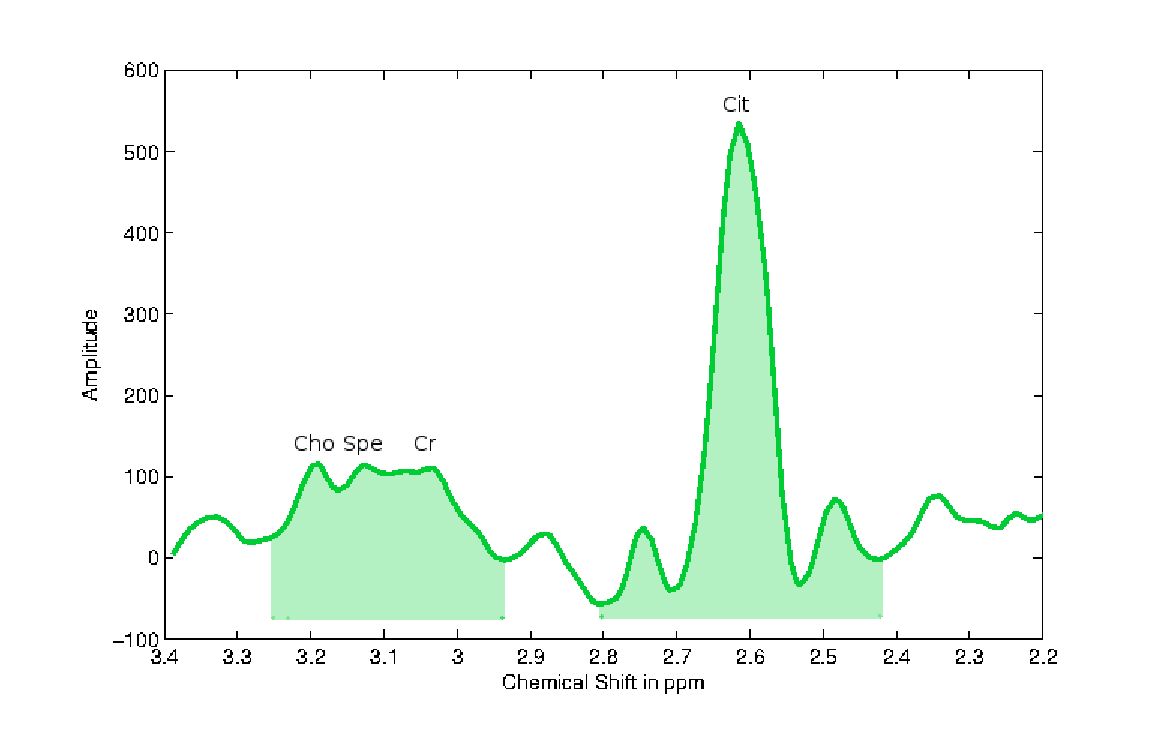
\includegraphics[width=0.45\linewidth]{2_modality/figures/mrsi/mrsi_healthy.eps}}
  \hfill
  \subfloat[Illustration of an \acs*{mrsi} spectrum of a cancerous voxel
  acquired with a \SI{3}{\tesla}
  \acs*{mri}.]{\label{subfig:mrsican}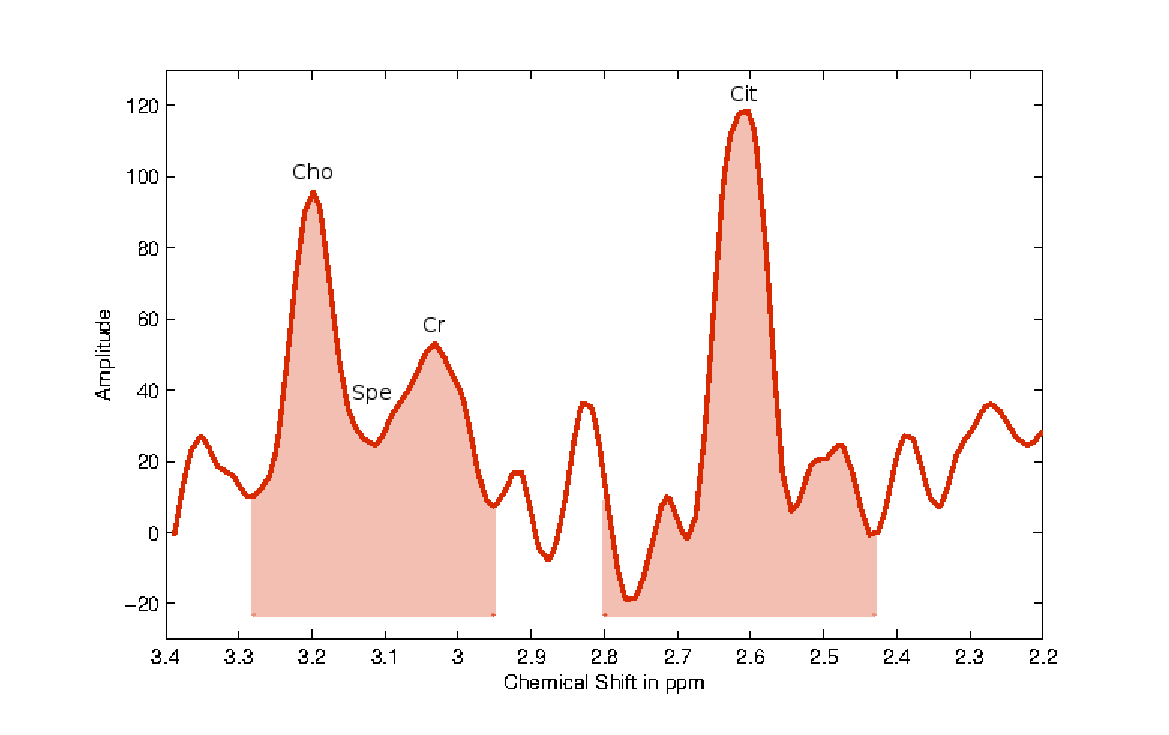
\includegraphics[width=0.45\linewidth]{2_modality/figures/mrsi/mrsi_cancer.eps}}
  \hspace*{\fill}
  \caption[Illustration of healthy and cancerous \acs*{mrsi}
  spectrum.]{Illustration of an \acs*{mrsi} spectrum for both healthy and
    cancerous voxels with a \SI{3}{\tesla} \acs*{mri}. The highlighted areas
    correspond to the related concentration of the metabolites which is
    computed by integrating the area under each peak. Acronyms: choline (Cho),
    spermine (Spe), creatine (Cr) and citrate (Cit).}
  \label{fig:mrsi}
\end{figure}

\subsection{\acs*{mrsi}}\label{subsec:chp2:imaging:mrsi}
\ac{cap} induces metabolic changes in the prostate compared with healthy tissue.
Thus, \ac{cap} detection can be carried out by tracking changes of metabolite
concentration in prostate tissue.
\ac{mrsi} is an \ac{nmr}-based technique which generates spectra of relative
metabolite concentration in \iac{roi}.

In order to track changes of metabolite concentration, it is important to know
which metabolites are associated with \ac{cap}.
To address this question, clinical studies identified three biological markers:
(i) citrate, (ii) choline, and (iii) polyamines composed mainly of spermine,
and in less abundance of spermidine and
putrescine~\cite{Awwad2012,Costello2006,Giskeodegard2013}.

Citrate is involved in the production and secretion of the prostatic fluid, and
the glandular prostate cells are associated with a high production of citrate
enabled by zinc accumulation by these same cells~\cite{Costello2006}.
However, the metabolism allowing the accumulation of citrate requires a large
amount of energy~\cite{Costello2006}.
In contrast, malignant cells do not have high zinc levels leading to lower
citrate levels due to citrate oxidization~\cite{Costello2006}.
Furthermore, this change results in a more energy-efficient metabolism enabling
malignant cells to grow and spread~\cite{Costello2006}.

An increased concentration of choline is related to \ac{cap}~\cite{Awwad2012}.
Malignant cell development requires epigenetic mechanisms resulting in
metabolic changes and relies on two mechanisms: \ac{dna} methylation and
phospholid metabolism which both result in choline uptake, explaining its
increased level in \ac{cap} tissue~\cite{Awwad2012}.
Spermine is also considered as a biological marker in
\ac{cap}~\cite{Graaf2000,Giskeodegard2013}.
In \ac{cap}, reduction of the ductal volume due to shifts in polyamine
homeostasis might lead to a reduced spermine concentration~\cite{Graaf2000}.

To determine the concentration of these biological markers, one has to focus on
the \ac{mrsi} modality.
In theory, in presence of a homogeneous magnetic field, identical nuclei
precesses at the same operating frequency known as the Lamor
frequency~\cite{Haacke1999}.
However, \ac{mrsi} is based on the fact that identical nuclei will slightly
precess at different frequencies depending on the chemical environment in which
they are immersed~\cite{Haacke1999}, a phenomenon known as the
\ac{cse}~\cite{Parfait2010}.
Given this property, metabolites are identified and their concentrations are
determined.
In this regard, the Fourier transform is used to obtain the frequency spectrum
of the \ac{nmr} signal~\cite{Haacke1999,Parfait2010}.
In this spectrum, each peak is associated with a particular metabolite and the
area under each peak corresponds to the relative concentration of this
metabolite, as illustrated in \acs{fig}\,\ref{fig:mrsi}~\cite{Parfait2010}.

Two different quantitative approaches are used to decide whether or not the
spectra of \iac{roi} is associated with \ac{cap}: (i) relative quantification
or (ii) absolute quantification~\cite{Lemaitre2011}.
In relative quantification, the ratio of choline-polyamines-creatine to citrate
is computed.
The integral of the signal is computed from choline to creatine --- i.e., from
\SIrange{3.21}{3.02}{\ppm} --- because the peaks in this region can be merged
at clinical magnetic field strengths~\cite{Hoeks2011,Graaf2000}, as depicted in
\acs{fig}\,\ref{fig:mrsi}).
Considering the previous assumptions that choline concentration rises and
citrate concentration decreases in the presence of \ac{cap}, the ratio computed
should be higher in malignant tissue than in healthy tissue.

In contrast with relative quantification, absolute quantification measures
molar concentrations by normalizing relative concentrations using water as
reference~\cite{Lemaitre2011}.
In this case, ``true'' concentrations are directly used to differentiate
malignant from healthy tissue.
However, this method is not commonly used as it requires an additional step of
acquiring water signals, inducing time and cost acquisition constraints.

\ac{mrsi} allows examination with high specificity and sensitivity compared to
other \ac{mri} modalities~\cite{Choi2007}.
Furthermore, it has been shown that combining \ac{mrsi} with \ac{mri} improves
detection and diagnosis
performance~\cite{Scheidler1999a,Kaji1998,Vilanova2009}.
Citrate and spermine concentrations are inversely correlated with the \ac{gs}
allowing us to distinguish low- from high- grade
\acp{cap}~\cite{Giskeodegard2013}.
However, choline concentration does not provide the same
properties~\cite{Giskeodegard2013}.

Unfortunately, \ac{mrsi} also presents several drawbacks.
First, \ac{mrsi} acquisition is time consuming which prevents this modality
from being used in daily clinical practise~\cite{Barentsz2012}.
In addition, \ac{mrsi} suffers from low spatial resolution due to the fact that
\ac{snr} is linked to the voxel size.
However, this issue is addressed by developing new scanners with higher
magnetic field strengths such as \SI{7.5}{\tesla}~\cite{Giskeodegard2013}.
Finally, a high variability of the relative concentrations between patients has
been observed~\cite{Choi2007}.
The same observation has been made depending on the zones studied (ie.,
\ac{pz}, \ac{cg}, base, mid-gland, apex)~\cite{Walker2010,Lemaitre2011}.
Due to this variability, it is difficult to use a fixed threshold in order to
differentiate \ac{cap} from healthy tissue.

\subsection{Summary and conclusions}

\acs{tab}~\ref{tab:modmri} provides an overview of the different modalities
presented in the previous section.
Indeed, each \ac{mri} modality alone provides a different discriminative level
to distinguish \ac{cap} from healthy tissue.
A recurrent statement in the literature is, however, the ability to combine
these \ac{mri} modalities would lead to the best diagnosis performance.
In this regard, we will present in the next chapter automatic tools which have
been developed to design \ac{mpmri} \ac{cad} systems for the detection of
\ac{cap}.

\begin{table}
  \scriptsize
    \caption[Overview of the features associated with each \acs*{mri} modality
    used for medical diagnosis by radiologists.]{Overview of the features
      associated with each \acs*{mri} modality used for medical diagnosis by
      radiologists. Acronyms: \acf{cap} - \acf{si} -
      \acf{gs}.}\label{tab:modmri}
    \begin{threeparttable}
      \centering
      \noindent
      \begin{tabularx}{\linewidth}{@{} l X X X l @{}}
        \toprule
        \textbf{Modality} & \textbf{Significant features} & \textbf{\acs*{cap}}
        & \textbf{Healthy tissue} & \textbf{\acs*{gs} correlation} \\
        \midrule
        \acs*{t2w}-\acs*{mri} & \acs*{si} & low-\acs*{si} in
        \acs*{pz}~\cite{Hricak1987} & intermediate to high-\acs*{si} in
        \acs*{pz}~\cite{Hricak1987} & +~\cite{Wang2008} \\
        & Shape & round or ill-defined mass in \acs*{pz}~\cite{Hricak1983} &  &
        0 \\
        & \acs*{si} & low-\acs*{si} in \acs*{cg}~\cite{Akin2006,Barentsz2012} &
        low-\acs*{si} in \acs*{cg}~\cite{Akin2006,Barentsz2012} & 0 \\
        & Shape & homogeneous mass with ill-defined edges in \acs*{cg}~\cite{Akin2006, Barentsz2012} &  & 0 \\ \\
        T$_2$ map & \acs*{si} & low-\acs*{si}~\cite{Liney1996,Gibbs2001} &
        intermediate to high-\acs*{si}~\cite{Liney1996,Gibbs2001} &
        +~\cite{Liu2011,Liney1996,Liney1997}  \\ \\
        \acs*{dce} \acs*{mri} & Semi-quantitative features~\cite{Verma2012}: &
        & & \\
        & $\bullet$ wash-in & faster & slower & 0 \\
        & $\bullet$ wash-out & faster & slower & 0 \\
        & $\bullet$ integral under the curve & higher & lower & 0 \\
        & $\bullet$ maximum signal intensity & higher & lower & 0 \\
        & $\bullet$ time-to-peak enhancement & faster & slower & 0 \\ \\
        & Quantitative features (Tofts' parameters~\cite{Tofts2010}): & & & \\
        & $\bullet$ $\text{k}_{\text{ep}}$ & higher & lower & 0 \\
        & $\bullet$ $\text{K}^{\text{trans}}$ & higher & lower & 0 \\ \\
        \acs*{dw} \acs*{mri} & \acs*{si} &
        higher-\acs*{si}~\cite{Huisman2003,Barentsz2012} &
        lower-\acs*{si}~\cite{Huisman2003,Barentsz2012} & + \\ \\
        \acs*{adc} map & \acs*{si} & low-\acs*{si}~\cite{Barentsz2012} &
        high-\acs*{si}~\cite{Barentsz2012} & +~\cite{Hambrock2011, Itou2011,
          Peng2013} \\ \\
        \acs*{mrsi}& Metabolites: & & & \\
        & $\bullet$ citrate (2.64 ppm)~\cite{Verma2010} & lower
        concentration~\cite{Awwad2012,Costello2006,Graaf2000} & higher
        concentration~\cite{Awwad2012,Costello2006,Graaf2000} &
        +~\cite{Giskeodegard2013} \\
        & $\bullet$ choline (3.21 ppm)~\cite{Verma2010} & higher
        concentration~\cite{Awwad2012,Costello2006,Graaf2000} & lower
        concentration~\cite{Awwad2012,Costello2006,Graaf2000} &
        0~\cite{Giskeodegard2013} \\
        & $\bullet$ spermine (3.11 ppm)~\cite{Verma2010} & lower
        concentration~\cite{Awwad2012,Costello2006,Graaf2000} & higher
        concentration~\cite{Awwad2012,Costello2006,Graaf2000} &
        +~\cite{Giskeodegard2013} \\
        \bottomrule
      \end{tabularx}
      \begin{tablenotes}
      \item Notes:
      \item + = significantly correlated;
      \item 0 = no correlation.
      \end{tablenotes}
    \end{threeparttable}
  \label{tab:modmri}
\end{table}



\section{Review of \acs*{cad} sytems for \ac{cap}}\label{chap:3}
\graphicspath{{3_review/figures/}}

\begin{figure*}
  \centering

  % Define block styles used later

  \tikzstyle{module}=[draw, draw=blue!80, text width=10em,
  text centered, minimum height=5em, minimum width = 15em, drop shadow, rounded corners,
  fill=blue!30]
  \tikzstyle{vecArrow} = [thick, decoration={markings,mark=at position
    1 with {\arrow[semithick]{open triangle 60}}},
  double distance=1.4pt, shorten >= 5.5pt,
  preaction = {decorate},
  postaction = {draw,line width=1.4pt, white,shorten >= 4.5pt}]

  % Define distances for bordering
  \def\blockdist{1.5}
  \def\edgedist{2.5}

  \begin{tikzpicture}[node distance=3cm,thick,scale=0.6, every node/.style={scale=0.6},path image/.style={
      path picture={
        \node at (path picture bounding box.center) {
          \includegraphics[width=1cm]{#1}
        };}}]
    \tikzstyle{conefill} = [path image=,fill opacity=0.8]
    \node[module=above:pre] (pre) at (4.5,-2.6) {\Large Pre-processing};
    \node[module,below of=pre] (seg) {\Large Segmentation};
    \node[module,below of=seg] (reg) {\Large Registration};

    \path[->,dashed] (seg.west) edge [bend right=70] node {} (reg.west);
    \path[->,dashed] (reg.east) edge [bend right=70] node {} (seg.east);

    \draw[->] (pre)--(seg);
    \draw[->] (seg)--(reg);

    \begin{pgfonlayer}{background}
      \path (pre.west |- pre.north)+(-0.9,1.0+\blockdist) node (a) {};
      \path (reg.east |- reg.south)+(+0.9,-0.5) node (b) {};

      \path[fill=blue!10,rounded corners, draw=blue!20, dashed] (a) rectangle (b);
    \end{pgfonlayer}

    \path (pre.north) +(0,+\blockdist) node (bgreg) {\Large Image regularization};

    \begin{scope}[node distance=10cm]
      \node[module] (det) [below right=0cm and 3cm of pre] {\Large Features detection};
    \end{scope}
    \begin{scope}[node distance=3.5cm]
      \node[module,above of=det] (roi) {\Large ROIs\\detection/selection};
    \end{scope}
    \node[module,below of=det] (sel) {\Large Data\\balancing};
    \node[module,below of=sel] (bal) {\Large Features\\selection/extraction};
    \node[module,below of=bal] (cla) {\Large Features\\classification/fusion};

    \draw[->] (roi)--(det);
    \draw[->] (det)--(sel);
    \draw[->] (sel)--(bal);
    \draw[->] (bal)--(cla);

    \begin{pgfonlayer}{background}
      \path (roi.west |- roi.north)+(-0.25,0.8) node (c) {};
      \path (roi.east |- roi.south)+(+0.25,-0.25) node (d) {};

      \path[fill=blue!20,rounded corners, draw=blue!25, dashed] (c) rectangle (d);
    \end{pgfonlayer}

    \path (roi.west |- roi.north) +(.75,0.4) node (bgfea) {\Large \textbf{CADe}};

    \begin{pgfonlayer}{background}
      \path (det.west |- det.north)+(-0.25,0.8) node (c) {};
      \path (cla.east |- cla.south)+(+0.25,-0.25) node (d) {};

      \path[fill=blue!20,rounded corners, draw=blue!25, dashed] (c) rectangle (d);
    \end{pgfonlayer}

    \path (roi.west |- det.north) +(.75,0.4) node (bgfea) {\Large \textbf{CADx}};

    % Define the place where the arrow should start anf finish
    \path (seg.east |- seg.north)+(+1.15,0) node (e) {};
    \path (sel.west |- seg.north)+(-1.0,0) node (f) {};

    \draw[double distance =3pt,preaction={-triangle 90,thin,draw,shorten >=-1mm}] (e) -- (f) node[midway,above] {\large Regularized data};

    \begin{scope}[yshift=34,xshift=-86]
      \transparent{0.6}\draw[path image=2_modality/figures/tikzimage/t2.eps] (0,0) rectangle (1.0,1.0);
    \end{scope}

    \begin{scope}[yshift=31,xshift=-83]
      \transparent{0.6}\draw[path image=2_modality/figures/tikzimage/t2.eps] (0,0) rectangle (1.0,1.0);
    \end{scope}

    \begin{scope}[yshift=28,xshift=-80]
      \transparent{0.8}\draw[path image=2_modality/figures/tikzimage/t2.eps] (0,0) rectangle (1.0,1.0);
      \path (0,0)+(-1.65,0.3) node {\Large T$_2$-W MRI};
    \end{scope}

    \begin{scope}[yshift=-33,xshift=-86]
      \transparent{0.6}\draw[path image=2_modality/figures/tikzimage/t2.eps] (0,0) rectangle (1.0,1.0);
    \end{scope}

    \begin{scope}[yshift=-36,xshift=-83]
      \transparent{0.6}\draw[path image=2_modality/figures/tikzimage/t2.eps] (0,0) rectangle (1.0,1.0);
    \end{scope}

    \begin{scope}[yshift=-39,xshift=-80]
      \transparent{0.8}\draw[path image=2_modality/figures/tikzimage/t2.eps] (0,0) rectangle (1.0,1.0);
      \path (0,0)+(-1.35,0.3) node {\Large T$_2$ map};
    \end{scope}

    \begin{scope}[yshift=-100,xshift=-86]
      \transparent{0.6}\draw[path image=2_modality/figures/tikzimage/dce.eps] (0,0) rectangle (1.0,1.0);
    \end{scope}

    \begin{scope}[yshift=-103,xshift=-83]
      \transparent{0.6}\draw[path image=2_modality/figures/tikzimage/dce.eps] (0,0) rectangle (1.0,1.0);
    \end{scope}

    \begin{scope}[yshift=-106,xshift=-80]
      \transparent{0.8}\draw[path image=2_modality/figures/tikzimage/dce.eps] (0,0) rectangle (1.0,1.0);
      \path (0,0)+(-1.65,0.3) node {\Large DCE MRI};
    \end{scope}

    \begin{scope}[yshift=-167,xshift=-86]
      \transparent{0.6}\draw[path image=2_modality/figures/tikzimage/dwi1.eps] (0,0) rectangle (1.0,1.0);
    \end{scope}

    \begin{scope}[yshift=-170,xshift=-83]
      \transparent{0.6}\draw[path image=2_modality/figures/tikzimage/dwi1.eps] (0,0) rectangle (1.0,1.0);
    \end{scope}

    \begin{scope}[yshift=-173,xshift=-80]
      \transparent{0.8}\draw[path image=2_modality/figures/tikzimage/dwi1.eps] (0,0) rectangle (1.0,1.0);
      \path (0,0)+(-1.65,0.3) node {\Large DW MRI};
    \end{scope}

    \begin{scope}[yshift=-234,xshift=-86]
      \transparent{0.6}\draw[path image=2_modality/figures/tikzimage/adc.eps] (0,0) rectangle (1.0,1.0);
    \end{scope}

    \begin{scope}[yshift=-237,xshift=-83]
      \transparent{0.6}\draw[path image=2_modality/figures/tikzimage/adc.eps] (0,0) rectangle (1.0,1.0);
    \end{scope}

    \begin{scope}[yshift=-240,xshift=-80]
      \transparent{0.8}\draw[path image=2_modality/figures/tikzimage/adc.eps] (0,0) rectangle (1.0,1.0);
      \path (0,0)+(-1.5,0.3) node {\Large ADC};
    \end{scope}

    \begin{scope}[yshift=-301,xshift=-86]
      \transparent{0.6}\draw[path image=2_modality/figures/tikzimage/mrsi.eps] (0,0) rectangle (1.0,1.0);
    \end{scope}

    \begin{scope}[yshift=-304,xshift=-83]
      \transparent{0.6}\draw[path image=2_modality/figures/tikzimage/mrsi.eps] (0,0) rectangle (1.0,1.0);
    \end{scope}

    \begin{scope}[yshift=-307,xshift=-80]
      \transparent{0.8}\draw[path image=2_modality/figures/tikzimage/mrsi.eps] (0,0) rectangle (1.0,1.0);
      \path (0,0)+(-1.1,0.3) node {\Large MRSI};
    \end{scope}

    \path (pre.west |- roi.north)+(-3.5,1.0+\blockdist) node (g) {};
    \path (reg.west |- reg.south)+(-3.5,-1.5) node (h) {};

    \draw[decorate,decoration={brace,raise=6pt,amplitude=10pt}, thick]
    (g)--(h) ;

    \path (seg.west |- seg.north)+(-2.5,0) node (i) {};
    \path (seg.west |- seg.north)+(-0.9,0) node (j) {};

    \draw[double distance =3pt,preaction={-triangle 90,thin,draw,shorten >=-1mm}] (i) -- (j);

    \path (sel.east |- seg.north)+(2,0) node (k) {};
    \path (sel.east |- seg.north)+(0.5,0) node (l) {};

  \end{tikzpicture}
  \caption{Common \acs*{cad} framework based on \acs*{mri} images used to detect \acs*{cap}.}
  \label{fig:wkfcad}
\end{figure*}


As previously mentioned \acs{sec}\,\ref{sec:intro:cad}, \acp{cad} are developed
to advise and backup radiologists in their tasks of \ac{cap} detection and
diagnosis, but not to provide fully automatic decisions~\cite{Giger2008}.
\acp{cad} can be divided into two different sub-groups: either as \ac{cade},
with the purpose to highlight probable lesions in \ac{mri} images, or
\ac{cadx}, which focuses on differentiating malignant from non-malignant
tumours~\cite{Giger2008}.
Moreover, an intuitive approach, motivated by developing a framework combining
detection-diagnosis, is to mix both \ac{cade} and \ac{cadx} by using the output
of the former mentioned as a input of the latter named.
Although the outcomes of these two systems should differ, the framework of both
\ac{cad} systems is similar.
A general \ac{cad} work-flow is presented in \acs{fig}\,\ref{fig:wkfcad}.

\ac{mri} modalities mentioned in \acs{chp}\,\ref{chap:2} are used as inputs of
\ac{cad} for \ac{cap}.
These images acquired from the different modalities show a large variability
between patients: the prostate organ can be located at different positions in
images --- due to patient motion, variation of acquisition plan --- and the
\ac{si} can be corrupted with noise or artifacts during the acquisition process
caused by the magnetic field non-homogeneity or the use of endorectal coil.
To address these issues, the first stage of \ac{cad} is to pre-process
\ac{mpmri} images to reduce noise, remove artifacts, and standardize the
\ac{si}.
Subsequently, most of the later processes are only focusing on the prostate
organ; therefore it is necessary to segment the prostate in each \ac{mri}
modality to define it as a \ac{roi}.
However, data may suffer from misalignment due to patient motions or different
acquisition parameters.
Therefore, a registration step is usually performed so that all the previously
segmented \ac{mri} images are in the same reference frame.
Registration and segmentation can be swapped depending on the strategy chosen.

Some studies do not fully apply the methodology depicted in
\acs{fig}\,\ref{fig:wkfcad}.
Details about those can be found in \acs{tab}~\ref{tab:sumpap}.
Some studies bypass the pre-processing stages to proof the robustness of their
approaches to noise or other artifacts, by using directly the raw data as
inputs of their \ac{cad} systems.
In some cases, prostate segmentation is performed manually as well as
registration.
Sometimes, it is also assumed that no patient motions occur during the
acquisition procedure, removing the need of registering the \ac{mpmri} images.

Once the data are regularized, it becomes possible to extract features and
classify the data to obtain either the location of possible lesions (i.e.,
\ac{cade}) or/and the malignancy nature of these lesions (i.e., \ac{cadx}).

In \iac{cade} framework, \textit{possible lesions are segmented automatically}
and further used as input of \iac{cadx}.
Nevertheless, some works also used a fusion of \ac{cade}-\ac{cadx} framework in
which a voxel-based features are directly used, in which the location of the
malignant lesions are obtained as results.
On the other hand, manual lesions segmentation is not considered to be part of
\ac{cade}.

\Ac{cadx} is composed of the processes allowing to \textit{distinguish
  malignant from non-malignant tumours}.
Here, \ac{cap} malignancy is defined using the grade of the \ac{gs} determined
after post biopsy or prostatectomy.
As presented in \ac{fig}\,\ref{fig:wkfcad}, \ac{cadx} is usually composed of
the three common steps used in a classification framework: (i) features
detection, (ii) feature extraction/selection, and (iii) feature
classification.

This chapter is organized using the methodology presented in
\acs{fig}\,\ref{fig:wkfcad}.
Methods embedded in the image regularization framework are presented initially
to subsequently focus on the image classification framework, being divided into
\ac{cade} and \ac{cadx}.
Finally, we present a summary of the results reported in the state-of-the-art
as well as a discussion that follows.
\Acl{tab}~\ref{tab:sumpap} summarizes the 56 different \ac{cad} studies
reviewed in this section.
The first set of information reported is linked to the data acquisition such as
the number of patients included in the study, the modalities acquired as well
as the strength of the field of the scanner used.
Subsequently, information about the prostate zones considered in the \ac{cad}
analysis --- i.e. \ac{pz} or \ac{cg} --- are reported since that detecting
\ac{cap} in the \ac{cg} is a more challenging problem and has received
particular attention only in the recent publications.

The papers have been selected by investigating referenced international
peer-reviewed journals as well as international peer-reviewed conferences.
Additionally, a breadth-search first (or snowball sampling) have been used to
refine missing publications.
Only studies proposing \ac{cad} systems specifically for \ac{cap} have been
reviewed.

\begin{landscape}
\LTXtable{\linewidth}{3_review/table_cad_review.tex}
\end{landscape}

% \subsection{Image regularization framework}\label{sec:chp3:img-reg}

% This section provides a review of the methods used in \acp{cad} for \ac{cap} in
% order to \emph{regularize} the \ac{mpmri} images.
% At first, we present the pre-processing methods in
% \acs{sec}\,\ref{subsec:chp3img-reg:prepro}, focusing mainly on the denoising
% and artefacts removal methods as well as standardization of \ac{si}.
% \Acl{sec}~\ref{subsec:chp3:img-reg:seg} and
% \acs{sec}\,\ref{subsec:chp3:img-reg:reg} summarize the segmentation and
% registration methods, which are processes allowing the \ac{cad} to only operate
% on the prostate organ and ensuring that the \ac{mpmri} images are aligned in
% the same reference frame.

%We start with pre-processing methods, focusing mainly on the reduction of
%noise level and artefacts as well as standardization of \ac{si}, following by
%a segmentation and registration sections.

\subsection{Pre-processing}\label{subsec:chp3img-reg:prepro}
Three different groups of pre-processing methods are commonly applied to images
as initial stage in \acp{cad} for \ac{cap}.
These methods are explained for both \ac{mri} and \ac{mrsi} modalities

\subsubsection{\acs*{mri} modalities}\label{subsubsec:ch3:mriprepro}

\setenumerate{listparindent=\parindent,itemsep=10px}
\setlist{noitemsep}
\begin{enumerate}[leftmargin=*]

\begin{figure}
  \centering
  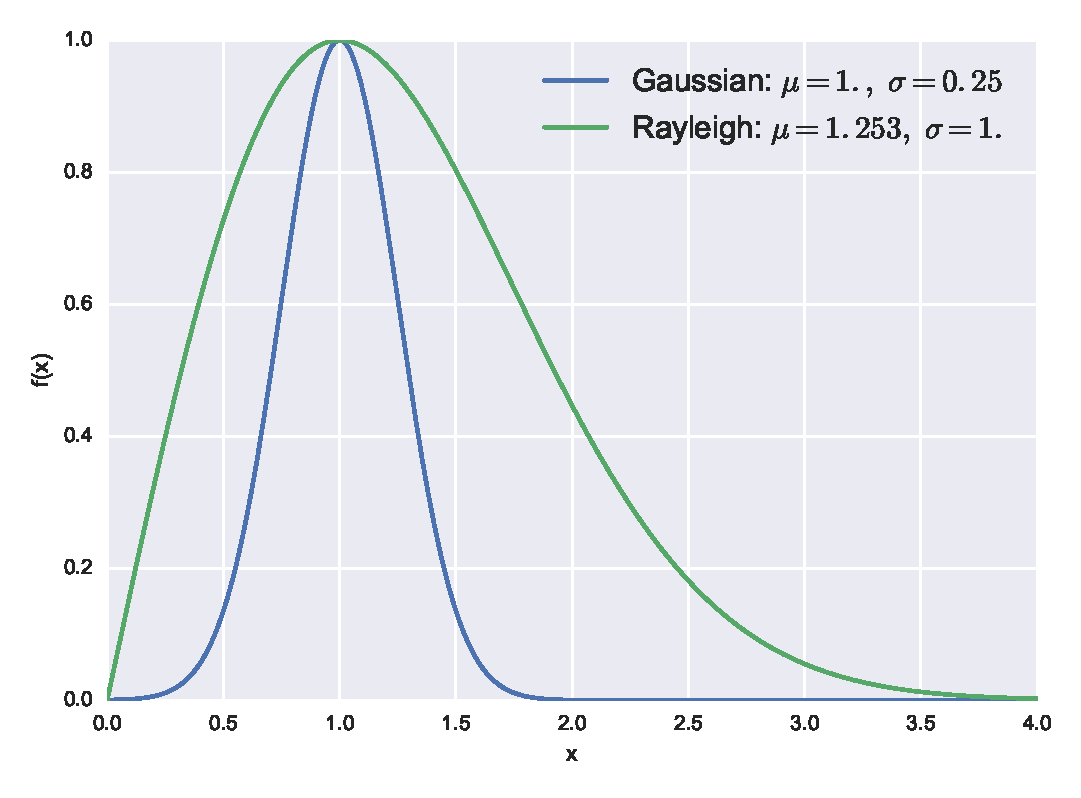
\includegraphics[width=0.7\linewidth]{3_review/figures/processing/pre-processing/noise/noisedistr.eps}
  \caption[Illustration of a Gaussian and Rayleigh distributions.]{Illustration
    of a Gaussian and Rayleigh distribution. Although the mode of these
    distributions are identical, it can be noted that the Rayleigh distribution
    ($\mu=1.253$) is suffering of a bias term when compared with the Gaussian
    distribution ($\mu=1$).}
  \label{fig:noisedistr}
\end{figure}

% Noise filtering
\item[] \textbf{Noise filtering}
The \ac{nmr} signal, measured and acquired in the k-space, is affected by noise.
This noise obeys a complex Gaussian white noise mainly due to thermal noises in
the patient~\cite{Nowak1999}.
Furthermore, \ac{mri} images visualized by radiologists are in fact the
magnitude images resulting from the complex Fourier transform of the k-space
data.
The complex Fourier transform does not affect the Gaussian noise
characteristics since this is a linear and orthogonal
transform~\cite{Nowak1999}.
However, the calculation of the magnitude is a non-linear transform --- i.e.,
the square root of the sum of squares of real and the imaginary parts ---
implying that the noise distribution is no longer Gaussian; it indeed follows a
Rician distribution making the denoising task more challenging.
Briefly, a Rician distribution is characterized as follows: in low-\ac{si}
region (low-\ac{snr}), it can be approximated with a Rayleigh distribution
while in high-\ac{si} region (high-\ac{snr}), it is similar to a Gaussian
distribution~\cite{Manjon2008}.
Refer to \acs{fig}\,\ref{fig:noisedistr} to observe the difference between a
Gaussian and a Rayleigh distribution.
Comprehensive reviews regarding denoising methods can be found
in~\cite{Buades2005,Mohan2014}.

Median filtering is the simplest approach used to address the denoising issue
in \ac{mri} images~\cite{Ozer2009,Ozer2010}.
In both studies, \citeauthor{Ozer2010}~\cite{Ozer2009,Ozer2010} used a
square-shaped kernel of size \SI[product-units=repeat]{5x5}{\px}.

More recently, \citeauthor{rampun2016quantitative} used a combination of median
and anisotropic diffusion
filter~\cite{rampun2015classifying,rampun2016computer,rampun2016computerb,rampun2016quantitative},
proposed in~\cite{ling2002smoothing}.
In low-\ac{snr} images, the gradient generated by an edge and noise can be
similar, making the denoising by diffusion more challenging.
In this condition, the threshold allowing to locally differentiate a noise
gradient from an edge gradient needs to be increased, at the cost of blurring
edges after filtering.
Therefore, \citeauthor{ling2002smoothing}~\cite{ling2002smoothing} proposed to
apply a standard anisotropic diffusion filter with a low threshold followed by
a median filtering to remove large noise spikes.



\citeauthor{samarasinghe2016semi} filtered \ac{dce}-\ac{mri} images with a
sliding 3D Gaussian filter~\cite{samarasinghe2016semi}.
However, from a theoretical point of view, this simple filtering method is not
well formalized to address the noise distribution in \ac{mri} images.
That is why more complex approaches have been proposed to overcome this problem.
Another common method used to denoise \ac{mri} images is based on wavelet
decomposition and shrinkage.
This filtering exploits the sparsity property of the wavelet decomposition.
The projection of a noisy signal from the spatial-domain to the wavelet-domain
implies that only few wavelet coefficients contribute to the ``signal-free
noise'' while all wavelet coefficients contribute to the
noise~\cite{Donoho1994}.
Therefore, insignificant wavelet coefficients are thresholded/attenuated to
enforce the sparsity in the wavelet-domain, which results to a denoising
process in the spatial domain.
Investigations focus on the strategies to perform the most adequate coefficient
shrinkage (e.g., thresholding, singularity property, or Bayesian
framework)~\cite{Pizurica2002}.
\citeauthor{Ampeliotis2008} denoised the magnitude \ac{mri}
images~\cite{Ampeliotis2007,Ampeliotis2008} --- i.e., \ac{t2w}-\ac{mri} and
\ac{dce}-\ac{mri} --- by wavelet shrinkage, using thresholding
techniques~\cite{Mallat2008}.
However, since the wavelet transform is an orthogonal transform, the Rician
distribution of the noise is preserved in the wavelet-domain.
Hence, for low-\ac{snr}, the wavelet and scaling coefficients still suffer from
a bias due to this specific noise distribution~\cite{Nowak1999}.
That is why, \citeauthor{Lopes2011} filtered \ac{t2w}-\ac{mri}
images~\cite{Lopes2011}, using the method proposed in~\cite{Pizurica2003} based
on joint detection and estimation theory.
In this approach, the wavelet coefficients ``free-of-noise'' are estimated from
the noisy wavelet coefficients using a \ac{map} estimate.
Furthermore, the designed estimator takes spatial context into account by
including both local and global information in the prior probabilities.
The different probabilities needed by the \ac{map} are empirically estimated by
using mask images, representing the locations of the significant wavelet
coefficients.
These mask images are computed by thresholding the detail images obtained from
the wavelet decomposition.
To remove the bias from the wavelet and scaling coefficients, the squared
magnitude \ac{mri} image is computed instead of the magnitude \ac{mri} image as
proposed in~\cite{Nowak1999}.
This involves changing the Rician distribution to a scaled non-central
Chi-squared distribution.
It implies that the wavelet coefficients are also unbiased estimators and the
scaling coefficients are unbiased estimators but up to a constant $C$ as
defined in \acs{eq}\,\eqref{eq:nowakC} which needs to be subtracted from each
scaling coefficient such as:

\begin{equation}
  C=2^{(J+1)}\hat{\sigma}^2 \ ,
  \label{eq:nowakC}
\end{equation}

\noindent where $J$ is the number of levels of the wavelet decomposition and
$\hat{\sigma}$ is an estimate of the noise standard deviation.

\begin{figure}
  \centering
  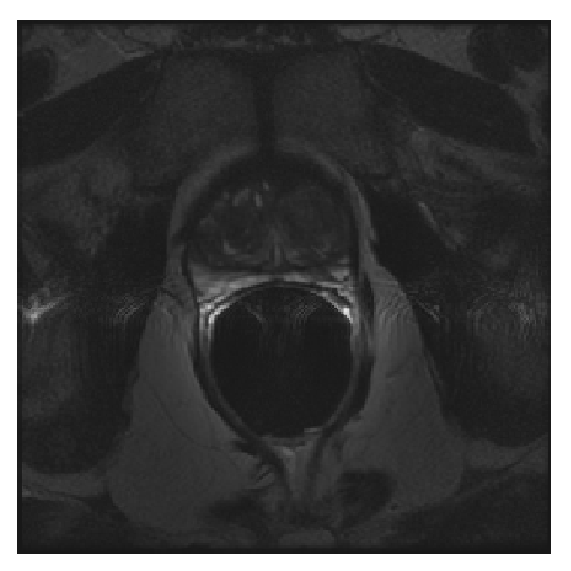
\includegraphics[width=0.3\linewidth]{3_review/figures/processing/pre-processing/bias/t2w_bias_antenna.eps}
  \caption[Non-homogeneity artifacts due to perturbation of the endorectal
  coil.]{Example of artifacts with high \acs*{si} due to perturbation from the
    endorectal coil which create non-homogeneity.}
  \label{fig:bias}
\end{figure}

% Artifacts filtering
\item[] \textbf{Bias correction}
Besides being corrupted by noise, \ac{mri} images are also affected by the
inhomogeneity of the \ac{mri} field commonly referred to as bias
field~\cite{Styner2000}.
This bias field results in a smooth variation of the \ac{si} through the image.
When an endorectal coil is used, a resulting artifact of an hyper-intense
signal is observed around the coil as depicted in \acs{fig}\,\ref{fig:bias}.
As a consequence, the \ac{si} of identical tissues varies depending on their
spatial location in the image making further processes such as segmentation,
registration, or classification more challenging~\cite{Jungke1987,Vovk2007}.
A comprehensive review of bias correction methods is proposed
in~\cite{Vovk2007}.

The model of image formation is usually formalized as:

\begin{equation}
  s(\mathbf{x}) = o(\mathbf{x})b(\mathbf{x}) + \eta(\mathbf{x}) \ ,
  \label{eq:biasmodel}
\end{equation}

\noindent where $s(\mathbf{x})$ is the corrupted \ac{si} at the pixel for the
image coordinates $\mathbf{x} = \{x,y\}$, $o(\mathbf{x})$ is the ``noise-free
signal'', $b(\mathbf{x})$ is the bias field function and $\eta(\mathbf{x})$ is
an additive white Gaussian noise.

Hence, the task of bias correction involves estimating the bias function
$b(\mathbf{x})$ in order to infer the ``signal-free bias'' $o(\mathbf{x})$.

\citeauthor{Viswanath2009} corrected this artifact on \ac{t2w}-\ac{mri}
images~\cite{Viswanath2009}, using the model proposed in~\cite{Styner2000}, in
which \citeauthor{Styner2000} model the bias field function by using a linear
combination of Legendre polynomials $f_i$ as:

\begin{align}
  \hat{b}(\mathbf{x},\mathbf{p}) & = \sum_{i=0}^{m-1} p_i f_i(\mathbf{x}) \\
  \nonumber
                                 & =  \sum_{i=0}^{l} \sum_{j=0}^{l-i} p_{ij}
                                   P_i(x) P_j(y) \ ,
                                   \label{eq:biascorr}
\end{align}

\noindent where $\hat{b}(\cdot)$ is the bias estimation with the image
coordinates $\mathbf{x} = \{x,y\}$ and the $m$ coefficients of the linear
combination $\mathbf{p} = {p_{11},\dotsc,p_{ij}}$; $m$ can be defined as
$m=(l+1)\frac{(l+2)}{2}$ where $l$ is the degree of Legendre polynomials chosen
and $P_i(\cdot)$ denotes a Legendre polynomial of degree $i$.

This family of functions offers to model the bias function as a smooth
inhomogeneous function across the image.
To estimate the set of parameters $\mathbf{p}$, a cost function is defined
which relies on the following assumptions: (i) an image is composed of $k$
regions with a mean $\mu_k$ and a variance $\sigma^{2}_{k}$ for each particular
class, and (ii) each noisy pixel belongs to one of the $k$ regions with its
\ac{si} value close to the class mean $\mu_k$.
Hence, the cost function is defined as:

\begin{equation}
  C(\mathbf{p}) = \sum_{\mathbf{x}} \prod_{k} \rho_k(s(\mathbf{x}) -
  \hat{b}(\mathbf{x},\mathbf{p}) - \mu_k) \ ,
  \label{eq:costbias}
\end{equation}

\begin{equation}
  \rho_k(x) = \frac{x^2}{x^2 + 3 \sigma_k^2} \ ,
  \label{eq:mestbias}
\end{equation}

\noindent where $\rho_k(\cdot)$ is a M-estimator allowing estimations to be
less sensitive to outliers than the usual squared distance~\cite{Li1996}.

Finally, the parameters $\mathbf{p}$ are estimated by finding the minimum of
the cost function $C(\mathbf{p})$, which was optimized using the non-linear
$(1+1)$ \ac{es} optimizer~\cite{Styner1997}.

In a later publication, \citeauthor{Viswanath2012}~\cite{Viswanath2012} as well
as \citeauthor{giannini2015fully}~\cite{giannini2015fully} corrected
\ac{t2w}-\ac{mri} using the well known N3 algorithm~\cite{Sled1998} in which
\citeauthor{Sled1998} infer the bias function using the \acp{pdf} of the signal
and bias.
Taking advantage of the logarithm property, the model in
\acs{eq}\,\eqref{eq:biasmodel} becomes additive as expressed in
\acs{eq}\,\eqref{eq:logbias}.

\begin{eqnarray}
  \log s(\mathbf{x}) & = & \log b(\mathbf{x}) + \log \left( o(\mathbf{x}) +
                           \frac{\eta(\mathbf{x})}{b(\mathbf{x})} \right) \ ,
                           \nonumber \\
                     & \approx & \log b(\mathbf{x}) + \log \hat{o}(\mathbf{x})
                                 \ , \label{eq:logbias}
\end{eqnarray}

\noindent where $\hat{o}(\mathbf{x})$ is the signal only degraded by
noise. \citeauthor{Sled1998} show that \acs{eq}\,\eqref{eq:logbias} is related
to \acp{pdf} such that:

\begin{equation}
  S(s) = B(s) * O(s) \ ,
  \label{eq:distrbias}
\end{equation}

\noindent where $S(\cdot)$, $B(\cdot)$, and $O(\cdot)$ are the \acp{pdf} of
$s(\cdot)$, $b(\cdot)$, and $o(\cdot)$, respectively.

The corrupted signal $s$ is restored by finding the multiplicative field $b$
which maximizes the frequency content of the distribution $O$.
\citeauthor{Sled1998}~\cite{Sled1998} argued that a brute-force search through
all possible fields $b$ and selecting the one which maximizes the high
frequency content of $O$ is possible but far too complex.
By assimilating the bias field distribution to be a near Gaussian distribution
as \textit{a priori}, it is then possible to infer the distribution $O$ using
the Wiener deconvolution given $B$ and $S$ and later estimate the corresponding
smooth field $b$.

\citeauthor{Lv2009} corrected the non-homogeneity in \ac{t2w}-\ac{mri}
images~\cite{Lv2009} by using the method proposed in~\cite{Madabhushi2006}.
\citeauthor{Madabhushi2006}~\cite{Madabhushi2006} proposed to correct the
\ac{mri} images by detecting the image foreground via \ac{gscale} in an
iterative manner and estimating a bias field function based on a
2\textsuperscript{nd} order polynomial model.
First, the background of the \ac{mri} image is eliminated by thresholding, in
which the threshold value is commonly equal to the mean \ac{si} of the
considered image.
Then, a seeded region growing algorithm is applied in the image foreground,
considering every thresholded pixel as a potential seed.
However, pixels already assigned to a region are not considered any more as a
potential seed.
As in seeded region growing algorithm~\cite{Shapiro2001}, two criteria are
taken into account to expand a region.
First, the region grows using a connected-neighbourhood, initially defined by
the user.
Then, the homogeneity of \ac{si} is based on a fuzzy membership function taking
into account the absolute difference of two pixel \ac{si}.
Depending on the membership value --- corresponding to a threshold which needs
to be defined --- the pixel considered is merged or not to the region.
Once this segmentation is performed, the largest region $R$ is used as a mask
to select pixels of the original image and the mean \ac{si}, $\mu_{R}$, is
computed.
The background variation $b(\mathbf{x})$ is estimated as:

\begin{equation}
  b(\mathbf{x}) = \frac{s(\mathbf{x})}{\mu_{R}}, \ \forall \mathbf{x} \in R \ ,
  \label{eq:backest}
\end{equation}

\noindent where $s(\mathbf{x})$ is the original \ac{mri} image.

Finally, a 2\textsuperscript{nd} order polynomial
$\hat{b}_{\Theta}(\mathbf{x})$ is fitted in a least-squares sense as in
\acs{eq}\,\eqref{eq:lsolv},

\begin{equation}
  \hat{\Theta} = \argmin_{\Theta} | b(\mathbf{x}) -
  \hat{b}_{\Theta}(\mathbf{x}) |^{2}, \ \forall \mathbf{x} \in R \ .
  \label{eq:lsolv}
\end{equation}

Finally, the whole original \ac{mri} image is corrected by dividing it by the
estimated bias field function $\hat{b}_{\Theta}(\mathbf{x})$.
The convergence is reached when the number of pixels in the largest region $R$
does not change significantly between two iterations.

\item[] \textbf{\Ac{si} normalization/standardization}
As discussed in the later section, segmentation or classification tasks are
usually composed of a learning stage using a set of training patients.
Hence, one can emphasize the desire to perform automatic diagnosis with a high
repeatability or in other words, one would ensure to obtain consistent \ac{si}
of tissues across patients of the same group --- i.e., healthy patients
\textit{vs.} patients with \ac{cap} --- for each \ac{mri} modality.
However, it is a known fact that variability between patients occurs during the
\ac{mri} examinations even using the same scanner, protocol or sequence
parameters~\cite{Nyul1999}.
Hence, the aim of normalization or standardization of the \ac{mri} data is to
remove the variability between patients and enforce the repeatability of the
\ac{mri} examinations.
These standardization methods are categorized either as statistical-based
standardization or organ \ac{si}-based standardization.

\citeauthor{Artan2010}~\cite{Artan2009,Artan2010},
\citeauthor{Ozer2010}~\cite{Ozer2009,Ozer2010}, and
\citeauthor{rampun2016quantitative}~\cite{,rampun2015classifying,rampun2015computer,rampun2016computer,rampun2016computerb,rampun2016quantitative}
standardized \ac{t2w}-\ac{mri}, \ac{dce}-\ac{mri}, and \ac{dw}-\ac{mri} images
by computing the \textit{standard score} (also called \textit{z-score}) of the
pixels of the \ac{pz} as:

\begin{equation}
  I_s(\mathbf{x}) = \frac{ I_r(\mathbf{x}) - \mu_{pz}}{\sigma_{pz}}, \ \forall
  \mathbf{x} \in \text{PZ} \ ,
  \label{eq:meansta}
\end{equation}

\noindent where $I_s(\mathbf{x})$ is the standardized \ac{si} with the image
coordinates $\mathbf{x} = \{x,y\}$, $I_r(\mathbf{x})$ is the raw \ac{si},
$\mu_{pz}$ is the mean \ac{si} of the \ac{pz} and $\sigma_{pz}$ is the \ac{si}
standard deviation in the \ac{pz}.
This transformation enforces the image \ac{pdf} to have a zero mean and a unit
standard deviation.
In a similar way, \citeauthor{Liu2013} normalized \ac{t2w}-\ac{mri} by making
use of the median and inter-quartile range for all the pixels~\cite{Liu2013}.

\citeauthor{lemaitre2016normalization} proposes to use the a priori that the
underlying data distribution follows a Rician distribution instead of a
Gaussian distribution~\cite{lemaitre2016normalization}.
The data are standardized by removing the mean and scaled it by dividing by the
standard-deviation which are empirically computed as follows:

\begin{equation}
  \mu_{r} = \sigma  \sqrt{\frac{\pi}{2}}\,\,L_{1/2}(-\frac{\nu^2}{2\sigma^2})  \ ,
  \label{eq:meanr}
\end{equation}

\begin{equation}
  \sigma_{r} = 2\sigma^2+\nu^2-\frac{\pi\sigma^2}{2}L_{1/2}^2\left(\frac{-\nu^2}{2\sigma^2}\right)  \ ,
  \label{eq:var}
\end{equation}

\noindent where $\nu$ and $\sigma$ are the distance between the reference point
and the center of the bivariate distribution and the scale, respectively;
$L_{1/2}$ denotes a Laguerre polynomial.

\citeauthor{Lv2009} scaled the \ac{si} of \ac{t2w}-\ac{mri} images using the
method proposed in~\cite{Nyul2000} based on \ac{pdf} matching~\cite{Lv2009}.
This approach is based on the assumption that \ac{mri} images from the same
sequence should share the same \ac{pdf} appearance.
Hence, one can approach this issue by transforming and matching the \acp{pdf}
using some statistical landmarks such as quantiles.
Using a training set, these statistical landmarks --- such as minimum,
25\textsuperscript{th} percentile, median, 75\textsuperscript{th} percentile,
and maximum --- are extracted for $N$ training images:

\begin{eqnarray}
  \Phi_{0} & = & \{ \phi_{0}^{1}, \phi_{0}^{2}, \cdots, \phi_{0}^{N} \} \ , \nonumber \\
  \Phi_{25} & = & \{ \phi_{25}^{1}, \phi_{25}^{2}, \cdots, \phi_{25}^{N} \} \ , \nonumber \\
  \Phi_{50} & = & \{ \phi_{50}^{1}, \phi_{50}^{2}, \cdots, \phi_{50}^{N} \} \ ,  \label{eq:quantileStd} \\
  \Phi_{75} & = & \{ \phi_{75}^{1}, \phi_{75}^{2}, \cdots, \phi_{75}^{N} \} \ , \nonumber \\
  \Phi_{100} & = & \{ \phi_{100}^{1}, \phi_{100}^{2}, \cdots, \phi_{100}^{N} \} \ , \nonumber
\end{eqnarray}

\noindent where $\phi_{n^\text{th}}^{i^{\text{th}}}$ is the $n^{\text{th}}$
percentile of the $i^{\text{th}}$ training image.

\citeauthor{lemaitre2016normalization} extended the use of non-parametric
transformation using an elastic transformation instead of a piecewise-linear
transformation~\cite{lemaitre2016normalization}.
They proposed to use a generic method to register functional data based on the
\ac{srsf} representation~\cite{Srivastava2011} which transforms the
Fisher-Rao metric into the conventional $\mathbb{L}^2$ metric, and thus allows
to define a cost function corresponding to an Euclidean distance between two
functions in this new representation.

\begin{figure}
  \centering
  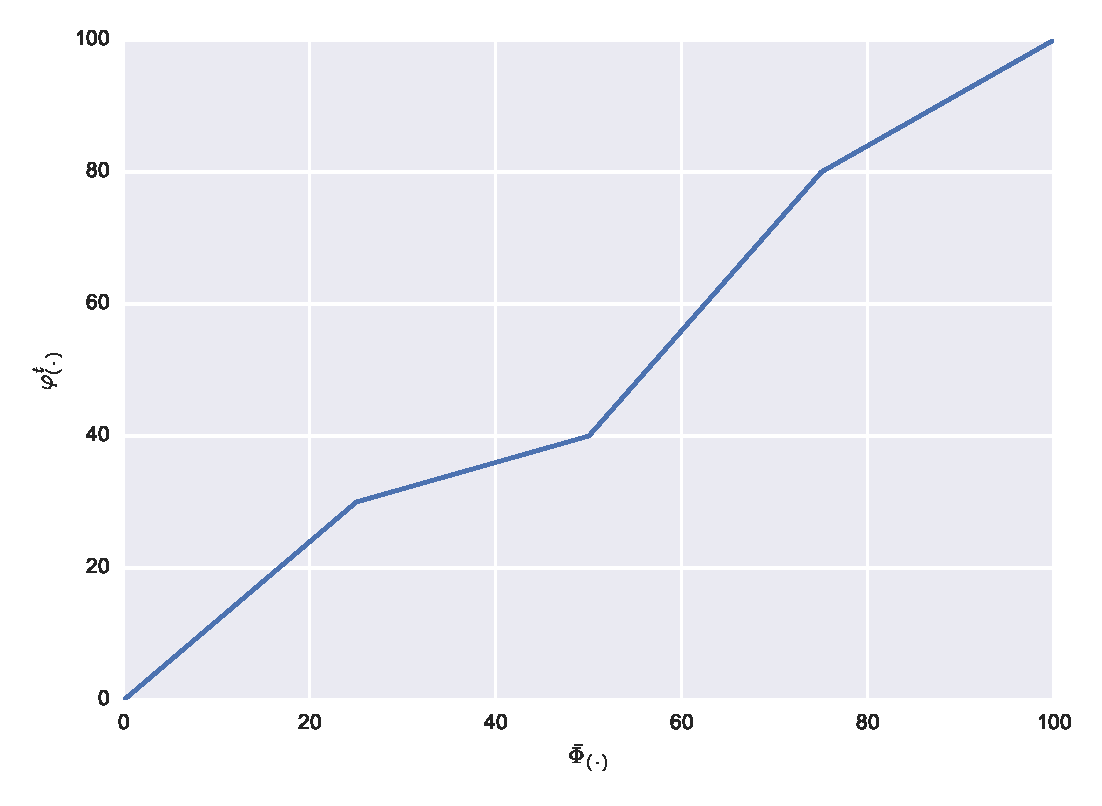
\includegraphics[width=0.7\linewidth]{3_review/figures/processing/pre-processing/normalization/linear_transform_parts.eps}
  \caption{Example of piecewise linear normalization as proposed
    in~\cite{Nyul2000}.}
  \label{fig:imnorm}
\end{figure}

Then, the mean of each statistical landmarks $\{ \bar{\Phi}_{0},
\bar{\Phi}_{25}, \bar{\Phi}_{50}, \bar{\Phi}_{75}, \bar{\Phi}_{100} \}$ is also
calculated.
Once this training stage is performed, a piecewise linear transformation
$\mathcal{T}(\cdot)$ is computed as in \acs{eq}\,\eqref{eq:linearMap}.
For each test image $t$, this transformation maps each statistical landmark
$\varphi_{(\cdot)}̂^{t}$ of the image $t$ to the pre-learned statistical
landmarks $\bar{\Phi}_{(\cdot)}$.
An example of such piecewise linear function is depicted in
\acs{fig}\,\ref{fig:imnorm}.

\begin{equation}
  \small
  \mathcal{T}(s(\mathbf{x})) =
  \begin{cases}
    \lceil \bar{\Phi}_{0}+( s(\mathbf{x}) - \varphi_{0}^{t} ) \left(
      \frac{\bar{\Phi}_{25} - \bar{\Phi}_{0}}{\varphi_{25}^{t} -
        \varphi_{0}^{t}} \right) \rceil \ , & \text{if $\varphi_{0}^{t} \leq
      s(\mathbf{x})<\varphi_{25}^{t})$} \ , \\
    \lceil \bar{\Phi}_{25}+( s(\mathbf{x}) - \varphi_{25}^{t} ) \left(
      \frac{\bar{\Phi}_{50} - \bar{\Phi}_{25}}{\varphi_{50}^{t} -
        \varphi_{25}^{t}} \right) \rceil \ , & \text{if $\varphi_{25}^{t} \leq
      s(\mathbf{x})<\varphi_{50}^{t})$} \ , \\
    \lceil \bar{\Phi}_{50}+( s(\mathbf{x}) - \varphi_{50}^{t} ) \left(
      \frac{\bar{\Phi}_{75} - \bar{\Phi}_{50}}{\varphi_{75}^{t} -
        \varphi_{50}^{t}} \right) \rceil \ , & \text{if $\varphi_{50}^{t} \leq
      s(\mathbf{x})<\varphi_{75}^{t})$} \ , \\
    \lceil \bar{\Phi}_{75}+( s(\mathbf{x}) - \varphi_{75}^{t} ) \left(
      \frac{\bar{\Phi}_{100} - \bar{\Phi}_{75}}{\varphi_{100}^{t} -
        \varphi_{75}^{t}} \right) \rceil \ , & \text{if $\varphi_{75}^{t} \leq
      s(\mathbf{x})\leq \varphi_{100}^{t})$} \ ,
  \end{cases}
  \label{eq:linearMap}
\end{equation}

\citeauthor{Viswanath2012} used a variant of the piecewise linear normalization
presented in~\cite{Madabhushi2006a}, to standardize \ac{t2w}-\ac{mri}
images~\cite{Viswanath2009,Viswanath2011,Viswanath2012}.
Instead of computing the \ac{pdf} of an entire image, a pre-segmentation of the
foreground is carried out via \ac{gscale} which has been discussed in the bias
correction section.
Once the foreground is detected, the largest region is extracted, and the
regular piecewise linear normalization is applied.

\begin{figure}
  \centering
  \hspace*{\fill}
  \subfloat[Illustration and location of the bladder on a \ac{t2w}-\ac{mri}
  image acquired with a \SI{3}{\tesla} \ac{mri} scanner]{\label{subfig:bladder}
    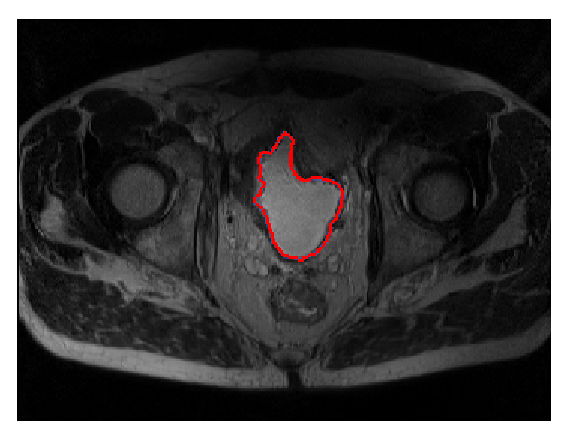
\includegraphics[width=0.3\linewidth]{3_review/figures/processing/pre-processing/niaf/t2w_bladder.eps}}
  \hfill
  \subfloat[Illustration and location of the femoral arteries on a
  \ac{t1w}-\ac{mri} image acquired with a \SI{3}{\tesla} \ac{mri}
  scanner]{\label{subfig:arteries}
    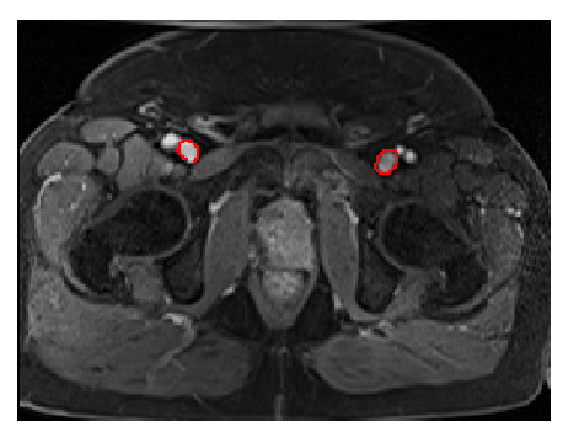
\includegraphics[width=0.3\linewidth]{3_review/figures/processing/pre-processing/niaf/t1w_arteries.eps}}
  \hspace*{\fill}
  \caption{Illustration of the two organs used in~\cite{Niaf2011,Niaf2012} to
    normalize \acs*{t2w}-\acs*{mri} and \acs*{t1w}-\acs*{mri} images.}
  \label{fig:niaf}
\end{figure}

The standardization problem can be tackled by normalizing the MRI images using
the \ac{si} of some known organs present in these images.
\citeauthor{Niaf2012} and \citeauthor{lehaire2014computer} normalized
\ac{t2w}-\ac{mri} images by dividing the original \ac{si} of the images by the
mean \ac{si} of the bladder~\cite{Niaf2011,Niaf2012,lehaire2014computer}, which
is depicted in \acs{fig}\,\ref{subfig:bladder}.
\citeauthor{giannini2015fully} also normalized the same modality but using the
signal intensity of the obturator muscle~\cite{giannini2015fully}.
Likewise, \citeauthor{Niaf2011} standardized the \ac{t1w}-\ac{mri} images using
the \ac{aif}~\cite{Niaf2011}.
They computed the \ac{aif} by taking the mean of the \ac{si} in the most
enhanced part of the common femoral arteries --- refer to
\acs{fig}\,\ref{subfig:arteries} --- as proposed in~\cite{Wiart2007}.
Along the same line, \citeauthor{samarasinghe2016semi} normalized the \ac{si}
of lesion regions in \ac{t1w}-\ac{mri} using the mean intensity of the prostate
gland in the same modality~\cite{samarasinghe2016semi}.

\end{enumerate}

\subsubsection{\acs*{mrsi} modalities}\label{subsubsec:ch3:mriprepro}

As presented in \acs{sec}\,\ref{subsec:chp2:imaging:mrsi}, \ac{mrsi} is a
modality related to a one dimensional signal.
Hence, specific pre-processing steps for this type of signals have been applied
instead of standard signal processing methods.

\setenumerate{listparindent=\parindent,itemsep=10px}
\setlist{noitemsep}
\begin{enumerate}[leftmargin=*]

\begin{figure}
  \centering
  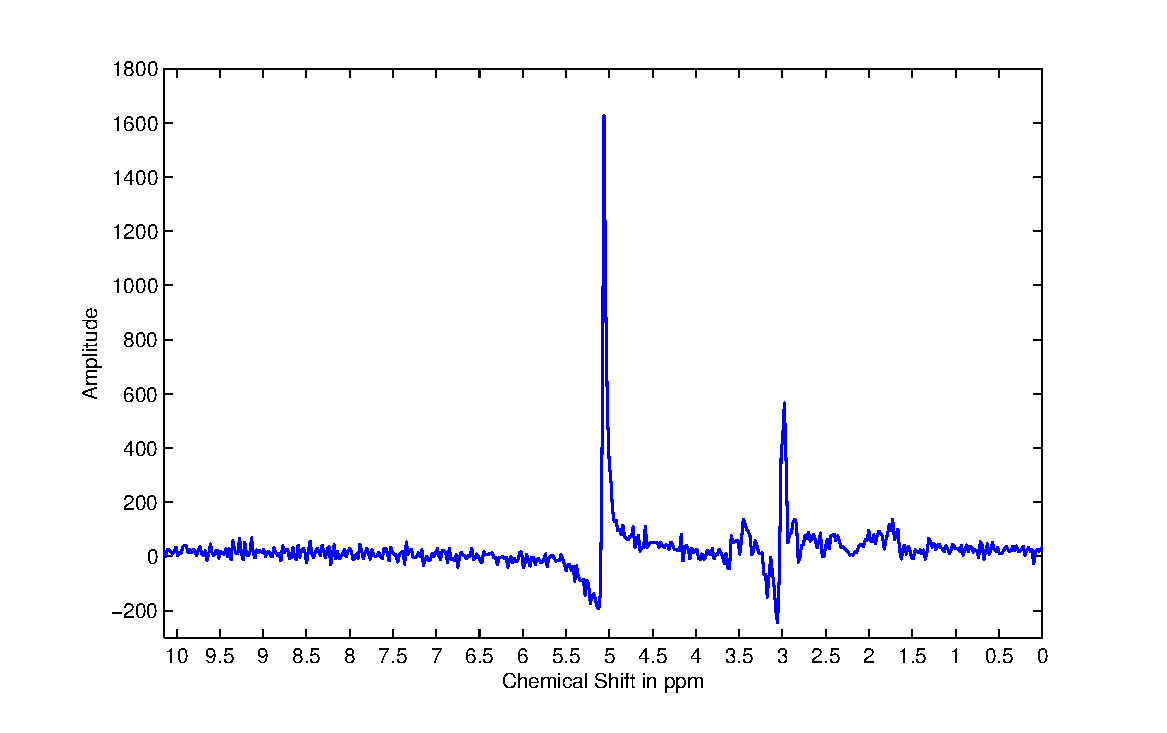
\includegraphics[width=0.7\linewidth]{3_review/figures/processing/pre-processing/phase/phase.eps}
  \caption[Illustration of phase malignant in an \acs*{mrsi}
  spectra.]{Illustration of phase misalignment in an \acs*{mrsi} spectra
    acquired with a \SI{3}{\tesla} \acs*{mrsi} scanner. Note the distortion of
    the signal specially visible for the water and citrate peaks visible at
    \SI{5}{\ppm} and \SI{3}{\ppm}, respectively}
  \label{fig:phase}
\end{figure}

\item[] \textbf{Phase correction}
Acquired \ac{mrsi} spectra suffer from zero-order and first-order phase
misalignment~\cite{Chen2002,Osorio-Garcia2012} as depicted in
\acs{fig}\,\ref{fig:phase}.
\citeauthor{Parfait2012} and \citeauthor{trigui2017automatic} used a method
proposed by \citeauthor{Chen2002} where the phase of \ac{mrsi} signal is
corrected based on entropy minimization in the frequency
domain~\cite{Parfait2012,trigui2016classification,trigui2017automatic}.
The corrected \ac{mrsi} signal $o(\xi)$ can be expressed as:

\begin{eqnarray}
  \Re(o(\xi)) & = & \Re(s(\xi))\cos(\Phi(\xi)) - \Im(\xi)\sin(\Phi(\xi)) \ ,
                    \nonumber  \\
  \Im(o(\xi)) & = & \Im(s(\xi))\cos(\Phi(\xi)) + \Re(\xi)\sin(\Phi(\xi)) \ ,
                    \nonumber \\
  \Phi(\xi) & = & \phi_0 + \phi_1 \frac{\xi}{N} \ , \label{eq:mrsiphcorr}
\end{eqnarray}

\noindent where $\Re(\cdot)$ and $\Im(\cdot)$ are the real and imaginary part
of the complex signal, respectively, $s(\xi)$ is the corrupted \ac{mrsi}
signal, $\phi_0$ and $\phi_1$ are the zero-order and first-order phase
correction terms respectively and $N$ is the total number of samples of the
\ac{mrsi} signal.

\citeauthor{Chen2002} tackled this problem as an optimization in which $\phi_0$
and $\phi_1$ have to be inferred.
Hence, the simplex Nelder-Mead optimizer~\cite{Nelder1965} is used to minimize
the following cost function based on the \textit{Shannon entropy} formulation:

\begin{equation}
  \hat{\Phi} = \argmin_{\Phi} \left[ - \sum \Re(s'(\xi)) \ln \Re(s'(\xi)) +
    \lambda \|\Re(s(\xi))\|_2 \right] \ ,
  \label{eq:phcost}
\end{equation}

\noindent where $s'(\xi)$ is the first derivative of the corrupted signal
$s(\xi)$ and $\lambda$ is a regularization parameter.
Once the best parameter $\Phi$ vector is obtained, the \ac{mrsi} signal is
corrected using \acs{eq}\,\eqref{eq:mrsiphcorr}.

\begin{figure}
  \centering
  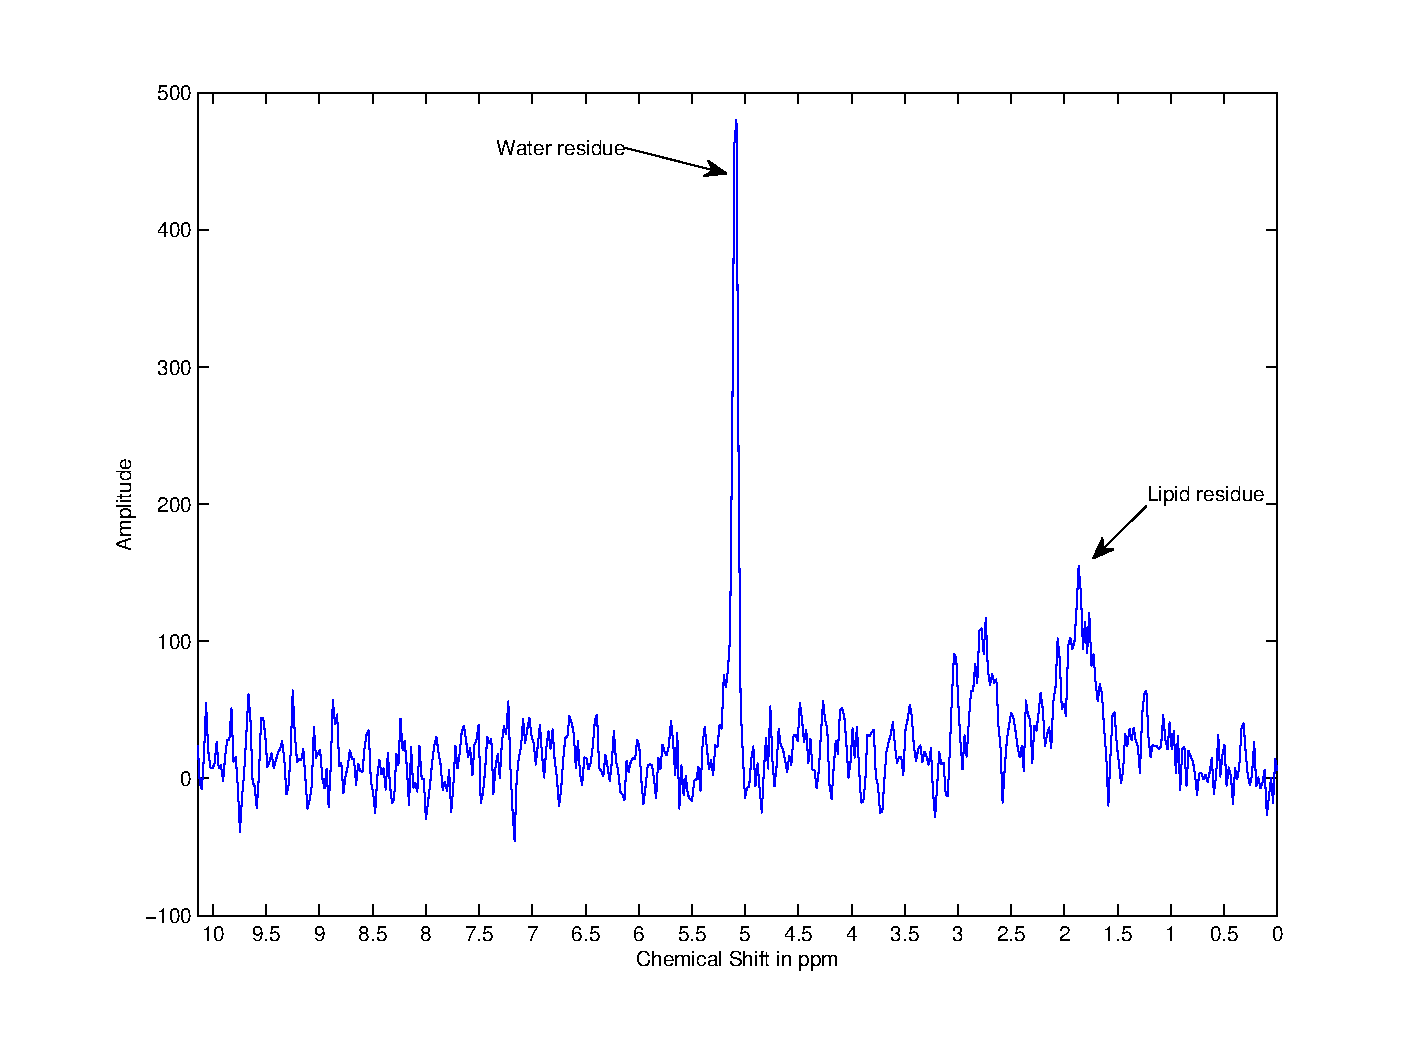
\includegraphics[width=0.7\linewidth]{3_review/figures/processing/pre-processing/water/water_fat.eps}
  \caption[Illustration of water and fat residues in \acs*{mrsi} signal after
  suppression during acquisition.]{Illustration of the residues of water and
    fat even after their suppression during the acquisition protocol. The
    acquisition has been carried out with a \SI{3}{\tesla} \acs*{mri}.}
  \label{fig:waterfat}
\end{figure}

\item[] \textbf{Water and lipid residuals filtering}
The water and lipid metabolites occur in much higher concentrations than the
metabolites of interest, namely choline, creatine, and
citrate~\cite{Zhu2010,Osorio-Garcia2012}.
Fortunately, specific \ac{mrsi} sequences have been developed in order to
suppress water and lipid metabolites using pre-saturation
techniques~\cite{Zhu2010}.
However, these techniques do not perfectly remove water and lipids peaks and
some residuals are still present in the \ac{mrsi} spectra as illustrated in
\ac{fig}\,\ref{fig:waterfat}.
Therefore, different post-processing methods have been proposed to enhance the
quality of the \ac{mrsi} spectra by removing these residuals.
For instance, \citeauthor{Kelm2007}~\cite{Kelm2007} used the HSVD algorithm
proposed by \citeauthor{Pijnappel1992}~\cite{Pijnappel1992} which models the
\ac{mrsi} signal by a sum of exponentially damped sine waves in the time domain
as \acs{eq}\,\eqref{eq:fidsig}.

\begin{equation}
  s(t) = \sum_{k=1}^{K} a_{k}\exp(i \phi_k) \exp( -d_{k} + i 2 \pi f_{k} ) t +
  \eta(t) \ ,
  \label{eq:fidsig}
\end{equation}

\noindent where $a_k$ is the amplitude proportional to the metabolite
concentration with a resonance frequency $f_{k}$, $d_k$ represents the damping
factor of the exponential, $\phi_k$ is the first-order phase, and $\eta(t)$ is
a complex white noise.

The ``noise-free signal'' can be found using the \ac{svd}
decomposition~\cite{Pijnappel1992}.
Therefore, the noisy signal is reorganized inside a Hankel matrix $H$.
It can be shown that the signal is considered as a ``noise-free signal'' if the
rank of $H$ is equal to rank $K$.
However, due to the presence of noise, $H$ is in fact a full rank matrix.
Thus, to recover the ``noise-free signal'', the rank of $H$ is truncated to $K$
using its \ac{svd} decomposition.
Hence, knowing the cut off frequencies of water --- i.e., \SI{4.65}{\ppm} ---
and lipid --- i.e., \SI{2.2}{\ppm} --- metabolites, their corresponding peaks
are reconstructed and subtracted from the original signal~\cite{Laudadio2002}.

\item[] \textbf{Baseline correction}
Sometimes, the problem discussed in the above section regarding the lipid
molecules is not addressed simultaneously with water residuals suppression.
Lipids and macro-molecules are known to affect the baseline of the \ac{mrsi}
spectra, causing errors while quantifying metabolites, especially the citrate
metabolite.

\citeauthor{Parfait2012} made the comparison of two different methods to detect
the baseline and correct the \ac{mrsi} spectra~\cite{Parfait2012} which are
based on~\cite{Lieber2003,Devos2004}.
\citeauthor{Lieber2003} corrected the baseline in the frequency domain by
fitting a low degree polynomial $p(x)$ --- e.g., 2\textsuperscript{nd} or
3\textsuperscript{rd} degree --- to the \ac{mrsi} signal $s(x)$ in a
least-squares sense~\cite{Lieber2003}.
Then, the values of the fitted polynomial are re-assigned as:

\begin{equation}
  p_f(x) =
  \begin{cases}
    p(x) \ , & \text{if $p(x) \leq s(x)$} \ , \\
    s(x) \ , & \text{if $p(x) > s(x)$} \ . \\
  \end{cases}
  \label{eq:lieber}
\end{equation}

Finally, this procedure of fitting and re-assignment is repeated on $p_f(x)$
until a stopping criterion is reached.
The final polynomial function is subtracted from the original signal $s(x)$ to
correct it.
\citeauthor{Parfait2012}~\cite{Parfait2012} modified this algorithm by
convolving a Gaussian kernel to smooth the \ac{mrsi} signal instead of fitting
a polynomial function, keeping the rest of the algorithm identical.
Unlike~\citeauthor{Lieber2003}~\cite{Lieber2003},
\citeauthor{Devos2004}~\cite{Devos2004} corrected the baseline in the time
domain by multiplying the \ac{mrsi} signal by a decreasing exponential function
as:

\begin{equation}
  c(t) = \exp (- \beta t) \ ,
  \label{eq:devos}
\end{equation}

\noindent with a typical $\beta$ value of $0.15$.
However, \citeauthor{Parfait2012} concluded that the method proposed
in~\cite{Lieber2003} outperformed the one in~\cite{Devos2004}.
The later study of \citeauthor{trigui2017automatic} used this conclusion and
adopted the same method~\cite{trigui2016classification,trigui2017automatic}.

The previous baseline correction methods does not provide an optimal solution
since the iterative low-pass filter enforces too much the smoothness of the
baseline.
\citeauthor{xi2008baseline} proposed a baseline detection derived from a
parametric smoothing model~\cite{xi2008baseline}.
The \ac{nmr} signal is formalized as a sum of a pure signal, the baseline
function, and an additive Gaussian noise such as:

\begin{equation}
  y_i = b_i + \mu_i e^{n_i} + \varepsilon_i \ ,
  \label{eq:methodBaselineDetectionModel}
\end{equation}

\noindent where $y_i$ is the \ac{nmr} signal, $b_i$ is the baseline, $\mu_i$ is
the true signal, and $n_i$ and $\varepsilon_i$ are Gaussian noises.

\citeauthor{xi2008baseline} propose to find the baseline function through an
iterative optimization by maximizing the following cost function:

\begin{equation}
  F(b) = \sum_{i = 1}^{N} b_i - \frac{A^{*} N^4}{\sigma} \sum_{i = 1}^{N} (b_{i+1} + b_{i-1} - 2 b_i)^2 - \frac{1.25 B^{*}}{\sigma} \sum_{i = 1}^{N} (b_i - \gamma_i)^2 g(b_i - \gamma_i) \ ,
  \label{eq:methodBaselineDetectionCostFunction}
\end{equation}

\noindent where $g(b_i - \gamma_i)$ is the Heaviside function, $A^*$ and $B^*$
are the terms controlling the smoothness and negative penalties, respectively,
$\sigma$ is an estimation of the standard deviation of the noise, and $N$ is
the total number of points in the \ac{mrsi} signal.

The standard deviation of the noise $\sigma$ is estimated as
in~\cite{xi2008baseline}, and the $A^{*}$ and $B^{*}$ are empirically set to $5
\times 10^{-6}$ and $100$, respectively, for all the \ac{mrsi} signal.
This method was used in the work of
\citeauthor{Lemaitre2016thesis}~\cite{Lemaitre2016thesis}.

In the contemporary work of \citeauthor{Tiwari2012}~\cite{Tiwari2012}, the
authors detected the baseline using a local non-linear fitting method avoiding
regions with significant peaks, which have been detected using an
experimentally parametric signal-to-noise ratio set to a value larger than
\SI{5}{\decibel}.

\begin{figure}
  \centering
  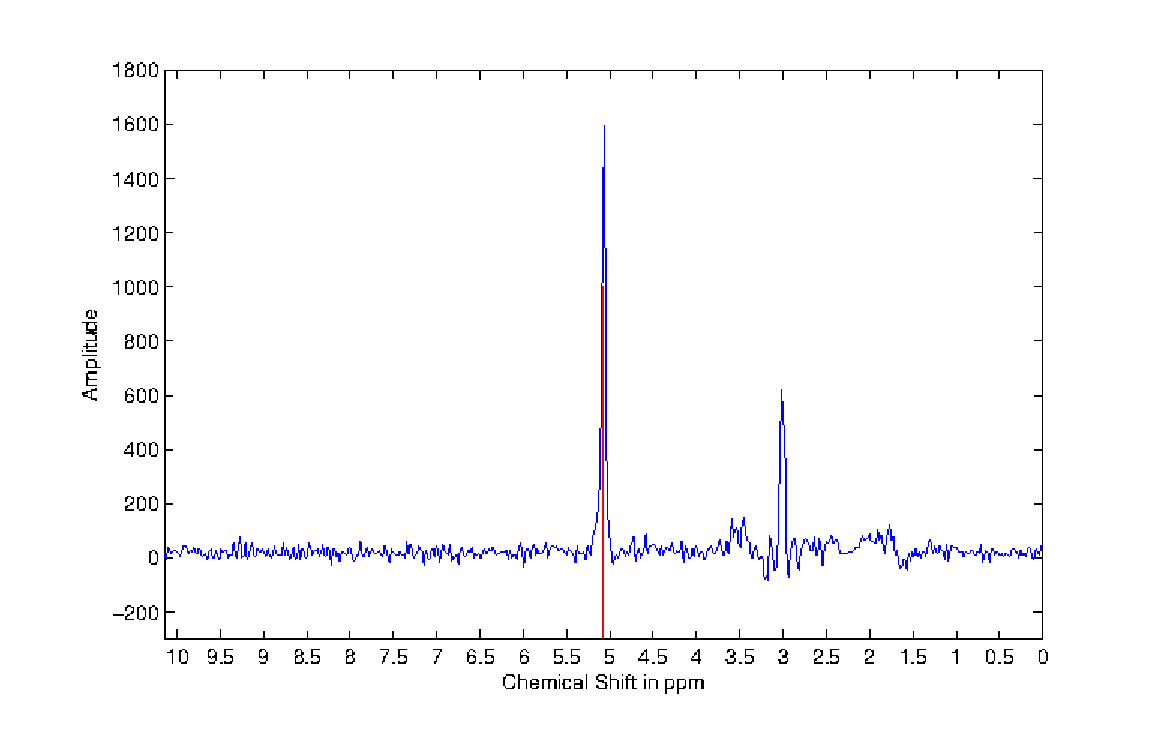
\includegraphics[width=0.7\linewidth]{3_review/figures/processing/pre-processing/frequency/frequency.eps}
  \caption[Illustration of frequency misalignment in a \acs*{mrsi}
  spectra.]{Illustration of frequency misalignment in a \acs*{mrsi} spectra
    acquired with a \SI{3}{\tesla} \acs*{mrsi} scanner. The water peak is known
    to be aligned at \SI{4.65}{\ppm}. However, it can be seen that the peak on
    this spectra is aligned at around \SI{5.1}{\ppm}.}
  \label{fig:frequency}
\end{figure}

\item[] \textbf{Frequency alignment}
Due to variations of the experimental conditions, a frequency shift is commonly
observed in the \ac{mrsi} spectra~\cite{Chen2002,Osorio-Garcia2012} as depicted
in \acs{fig}\,\ref{fig:frequency}.
\citeauthor{Tiwari2012}~\cite{Tiwari2012} corrected this frequency shift by
first detecting known metabolite peaks such as choline, creatine, or citrate
and minimizing the frequency error between the experimental and theoretical
values for each of these peaks~\cite{Tiwari2012}.

\item[] \textbf{Normalization}
The \ac{nmr} spectra is subject to variations due to intra-patient variations
and non homogeneity of the magnetic field.
\citeauthor{Parfait2012} as in~\cite{Devos2004} compared two methods to
normalize \ac{mrsi} signal~\cite{Parfait2012}.
In each method, the original \ac{mrsi} spectra is divided by a normalization
factor, similar to the intensity normalization described earlier.
The first approach consists in estimating the water concentration from an
additional \ac{mrsi} sequence where the water has not been suppressed.
The estimation is performed using the previously HSVD algorithm.
The second approach does not require any additional acquisition and is based on
the L$_2$ norm of the \ac{mrsi} spectra $\|s(\xi)\|_2$.
It should be noted that both \citeauthor{Parfait2012} and
\citeauthor{Devos2004} concluded that the L$_2$ normalization is the most
efficient method~\cite{Parfait2012}.
Lately, \citeauthor{trigui2017automatic} used the L$_2$ normalization in their
framework~\cite{trigui2016classification,trigui2017automatic}.

\end{enumerate}

\subsubsection{Summary}

The different pre-processing methods are summarized in \acs{tab}~\ref{tab:summary-preproc}.

\begin{table}
  \caption{Overview of the pre-processing methods used in \acs*{cad} systems.}
  \centering
  \begin{tabular}{l r}
    \toprule
    \textbf{Pre-processing operations} & \textbf{References} \\
    \midrule
    \textbf{\ac{mri} pre-processing:} & \\
    \quad Noise filtering: &  \\
    \quad \quad $\bullet$ Anisotropic median-diffusion filtering &
                                                                   \cite{rampun2015classifying,rampun2015computer,rampun2016computer,rampun2016computerb,rampun2016quantitative}
    \\
    \quad \quad $\bullet$ Gaussian filtering & \cite{samarasinghe2016semi}  \\
    \quad \quad $\bullet$ Median filtering & \cite{Ozer2009,Ozer2010}  \\
    \quad \quad $\bullet$ Wavelet-based filtering &
                                                    \cite{Ampeliotis2007,Ampeliotis2008,Lopes2011}
    \\ \\ [-1.5ex]
    \quad Bias correction: & \\
    \quad \quad $\bullet$ Parametric methods &
                                               \cite{Lv2009,Viswanath2009,giannini2015fully}
    \\
    \quad \quad $\bullet$ Non-parametric methods & \cite{Viswanath2011} \\ \\
    [-1.5ex]
    \quad Standardization: & \\
    \quad \quad $\bullet$ Statistical-based normalization: &
                                                             \cite{Artan2009,Artan2010,Lv2009,Ozer2009,Ozer2010,rampun2015classifying,rampun2015computer,rampun2016computer,rampun2016computerb,rampun2016quantitative,Viswanath2009,Viswanath2011,Viswanath2012,Lemaitre2016thesis}
    \\
    \quad \quad $\bullet$ Organ \ac{si}-based normalization &
                                                              \cite{Niaf2011,Niaf2012,lehaire2014computer,samarasinghe2016semi}
    \\ \\ [-1.5ex]
    \textbf{\ac{mrsi} pre-processing:} & \\ \\ [-1.5ex]
    \quad Phase correction &
                             \cite{Parfait2012,trigui2016classification,trigui2017automatic,Lemaitre2016thesis}
    \\
    \quad Water and lipid residuals filtering & \cite{Kelm2007} \\
    \quad Baseline correction &
                                \cite{Parfait2012,Tiwari2012,trigui2016classification,trigui2017automatic,Lemaitre2016thesis}
    \\
    \quad Frequency alignment &
                                \cite{Tiwari2012,trigui2016classification,trigui2017automatic,Lemaitre2016thesis}
    \\
    \quad Normalization & \cite{Parfait2012,trigui2016classification,trigui2017automatic,Lemaitre2016thesis} \\
    \bottomrule
  \end{tabular}
  \label{tab:summary-preproc}
\end{table}

\subsection{Segmentation}\label{subsec:chp3:img-reg:seg}
The segmentation task consists in delineating the prostate boundaries in the
\ac{mri} and is of particular importance for focusing the posterior processing
on the organ of interest~\cite{Ghose2012}.
In this section, only the segmentation methods used in \ac{cad} for \ac{cap}
are presented.
An exhaustive review of prostate segmentation methods in \ac{mri} is available
in~\cite{Ghose2012}.

\setenumerate{listparindent=\parindent,itemsep=10px}
\setlist{noitemsep}
\begin{enumerate}[leftmargin=*]

\item[] \textbf{Manual segmentation}
To highlight the importance of prostate segmentation task in \ac{cad} systems,
it is interesting to note the large number of studies which manually segment
the prostate
organs~\cite{Artan2009,Artan2010,Matulewicz2013,Niaf2011,Niaf2012,Ozer2009,Ozer2010,Puech2009,Vos2008,Vos2008a,trigui2016classification,trigui2017automatic,lehaire2014computer}.
In all the cases, the boundaries of the prostate gland are manually defined in
order to limit further processing to only this area.
This approach ensures the right delineation of the organ, although is
subjective and prone to the rater variability; nevertheless this procedure is
highly time consuming and should be performed by a radiologist.

\item[] \textbf{Region-based segmentation}
\citeauthor{Litjens2012} used a multi-atlas-based segmentation using
multi-modal images --- i.e., \ac{t2w}-\ac{mri} and \ac{adc} map --- to segment
the prostate with an additional pattern recognition method to differentiate
\ac{cg} and \ac{pz}~\cite{Litjens2012}, as proposed in~\cite{Litjens2012a}.
This method consists in three different steps: (i) the registration between
each atlas and the multi-modal images, (ii) the atlas selection, and finally
(iii) the classification of the prostate voxels into either \ac{cg} or \ac{pz}
classes.
Each atlas and the \ac{mri} images are registered through two successive
registrations: a rigid registration to roughly align the atlases and the
\ac{mri} images followed by an elastic registration using a B-spline
transformation.
The cost function driving the registration is defined as the weighted sum of
the \ac{mi} of both \ac{t2w}-\ac{mri} and \ac{adc} map.
The final atlas is selected using either a majority voting or the \ac{staple}
approach~\cite{Warfield2004}.
Subsequently, each voxel within the prostate is classified either as \ac{cg} or
\ac{pz} using a \ac{lda} classifier.
Three types of features are considered to characterize the voxels: (i) anatomy,
(ii) intensity, and (iii) texture.
The relative position and the relative distance from the voxel to the border of
the prostate encode the anatomical information.
The intensity features consist in the intensity of the voxel in the \ac{adc}
coefficient and the T$_2$ map.
The texture features are composed of 5 different features: homogeneity,
correlation~\cite{Amadasun1989}, entropy, texture strength~\cite{Li2005a}, and
\ac{lbp}~\cite{Ojala1996}.
Finally, the final segmentation is obtained by removing artifacts and smoothing
the contour between the zones using the \ac{tps}~\cite{Bookstein1989}.

\citeauthor{Litjens2014} used an almost identical algorithm
in~\cite{Litjens2014}, initially proposed for the PROMISE12
challenge~\cite{Litjens2014a}.
Their segmentation method is also based on multi-atlas multi-modal images, but
the SIMPLE method~\cite{langerak2010label} is used instead, to combine labels
after the registration of the different atlas to obtain the final
segmentation.

Finally, \citeauthor{rampun2016computerb} recurrently used a method to segment
the
\ac{pz}~\cite{rampun2015classifying,rampun2015computer,rampun2016computer,rampun2016computerb,rampun2016quantitative},
which is proposed in~\cite{rampun2014detection}.
The \ac{pz} is modelled using a quadratic function driven by the centre of the
prostate, the left-most, and the right-most coordinates of the prostate
boundaries.

\item[] \textbf{Model-based segmentation:}
\citeauthor{Viswanath2009}~\cite{Viswanath2008a,Viswanath2009} used the
\acs{mantra} method~\cite{Toth2008}.
\Acf{mantra} \cite{Toth2008} is closely related to the \ac{asm}
from~\cite{Cootes1995}.
This algorithm consists of two stages: (i) a training stage where a shape and
an appearance model are generated and (ii) the actual segmentation based on the
learned model.
For the training stage, a set of landmarks is defined and the shape model is
generated as in the original \ac{asm} method~\cite{Cootes1995}.
Then, to model the appearance, a set of $K$ texture images
$\{I_1,I_2,\cdots,I_k\}$ based on first and second order statistical texture
features is computed.
For a given landmark $l$ with its given neighbourhood $\mathcal{N}(l)$, its
feature matrix extracted is expressed as:

\begin{equation}
  f_l = \{ I_1(\mathcal{N}(l)), I_2(\mathcal{N}(l)), \cdots, I_k(\mathcal{N}(l)) \} \ ,
  \label{eq:mantra1}
\end{equation}

\noindent where $I_k(\mathcal{N}(l))$ represents a feature vector obtained by
sampling the $k^{\text{th}}$ texture map using the neighbourhood
$\mathcal{N}(l)$.
Therefore, multiple landmarks are generated followed by a decomposition using
\ac{pca}~\cite{Pearson1901} to learn the appearance variations as in \ac{asm}.

For the segmentation stage, the mean shape learned previously is initialized in
the test image.
The same associated texture images as in the training stage are computed.
For each landmark $l$, a neighbourhood of patches are used to sample the
texture images and a reconstruction is obtained using the appearance model
previously trained.
The new landmark location will be defined as the position where the \ac{mi} is
maximal between the reconstructed and original values.
This scheme is performed in a multi-resolution manner as in \cite{Cootes1995}.

Subsequently, \citeauthor{Viswanath2012} in~\cite{Viswanath2012}, used the
\ac{weritas} method also proposed in~\citeauthor{Toth2009}.
Similarly to \ac{mantra}, \ac{weritas} is also based on the \ac{asm}
formulation~\cite{Toth2009}.
It differs in the last stage of the algorithm in which the Mahalanobis distance
is used instead of the \ac{mi} metric, to adapt the positions of new
landmarks.
In the training stage, the Mahalanobis distance is computed between landmarks
and neighbour patches for each of the features.
Subsequently, a new metric is proposed as a linear weighted combination of
those Mahalanobis distances which maximizes the correlation with the Euclidean
distance between the patches and the true landmarks.
In the segmentation step, this metric is then computed between the initialized
landmarks and neighbouring patches in order to update landmark positions, in a
similar fashion to other \ac{acm} models.

\citeauthor{Litjens2011} as well as \citeauthor{Vos2012} used an approach
proposed in~\cite{Huisman2010} in which the bladder, the prostate, and the
rectum are segmented~\cite{Litjens2011,Vos2012}.
The segmentation task is performed as an optimization problem taking 3
parameters into account linked to organ characteristics such as: (i) the shape
(i.e., an ellipse), (ii) the location, and (iii) the respective angles between
them.
Furthermore, \citeauthor{Litjens2011} used only the \ac{adc} map to encode the
appearance~\cite{Litjens2011} whereas \citeauthor{Vos2012} used both \ac{adc}
and T$_2$ maps~\cite{Vos2012}.
The cost function, defined as the sum of the deviations, is minimized using a
quasi-Newton optimizer.
This rough segmentation is then used inside a Bayesian framework to refine the
segmentation.

\citeauthor{giannini2015fully} segmented the prostate with a multi-Otsu
thresholding~\cite{otsu1975threshold} in \ac{adc}
images~\cite{giannini2015fully}.
Further morphological operations are applied to improve the segmentation.

Only the work of \citeauthor{Tiwari2009} used the \ac{mrsi} modality to segment
the prostate organ~\cite{Tiwari2009}.
The prostate is segmented based on an unsupervised hierarchical spectral
clustering.
First, each \ac{mrsi} spectrum is projected into a lower-dimensional space
using graph embedding~\cite{Shi2000}.
To proceed, a similarity matrix $W$ is computed using a Gaussian similarity
measure from Euclidean distance~\cite{Belkin2001} such that:

\begin{equation}
  W(\mathbf{x},\mathbf{y}) =
  \begin{cases}
    \exp \left( \frac{\| s(\mathbf{x}) - s(\mathbf{y}) \|_2^2}{\sigma^2}
    \right) \ , & \text{if } \| \mathbf{x} - \mathbf{y} \|_2 < \epsilon \ , \\
    0 \ , & \text{if } \| \mathbf{x} - \mathbf{y} \|_2 > \epsilon \ .
  \end{cases}
  \label{eq:ge1}
\end{equation}

\noindent where $s(\mathbf{x})$ and $s(\mathbf{y})$ are the \ac{mrsi} spectra
for the voxels $\mathbf{x}$ and $\mathbf{y}$, respectively, $\sigma$ is the
standard deviation of the Gaussian similarity measure, and $\epsilon$ is the
parameter to defined an $\epsilon$-neighbourhood.

The projection can be performed as a generalized eigenvector problem such that:
\begin{eqnarray}
  Lu & = & \lambda D u \ , \nonumber \\
  D(\mathbf{x},\mathbf{x}) & = & \sum_{\mathbf{y}} W(\mathbf{x},\mathbf{y}) \
                                 , \label{eq:ge2} \\
  L & = & D-W \ , \nonumber
\end{eqnarray}

\noindent where $D$ is the diagonal weight matrix, $L$ is the Laplacian matrix,
$\lambda$ and $u$ represent the eigenvalues and eigenvectors.
Once the \ac{mrsi} spectra are projected into the lower-dimensional space, a
replicate k-means clustering method is used to define 2 clusters.
Subsequently, the data corresponding to the largest cluster is assumed to
belong to the non-prostate voxels and thus these voxels are eliminated from the
processing.
The full procedure is repeated until the total number of voxels left is
inferior to a given threshold experimentally set.

\end{enumerate}

The segmentation algorithms used in \ac{cad} system for the detection of
\ac{cap} are summarized in \ac{tab}~\ref{tab:summary-seg}.

\begin{table}
  \caption{Overview of the segmentation methods used in \ac{cad} systems.}
  \centering
  \begin{tabular}{l r}
    \toprule
    \textbf{Segmentation methods} & \textbf{References} \\
    \midrule
    \textbf{\ac{mri}-based segmentation:} & \\ \\ [-1.5ex]
    \quad Manual segmentation &
                                \cite{Artan2009,Artan2010,Matulewicz2013,Niaf2011,Niaf2012,Ozer2009,Ozer2010,Puech2009,Vos2008,Vos2008a,Vos2010,Vos2012,trigui2016classification,trigui2017automatic,lehaire2014computer,Lemaitre2016thesis}
    \\
    \quad Region-based segmentation &
                                      \cite{Litjens2012,Litjens2014,rampun2015classifying,rampun2015computer,rampun2016computer,rampun2016computerb,rampun2016quantitative}
    \\
    \quad Model-based segmentation &
                                     \cite{Litjens2011,Viswanath2008a,Viswanath2009,Viswanath2011,Vos2012,giannini2015fully}
    \\ \\ [-1.5ex]
    \textbf{\ac{mrsi}-based segmentation:} & \\ \\ [-1.5ex]
    \quad Clustering & \cite{Tiwari2009} \\
    \bottomrule
  \end{tabular}
  \label{tab:summary-seg}
\end{table}

\subsection{Registration}\label{subsec:chp3:img-reg:reg}
\input{3_review/fig-reg-framework.tex}

Image registration plays a vital role in \ac{cad} systems using \ac{mpmri}
images.
As it will be discussed in \acs{sec}\,\ref{sec:chp3:img-clas}, the features
detected in each modality are grouped depending of their spatial location,
requiring a perfect alignment of the \ac{mpmri} ahead of the classification.

Image registration is the procedure consisting of aligning an unregistered
image --- also called moving image --- into a template image --- also called
fixed image --- via a geometric transformation.
This problem is usually addressed as depicted in \ac{fig}\,\ref{fig:frareg}.
An iterative procedure takes place to infer the geometric transformation,
parametric or non-parametric, via an optimizer which maximizes the similarity
between the two images.
In the following, a review of the different components of a typical
registration framework: transformation model, similarity metric, optimizer, and
interpolation are presented.
To conclude a summary is given focusing on the registration approaches applied in \ac{cad} for \ac{cap} systems.
Exhaustive reviews covering all registration methods in computer science and
medical fields can be found in~\cite{Maintz1998,Zitova2003}.

\setenumerate{listparindent=\parindent,itemsep=10px}
\setlist{noitemsep}
\begin{enumerate}[leftmargin=*]

\item[] \textbf{Geometric transformation models}
As previously mentioned, the registration process is equivalent to find a
geometric transformation which minimizes the difference between two images.
From all \ac{cad} systems reviewed, only parametric methods have been
implemented.
Three different groups of parametric transformation models have been used ---
i.e., rigid, affine, and elastic --- each of them characterized by a specific
degree of freedom.

The simplest transformation used in terms of degrees of freedom is usually
referred to as rigid transformation.
This type of transformation is only composed of a rotation and a translation.
Therefore, for the 2D case where $\mathbf{x} = (x,y) \in \mathbb{R}^2$, a rigid
transformation $\mathcal{T}_R$ is formalized as:

\begin{eqnarray}
  \mathcal{T}_R(\mathbf{x}) & = & \begin{bmatrix}
    R & \mathbf{t} \\
    \mathbf{0^T} & 1
  \end{bmatrix} \mathbf{x} \ , \nonumber \\
                            & = & \begin{bmatrix}
                              \cos \theta & -\sin \theta & t_x \\
                              \sin \theta & \cos \theta & t_y \\
                              0 & 0 & 1
                            \end{bmatrix}\begin{bmatrix}
                              x \\
                              y \\
                              1
                            \end{bmatrix} \ , \label{eq:rigtra} %\\
\end{eqnarray}

\noindent where $\theta$ is the rotation angle and $\{ t_x,t_y \}$ represents
the translation along $\{x,y\}$ respectively.
In the case of 3D registration using volume, an additional component $z$ is
introduced such that $\mathbf{x} = (x,y,z)$.
Thus, the rotation matrix $\mathbf{R}$ becomes of size $3 \times 3$ whereas the
translation vector $\mathbf{t}$ consists of a vector of 3 variables.
The geometric transformation $\mathcal{T}_R(\cdot)$ is embedded into a matrix
of size $4 \times 4$.

The affine transformation provides additional degrees of freedom, providing
rotation, translation, --- as with the rigid transformations --- and also
shearing and scaling.
Hence, for a 2D space where $\mathbf{x} = (x,y) \in \mathbb{R}^2$, an affine
transformation $\mathcal{T}_A$ is formalized as:

\begin{eqnarray}
  \mathcal{T}_A(\mathbf{x}) & = & \begin{bmatrix}
    A & \mathbf{t} \\
    \mathbf{0^T} & 1
  \end{bmatrix} \mathbf{x} \ , \nonumber \\
                            & = & \begin{bmatrix}
                              a_{11} & a_{12} & t_x \\
                              a_{21} & a_{22} & t_y \\
                              0 & 0 & 1
                            \end{bmatrix}\begin{bmatrix}
                              x \\
                              y \\
                              1
                            \end{bmatrix} \ . \label{eq:afftra}%
\end{eqnarray}

\noindent where the 4 parameters $\{a_{11},a_{12},a_{21},a_{22}\}$ of the
affine matrix and $\{ t_x, t_y \}$ of the translation encode the deformation.
As in the rigid registration case, in 3D the affine transformation
$\mathcal{T}_A(\cdot)$ is of size $4 \times 4$ but now with 12 parameters
involved.

Finally, the last group of transformations is known as elastic transformations
and offers the advantage to handle local distortions.
In the reviewed \ac{cad} systems, the radial basis functions are used to
formalize the local distortions such as:

\begin{equation}
  \mathcal{T}_E(\mathbf{x}) = \begin{matrix}
    a_{11} x - a_{12} y + t_x + \sum_i c_i g(\| \mathbf{x} - p_i \|) \\
    a_{21} x + a_{22} y + t_y + \sum_i c_i g(\| \mathbf{x} - p_i \|)
  \end{matrix} \ ,
\end{equation}

\noindent where $\mathbf{x}$ are the control points in both images and
$g(\cdots)$ is the actual radial basis function.

Two radial basis functions are used: (i) the \ac{tps} and (ii) the B-splines.
Apart from the formalism, these two approaches have a main difference: with
B-splines, the control points are usually uniformly and densely placed on a
grid whereas with \ac{tps}, the control points correspond to some detected or
selected key points.
By using \ac{tps}, \citeauthor{Mitra2011} obtained more accurate and time
efficient results than with the B-splines strategy~\cite{Mitra2012a}.

It is reasonable to point out that usually only rigid or affine registrations
are used to register \ac{mpmri} from a same protocol.
Elastic registration methods are more commonly used to register multi-protocol
images such as histopathology with \ac{mri} images~\cite{Toth2008,Toth2009}.

\item[] \textbf{Similarity measure}
The most naive similarity measure used in reviewed registration framework is
the \acf{mse} of the \ac{si} of \ac{mri} images.
For a pair of images $I$ and $J$, the \ac{mse} is formalized as:

\begin{equation}
  \text{MSE} =\frac{1}{N} \sum_x \sum_y \left[ I(x,y) - J(x,y) \right]^2 \ ,
  \label{eq:mse}
\end{equation}

\noindent where $N$ is the total number of pixels.
This metric is not well suited when \ac{mpmri} images are involved due to the
tissue appearance variations between the different modalities.

\begin{figure}
  \centering
  \hspace*{\fill}
  \subfloat[Illustration of a joint histogram between two aligned
  image.]{\label{subfig:histoalgn}
\includegraphics[width=0.2\textwidth]{3_review/figures/processing/registration/histogram/jointhistoalg.eps}}
  \hfill
  \subfloat[Illustration of a joint histogram between two misaligned
  image.]{\label{subfig:histomisalgn}
    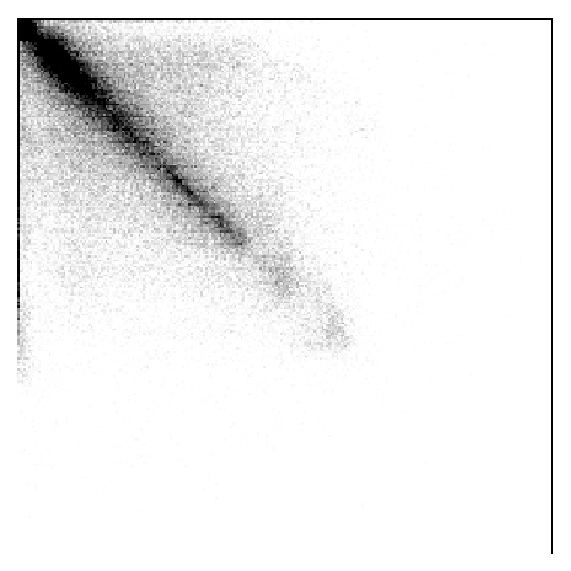
\includegraphics[width=0.2\textwidth]{3_review/figures/processing/registration/histogram/jointhistomisal.eps}}
  \hspace*{\fill}
  \caption[Difference observed in joint histogram between aligned and
  misaligned images.]{Difference observed in joint histogram between aligned
    and misaligned images. The joint measure will be more concentrated of the
    histogram in the case that the images are aligned and more randomly
    distributed in the case that both images are more misaligned.}
  \label{fig:jointhisto}
\end{figure}

In this regard, \ac{mi} was introduced as a similarity measure in registration
framework in the late 1990's by \citeauthor{Pluim2003}~\cite{Pluim2003}.
The \ac{mi} measure finds its foundation in the assumption that a homogeneous
region in the first modality image should also appear as a homogeneous region
in the second modality, even if their \acp{si} are not identical.
Thus, those regions share information and the registration task is achieved by
maximizing this common information.
Hence, \Ac{mi} of two images $A$ and $B$ is defined as:

\begin{equation}
  MI(A;B) = S(A) + S(B) - S(A,B) \ ,
  \label{eq:midef}
\end{equation}

\noindent where $S(A)$, $S(B)$, and $S(A,B)$ are the marginal entropies of $A$
and $B$ and the joint entropy, respectively.
Therefore, maximizing the \ac{mi} is the equivalent of minimizing the joint
entropy.
The joint entropy measure is related to the degree of uncertainty or dispersion
of the data in the joint histogram of the images $A$ and $B$.
As shown in \acs{fig}\,\ref{fig:jointhisto}, the data in the joint histogram
are concentrated in the case of aligned images (see
\acs{fig}\,\ref{subfig:histoalgn}) while it is more randomly distributed in the
case of misaligned images (see \acs{fig}\,\ref{subfig:histomisalgn}).
The entropy is computed based on an estimation of the \ac{pdf} of the images
and thus histogram or Parzen window methods are a common way to estimate these
\acp{pdf}.

A generalized form of \ac{mi}, \ac{cmi}, has been proposed by
\citeauthor{Chappelow2011}~\cite{Chappelow2011}.
\ac{cmi} encompasses interdependent information such as texture and gradient
information into the metric.
Hence, for both of images $A$ and $B$, the image ensembles $\epsilon^{A}_n$ and
$\epsilon^{B}_m$ are generated and composed of $n$ and $m$ images based on the
texture and gradient.
Then, the \ac{cmi} is formulated such as:

\begin{equation}
  CMI(\epsilon^{A}_n;\epsilon^{B}_m) = S(\epsilon^{A}_n) + S(\epsilon^{B}_m) -
  S(\epsilon^{A}_n,\epsilon^{B}_m) \ .
  \label{eq:cmidef}
\end{equation}

From \acs{eq}\,\eqref{eq:cmidef}, note that \ac{cmi} is estimated from
high-dimensional data and as a consequence the histogram-based methods to
estimate the \acp{pdf} are not suitable anymore~\cite{Chappelow2011}.
However, other alternative approaches are used such as the one employed
in~\cite{Staring2009} to compute the $\alpha$-\ac{mi}~\cite{Hero2002}.

\item[] \textbf{Optimization methods}
Registration is usually regarded as an optimization problem where the
parameters of the geometric transformation model have to be inferred by
minimizing/maximizing the similarity measure.
Iterative optimization methods are commonly used, where the most common methods
used are the L-BFGS-B quasi-Newton method~\cite{Byrd1995} and the gradient
descent~\cite{Viola1997}.
During our review, we noticed that authors do not usually linger over optimizer
choice.

\item[] \textbf{Interpolation}
The registration procedure involves transforming an image and pixels mapped to
non-integer points must be approximated using interpolation methods.
As for the optimization methods, we notice that little attention has been paid
on the choice of those interpolations methods.
However, commonly used methods are bi-linear, nearest-neighbour, bi-cubic,
spline, and inverse-distance weighting method~\cite{Mitra2012}.

\item[] \textbf{Registration methods used in \ac{cad} systems}
\acs{tab}~\ref{tab:regtab} summarizes the framework used to register \ac{mpmri}
images in \ac{cad} for \ac{cap}.

\begin{table}
  \centering
  \caption[Classification of the different registration methods used in the
  \acs*{cad} systems reviewed.]{Classification of the different registration
    methods used in the \acs*{cad} systems reviewed. Acronyms: mean squared
    error (MSE), mutual information (MI), combined mutual information (CMI),
    gradient descent (GD), limited-memory Broyden-Fletcher-Goldfarb-Shannon box
    constraints (L-BFGS-B).}
  \scriptsize
  \begin{threeparttable}
    \begin{tabular}{l l c c c c c c c c}\hline
      \toprule
      \textbf{Study} & \textbf{Modality} & \multirow{2}{*}{\textbf{Type}} &
                                                                            \multicolumn{2}{c}{\textbf{Geometric
                                                                            model}}
      & \multicolumn{3}{c}{\textbf{Similarity measure}} &
                                                          \multicolumn{2}{c}{\textbf{Optimizer}}
      \\
      \cmidrule(lr){4-5} \cmidrule(lr){6-8} \cmidrule(lr){9-10}
      \textbf{index} & \textbf{registered} & & Affine & Elastic & \acs{mse} &
                                                                              \acs{mi}
                                           & \acs{cmi} & GD & L-BFGS-B \\
      \midrule
      \cite{Ampeliotis2007,Ampeliotis2008} & \ac{t2w} - \ac{dce} & 2D & \cmark
      & $-$ & \cmark & $-$ & $-$ & $-$ & $-$ \\
      \cite{Giannini2013,giannini2015fully} & \ac{t2w} - \ac{dw} & 2D & \cmark
      & \cmark & $-$ & $-$ & $-$ & $-$ & $-$  \\
      \cite{Giannini2013,giannini2015fully} & \ac{t2w} - \ac{dce} & 2D & \cmark
      & \cmark & $-$ & \cmark & $-$ & \cmark & $-$ \\
      \cite{Viswanath2008a,Viswanath2009} & \ac{t2w} - \ac{dce} & 2D & \cmark &
                                                                                $-$
                                                        & $-$ & \cmark & $-$ &
                                                                               $-$ & $-$ \\
      \cite{Viswanath2011} & \ac{t2w} - \ac{dce} - \ac{dw} & 3D & \cmark & $-$
                                                        & $-$ & $-$ & \cmark &
                                                                               \cmark
                                                      & $-$  \\
      \cite{Vos2008} & \ac{t2w} - \ac{dce} & 3D & \cmark & $-$ & $-$ & \cmark &
                                                                                $-$
                                             & $-$ & $-$ \\
      \cite{Vos2010} & \ac{t2w} - \ac{dce} & 3D & \cmark & \cmark & $-$ &
                                                                          \cmark
                                           & $-$ & $-$ & \cmark \\
      \cite{Lemaitre2016thesis} & \ac{t2w} - \ac{dce} - \ac{dw} & 3D & \cmark & \cmark
                                                        & \cmark & \cmark & $-$ &
                                                                               \cmark
                                                      & $-$  \\
      \bottomrule
    \end{tabular}
    \begin{tablenotes}
      \footnotesize
    \item Notes:
    \item {$-$}: not used or not mentioned.
    \item {\cmark}: used or implemented.
    \end{tablenotes}
  \end{threeparttable}
  \label{tab:regtab}
\end{table}

\citeauthor{Ampeliotis2008} in~\cite{Ampeliotis2007,Ampeliotis2008} did not use
the framework as presented in \acs{fig}\,\ref{fig:frareg} to register 2D
\ac{t2w}-\ac{mri} and \ac{dce}-\ac{mri} images.
By using image symmetries and the \ac{mse} metric, they found the parameters of
an affine transformation but without using a common objective function.
The scale factor, the rotation, and the translation are independently and
sequentially estimated.

\citeauthor{Giannini2013} used also a in-house registration method for 2D
\ac{t2w}-\ac{mri} and \ac{dw}-\ac{mri} images using an affine
model~\cite{Giannini2013,giannini2015fully}.
The bladder is first segmented in both modalities in order to obtain its
contours which are then used as a metric function (i.e. distance between
contours) for registration.

\citeauthor{Giannini2013} and also \citeauthor{Vos2010} used a framework based
on finding an affine transformation to register the \ac{t2w}-\ac{mri} and
\ac{dce}-\ac{mri} images using
\ac{mi}~\cite{Rueckert1999,Giannini2013,Vos2010}.
Then, an elastic registration using B-spline takes place using the affine
parameters to initialize the geometric model with the same similarity measure.
However, the two approaches differ regarding the choice of the optimizer since
a gradient descent is used in~\cite{Giannini2013} and a quasi-Newton method
in~\cite{Vos2010}.
Moreover, \citeauthor{Giannini2013} applied a 2D registration whereas
\citeauthor{Vos2010} registered 3D volumes.

\citeauthor{Viswanath2008a} as well as \citeauthor{Vos2008} registered
\ac{t2w}-\ac{mri} and \ac{dce}-\ac{mri} images using an affine registration and
a \ac{mi} metric~\cite{Viswanath2008a,Viswanath2009,Vos2008}.
However, the choice of the optimizer has not been specified.
Furthermore, \citeauthor{Viswanath2008a} focused on 2D
registration~\cite{Viswanath2008a,Viswanath2009} while \citeauthor{Vos2008}
performed 3D registration~\cite{Vos2008}.

Finally, \citeauthor{Viswanath2011} performed a 3D registration with the three
modalities, \ac{t2w}-\ac{mri}, \ac{dce}-\ac{mri}, and \ac{dw}-\ac{mri}, using
an affine transformation model combined with the \ac{cmi} similarity
measure~\cite{Viswanath2011}.
Moreover, in this latter work, the authors employed a gradient descent
approach~\cite{Chappelow2011} to solve this problem but suggested that the
Nelder-Mead simplex and the quasi-Newton methods are other possible solutions.

\citeauthor{Lemaitre2016thesis} registered \ac{t2w}-\ac{mri},
\ac{dce}-\ac{mri}, and \ac{dw}-\ac{mri} images~\cite{Lemaitre2016thesis}.
The intra-patient motions occurring during \ac{dce}-\ac{mri} is corrected by
rigidly registering all series to the first serie using \ac{mi} and a gradient
descent optimizer.
Once the intra-patient motions are corrected, \ac{t2w}-\ac{mri} and the
\ac{dce}-\ac{mri} are co-registered.
For that matter, the prostate has been segmented in both modalities ---
\ac{t2w}-\ac{mri} and \ac{dce}-\ac{mri} --- to create two binary masks.
Therefore, these 3D binary masks are directly registered using the \ac{mse}
metric and a gradient descent with an elastic registration based on B-splines.
The \ac{t2w}-\ac{mri} and \ac{adc} map acquisitions are registered using the
same approach as for the registration of the \ac{t2w}-\ac{mri} and the
\ac{dce}-\ac{mri} modalities.

\end{enumerate}


%\subsection{Image classification framework}\label{sec:chp3:img-clas}

\subsection{\acs*{cade}: \acsp*{roi} detection/selection} \label{subsec:chp3:img-clas:roiSel}

\begin{table}
  \caption{Overview of the \acs*{cade} strategies employed in \acs*{cad} systems.}
  \centering
  \begin{tabularx}{\textwidth}{l >{\raggedleft\arraybackslash}X}
    \toprule
    \textbf{\ac{cade}: \acp{roi} selection strategy} & \textbf{References} \\
    \midrule
    All voxels-based approach &
    \cite{Artan2009,Artan2010,Giannini2013,Kelm2007,Liu2009,Lopes2011,Matulewicz2013,Mazzetti2011,Ozer2009,Ozer2010,Parfait2012,Sung2011,Tiwari2007,Tiwari2008,Tiwari2009,Tiwari2009a,Tiwari2010,Tiwari2012,Tiwari2013,Viswanath2008,Viswanath2008a,Viswanath2009,Viswanath2011,Viswanath2012,trigui2016classification,trigui2017automatic,lehaire2014computer,khalvati2015automated,rampun2015classifying,rampun2015computer,rampun2016computer,rampun2016computerb,rampun2016quantitative,Lemaitre2016thesis} \\
    Lesions candidate detection & \cite{Litjens2011,Litjens2012,Litjens2014,Vos2012,cameron2014multiparametric,cameron2016maps} \\
    \bottomrule
  \end{tabularx}
  \label{tab:cade}
\end{table}

As discussed in the introduction and shown in \acs{fig}\,\ref{fig:wkfcad}, the
image classification framework is often composed of a \ac{cade} and a
\ac{cadx}.
In this section, we focus on studies which embed a \ac{cade} in their framework.
Two approaches are considered to define a \ac{cade}: (i) voxel-based
delineation and (ii) lesion segmentation.
These methods are summarized in \acs{tab}~\ref{tab:cade}.
The first strategy is in fact linked to the nature of the classification
framework and concerns the majority of the studies
reviewed~\cite{Artan2009,Artan2010,Giannini2013,Kelm2007,Liu2009,Lopes2011,Matulewicz2013,Mazzetti2011,Ozer2009,Ozer2010,Parfait2012,Sung2011,Tiwari2007,Tiwari2008,Tiwari2009,Tiwari2009a,Tiwari2010,Tiwari2012,Tiwari2013,Viswanath2008,Viswanath2008a,Viswanath2009,Viswanath2011,Viswanath2012,trigui2016classification,trigui2017automatic,lehaire2014computer,khalvati2015automated,rampun2015classifying,rampun2015computer,rampun2016computer,rampun2016computerb,rampun2016quantitative,Lemaitre2016thesis}.
Each voxel is a possible candidate and will be classified as cancer or healthy.
The second group of methods is composed of method implementing a lesion
segmentation algorithm to delineate potential candidates to further obtain a
diagnosis through the \ac{cadx}.
This approach is borrowed from other application areas such as breast cancer.
These methods are in fact very similar to the classification framework used in
\ac{cadx} later.

Regarding lesion candidate detection, \citeauthor{Vos2012} highlighted lesion
candidates by detecting blobs in the \ac{adc} map~\cite{Vos2012}.
These candidates are filtered using some \textit{a priori} criteria such as
\ac{si} or diameter.
As mentioned in \acs{sec}\,\ref{subsec:chp2:imaging:mrsi} and
\acs{tab}~\ref{tab:modmri}, low \ac{si} in \ac{adc} map can be linked to
potential \ac{cap}.
Hence, blob detectors are suitable to highlight these regions.
Blobs are detected in a multi-resolution scheme, by computing the three main
eigenvalues $\{ \lambda_{\sigma,1},\lambda_{\sigma,2},\lambda_{\sigma,3} \}$ of
the Hessian matrix, for each voxel location of the \ac{adc} map at a specific
scale $\sigma$~\cite{Li2003}.
The probability $p$ of a voxel $\mathbf{x}$ being a part of a blob at the scale
$\sigma$ is given by:

\begin{equation}
  P(\mathbf{x},\sigma) = \begin{cases}
    \frac{\| \lambda_{\sigma,3}(\mathbf{x}) \|^{2}}{\| \lambda_{\sigma,1}
      (\mathbf{x}) \|} \ , & \text{if } \lambda_{\sigma,k}(\mathbf{x}) > 0
    \text{ with } k = \{1,2,3\} \  , \\
    0 \ , & \text{otherwise} \ .
  \end{cases}
  \label{eq:blobdet}
\end{equation}

\noindent The fusion of the different scales is computed as:

\begin{equation}
  L(\mathbf{x}) = \max P(\mathbf{x},\sigma) , \forall \sigma \ .
  \label{eq:fusionBlob}
\end{equation}

The candidate blobs detected are then filtered depending on their appearances
--- i.e., maximum of the likelihood of the region, diameter of the lesion ---
and their \ac{si} in \ac{adc} and \ac{t2w}-\ac{mri} images.
The detected regions are then used as inputs for the \ac{cadx}.
\citeauthor{cameron2016maps} used a similar approach by automatically selecting
low \ac{si} connected regions in the \ac{adc} map with a size larger than
\SI{1}{\milli\metre\squared}~\cite{cameron2014multiparametric,cameron2016maps}.

\citeauthor{Litjens2011} used a pattern recognition approach in order to
delineate the \acp{roi}~\cite{Litjens2011}.
A blobness map is computed in the same manner as in~\cite{Vos2010} using the
multi-resolution Hessian blob detector on the \ac{adc} map, \ac{t2w}, and
pharmacokinetic parameters maps (see
\acs{sec}\,\ref{subsec:chp3:img-clas:CADX-fea-dec} for details about those
parameters).
Additionally, the position of the voxel $\mathbf{x}=\{x,y,z\}$ is used as a
feature as well as the Euclidean distance of the voxel to the prostate center.
Hence, each feature vector is composed of 8 features and a \ac{svm} classifier
is trained using a \ac{rbf} kernel (see
\acs{sec}\,\ref{subsec:chp3:img-clas:CADX-clas} for more details).

Subsequently, \citeauthor{Litjens2012} modified this approach by including only
features related to the blob detection on the different maps as well as the
original \acp{si} of the parametric images~\cite{Litjens2012}.
Two new maps are introduced based on texture and a \ac{knn} classifier is used
instead of a \ac{svm} classifier.
The candidate regions are then extracted by performing a local maxima detection
followed by post-processing region-growing and morphological operations.

\subsection{\acs*{cadx}: Feature detection} \label{subsec:chp3:img-clas:CADX-fea-dec}

Discriminative features which help to recognize \ac{cap} from healthy tissue
need to be first detected.
This processing is known in computer vision as feature extraction.
However, feature extraction also refers to the name given in pattern
recognition to some types of dimension reduction methods which are later
presented.
In order to avoid confusion between these two aspects, in this survey, the
procedure ``detecting'' or ``extracting'' features from images and signals is
defined as feature detection.
This section summarizes the different features used in \ac{cad} for \ac{cap}.

\subsubsection{Image-based features}\label{subsubsec:chp3:img-clas:CADX-fea-dec:Img-fea}

This section focuses on image-based features which can be categorized into two
categories: (i) voxel-wise detection and (ii) region-wise detection.

\setenumerate{listparindent=\parindent,itemsep=10px}
\setlist{noitemsep}
\begin{enumerate}[leftmargin=*]

\item[] \textbf{Voxel-wise detection in \acs*{mri}}
This strategy refers to the fact that a feature is extracted at each voxel
location.
As discussed in \acs{chp}\,\ref{chap:2}, \ac{cap} has an influence on the
\ac{si} in \ac{mpmri} images.
Therefore, intensity-based feature is the most commonly used
feature~\cite{Ampeliotis2007,Ampeliotis2008,Vos2008,rampun2016computerb,rampun2015classifying,Giannini2013,Artan2009,Artan2010,Chan2003,Langer2009,Litjens2011,Litjens2012,Litjens2014,Liu2009,Ozer2009,Ozer2010,trigui2016classification,trigui2017automatic,cameron2014multiparametric,cameron2016maps,khalvati2015automated,chung2015prostate,giannini2015fully,Niaf2011,Niaf2012,lehaire2014computer,Lemaitre2016thesis}.
This feature consists in the extraction of the intensity of the \ac{mri}
modality of interest.

Edge-based features have also been used to detect \ac{si} changes but bring
additional information regarding the \ac{si} transition.
Each feature is computed by convolving the original image with an edge operator.
Three operators are commonly used: (i) Prewitt operator~\cite{Prewitt1970},
(ii) Sobel operator~\cite{Sobel1970}, and (iii) Kirsch
operator~\cite{Kirsch1971}.
These operators differ due to the kernel used which attenuates more or less the
noise.
Multiple studies used the resulting magnitude and orientation of the edges
computed in their classification
frameworks~\cite{Niaf2011,Niaf2012,Tiwari2009a,Tiwari2010,Tiwari2013,Viswanath2008,Viswanath2011,rampun2016quantitative,rampun2015computer,rampun2016computer,lehaire2014computer,khalvati2015automated,chung2015prostate,Lemaitre2016thesis}.

\begin{figure}
  \hspace*{\fill}
  \subfloat[$\theta=0^{\circ}$.]{\label{subfig:gab1}
    
\includegraphics[width=0.2\linewidth]{3_review/figures/feature-detection/gabor/gabor_1.eps}}
  \hfill
  \subfloat[$\theta=60^{\circ}$.]{\label{subfig:gab2}
    
\includegraphics[width=0.2\linewidth]{3_review/figures/feature-detection/gabor/gabor_2.eps}}
  \hfill
  \subfloat[$\theta=120^{\circ}$.]{\label{subfig:gab3}
    
\includegraphics[width=0.2\linewidth]{3_review/figures/feature-detection/gabor/gabor_3.eps}}
  \hfill
  \subfloat[$\theta=180^{\circ}$.]{\label{subfig:gab4}
    
\includegraphics[width=0.2\linewidth]{3_review/figures/feature-detection/gabor/gabor_4.eps}}
  \hspace*{\fill}
  \caption[Illustration of 4 different Gabor filters.]{Illustration of 4
    different Gabor filters varying their orientations $\theta$.}
  \label{fig:gabor}
\end{figure}

Gabor filters~\cite{Gabor1946,Daugman1985} offer an alternative to the usual
edge detector, with the possibility to tune the direction and the frequency of
the filter to encode a specific pattern.
A Gabor filter is defined by the modulation of a Gaussian function with a sine
wave which can be further rotated and is formalized as in
\acs{eq}\,\ref{eq:gabor}.
\begin{equation}
  g(x,y;\theta,\psi,\sigma,\gamma) = \exp \left( - \frac{x'^{2}+
      \gamma^{2}y'^{2}}{2 \sigma^{2}} \right) \cos \left( 2 \pi
    \frac{x'}{\lambda} + \psi \right) \ ,
  \label{eq:gabor}
\end{equation}

\noindent with

\begin{eqnarray}
  x' & = & s\left( x \cos \theta + y \sin \theta \right) \ , \nonumber \\
  y' & = & s \left( - x \sin \theta + y \cos \theta \right) \ , \nonumber
\end{eqnarray}

\noindent where $\lambda$ is the wavelength of the sinusoidal factor, $\theta$
represents the orientation of the Gabor filter, $\psi$ is the phase offset,
$\sigma$ is the standard deviation of the Gaussian envelope, $\gamma$ is the
spatial aspect ratio, and $s$ is the scale factor.
In an effort to characterize pattern and texture, a bank of Gabor filters is
usually created with different angles, scale, and frequency --- refer to
\acs{fig}\,\ref{fig:gabor} --- and then convolved with the image.
\citeauthor{Viswanath2012}~\cite{Viswanath2012},
\citeauthor{Tiwari2012}~\cite{Tiwari2012} and more recently
\citeauthor{khalvati2015automated}~\cite{khalvati2015automated} and
\citeauthor{chung2015prostate}~\cite{chung2015prostate} have designed a bank of
Gabor filters to characterized texture and edge information in
\ac{t2w}-\ac{mri} and \ac{dw}-\ac{mri} modalities.

\citeauthor{Lemaitre2016thesis}~\cite{Lemaitre2016thesis} used a 3D Gabor
filters bank.
3D Gabor filters~\cite{wang2005face} are not commonly used and we recall their
formulation in \acs*{eq}\,\eqref{eq:gabor3d}.

\begin{equation}
  g(\mathbf{x};\boldsymbol{\sigma},f,\theta,\phi) = \hat{g}(\mathbf{x};\boldsymbol{\sigma}) \exp(j 2 \pi f \left( x \sin \theta \cos \phi + y \sin \theta \sin \phi + z \cos \theta \right)) \ ,
  \label{eq:gabor3d}
\end{equation}

\noindent where,

\begin{equation}
  \hat{g}(\mathbf{x};\boldsymbol{\sigma}) = \frac{1}{{\left(2 \pi\right)}^{\frac{3}{2}}} \exp \left( -\frac{1}{2} \left( \frac{x^2}{\sigma_x^2} + \frac{y^2}{\sigma_y^2} + \frac{z^2}{\sigma_z^2} \right) \right) \ ,
  \label{eq:gabor3dgaussian}
\end{equation}

\noindent where $\mathbf{x}$ is the position vector $\{x,y,z\}$,
$\boldsymbol{\sigma}$ is the standard deviation vector
$\{\sigma_x,\sigma_y,\sigma_z\}$ of the 3D Gaussian envelope, $f$ is the radial
center frequency of the sine wave, $\theta$ is the elevation angle, and $\phi$
is the azimuth angle.

Additionally, \citeauthor{Lemaitre2016thesis}~\cite{Lemaitre2016thesis}
features based on phase congruency as proposed by\citeauthor{kovesi1999image}
are computed~\cite{kovesi1999image}.
Therefore, from a set of Log-Gabor filter bank, the orientation image, the
local weighted mean phase angle, and the phase angle are estimated at each
voxel.

Texture-based features provide other characteristics discerning \ac{cap} from
healthy tissue.
The most common texture analysis for image classification is based on the
\ac{glcm} with their related statistics which have been proposed by
\citeauthor{Haralick1973} in~\cite{Haralick1973}.
In a neighborhood around a central voxel, a \ac{glcm} is build considering each
voxel pair defined by a specific distance and angle.
Then, using the \ac{glcm}, a set of statistical features is computed as defined
in \acs{tab}~\ref{tab:glcm} and assigned to the location of the central voxel.
Therefore, $N$ --- up to 14 --- statistical maps are derived from the \ac{glcm}
analysis, one per statistics presented in \acs{tab}~\ref{tab:glcm}.
\ac{glcm} is commonly used in \ac{cad} systems, on the different \ac{mri}
modalities, namely \ac{t2w}-\ac{mri}, \ac{dce}-\ac{mri}, or
\ac{dw}-\ac{mri}~\cite{Antic2013,Niaf2011,Niaf2012,Tiwari2009a,Tiwari2010,Tiwari2013,Viswanath2008,Viswanath2009,Viswanath2011,Viswanath2012,trigui2016classification,rampun2015computer,rampun2016computer,rampun2016quantitative,cameron2014multiparametric,cameron2016maps,khalvati2015automated,chung2015prostate,lehaire2014computer,Lemaitre2016thesis}.
However, the statistics extracted from the \ac{glcm} across studies vary.
Along the same line, \citeauthor{rampun2016computer} extracted from
\ac{t2w}-\ac{mri}~\cite{rampun2016computer,rampun2015computer} Tamura
features~\cite{tamura1978textural} composed of three features to characterize
texture: (i) coarseness, (ii) contrast, and (iii) directionality.

\begin{table}
  \caption[The 14 statistical features used in conjunction with \acs*{glcm}
  analysis.]{The 14 statistical features for texture analysis commonly computed
    from the \acs*{glcm} $p$ as presented by~\cite{Haralick1973}.}
  \renewcommand{\arraystretch}{1.5}
  \centering
  \begin{tabular}{ll}
    \toprule
    \textbf{Statistical features} & \textbf{Formula} \\
    \midrule
    Angular second moment & $\sum_i \sum_j p(i,j)^2 $  \\
    Contrast & $\sum_{n=0}^{N_g - 1} n^2 \left[ \sum_{i=1}^{N_g - 1}
               \sum_{j=1}^{N_g - 1} p(i,j) \right] \ , | i-j |=n  $ \\
    Correlation & $\frac{\sum_i \sum_j (ij) p(i,j) - \mu_x \mu_y}{\sigma_x \sigma_y}  $ \\
    Variance & $\sum_i \sum_j (i - \mu)^2 p(i,j)  $ \\
    Inverse difference moment & $\sum_i \sum_j \frac{1}{1+(i - \mu)^2} p(i,j)  $ \\
    Sum average & $\sum_{i=2}^{2N_g} i p_{x+y}(i)  $ \\
    Sum variance & $\sum_{i=2}^{2N_g} (i-f_s)^2 p_{x+y}(i)  $ \\
    Sum entropy & $ - \sum_{i=2}^{2N_g} p_{x+y}(i) \log p_{x+y}(i)  $ \\
    Entropy & $ - \sum_i \sum_j p(i,j) \log p(i,j) $ \\
    Difference variance & $\sum_{i=0}^{N_g-1} i^2 p_{x-y}(i)  $ \\
    Difference entropy & $ - \sum_{i=0}^{N_g-1} p_{x-y}(i) \log p_{x-y}(i)  $ \\
    Info. measure of corr. 1 & $\frac{S(X;Y)-S_1(X;Y)}{\max(S(X),S(Y))}  $ \\
    Info. measure of corr. 2 & $\sqrt{\left( 1 - \exp \left[ -2( H_2(X;Y) - H(X;Y) ) \right] \right)}  $ \\
    Max. corr. coeff. & $ \sqrt{\lambda_2} \ , \text{of } Q(i,j) = \sum_k \frac{p(i,k)p(j,k)}{p_x(i)p_y(k)}  $ \\
    \bottomrule
  \end{tabular}
  \label{tab:glcm}
\end{table}

\citeauthor{Lopes2011} used fractal analysis  and more precisely a local
estimation of the fractal dimension~\cite{Benassi1998}, to describe the texture
roughness at a specific location.
The fractal dimension is estimated through a wavelet-based method in
multi-resolution analysis.
They showed that cancerous tissues have a higher fractal dimension than healthy
tissue.

\citeauthor{Chan2003} described texture using the frequency signature via the
\acf{dct}\cite{Ahmed1974} defining a neighbourhood of
\SI[product-units=repeat]{7x7}{\px} for modalities used, namely
\ac{t2w}-\ac{mri} and \ac{dw}-\ac{mri}.
The \ac{dct} allows to decompose a portion of an image into a coefficient
space, where few of these coefficients encode the significant information.
The \ac{dct} coefficients are computed such as:

\begin{equation}
  C_{k_1,k_2} = \sum_{m=0}^{M-1} \sum_{n=0}^{N-1} p_{m,n} \cos \left[
    \frac{\pi}{M} \left( m + \frac{1}{2} \right) k_1 \right] \cos \left[
    \frac{\pi}{N} \left( n + \frac{1}{2} \right) k_2 \right] \ ,
\end{equation}

\noindent where $C_{k_1,k_2}$ is the \ac{dct} coefficient at the position
$k_1,k_2$, $M$ and $N$ are the dimension of the neighbourhood and $p_{m,n}$ is
the pixel \ac{si} at the position $\{m,n\}$.

\citeauthor{Lemaitre2016thesis}~\cite{Lemaitre2016thesis} incorporated those
features in their \ac{cad} system.

Regarding other features, \citeauthor{Viswanath2012} projected
\ac{t2w}-\ac{mri} images into the wavelet space, using the Haar wavelet, and
used the resulting coefficients as features~\cite{Viswanath2012}.
\citeauthor{Litjens2011} computed the texture map based on \ac{t2w}-\ac{mri}
images using a Gaussian filter bank~\cite{Litjens2011}.
Likewise, \citeauthor{rampun2016computer} employed a rotation invariant filter
bank proposed in~\cite{leung2001representing}.
The bank is composed of 48 filters including Gaussian filters, first and second
derivatives of Gaussian filters as well as Laplacian of Gaussian.

\item[] \textbf{Region-wise detection in \acs*{mri}}
Unlike the previous section, another strategy is to study a region instead of
each pixel independently.
Usually, the feature maps are computed using the method presented in
voxel-based approach followed by a step in which features are computed in some
specific delineated regions to characterize them.

The most common feature type is based on statistics and more specifically the
statistic-moments such as mean, standard deviation, kurtosis, and
skewness~\cite{Ampeliotis2007,Ampeliotis2008,Tiwari2009a,Tiwari2010,Tiwari2013,Viswanath2008,Viswanath2009,Viswanath2012,rampun2016quantitative,rampun2015computer,rampun2016computer,Antic2013,Viswanath2011,Peng2013,cameron2014multiparametric,cameron2016maps,khalvati2015automated,chung2015prostate,Litjens2011,Litjens2012,Litjens2014,Niaf2011,Niaf2012,lehaire2014computer}.
Additionally, some studies extract additional statistical landmarks based on
percentiles~\cite{Vos2008a,Antic2013,Peng2013,Vos2010,Litjens2011,Litjens2012,Litjens2014,Niaf2011,Niaf2012,Vos2012,lehaire2014computer}
The percentiles to use are manually determined by observing the \ac{pdf} of the
features and checking which values allow the best to differentiate malignant
from healthy tissue.

Further statistics are computed through the use of histogram-based features.
\citeauthor{Liu2013} introduced 4 different types of histogram-based features
to characterize hand-delineated lesions~\cite{Liu2013}.
The first type corresponds to the histogram of the \ac{si} of the image.
The second type is the \ac{hog}~\cite{Dalal2005} which encodes the local shape
of the object of interest by using the distribution of the gradient
directions.
This descriptor is extracted mainly in three steps.
First, the gradient image and its corresponding magnitude and direction are
computed.
Then, the \ac{roi} is divided into cells and an oriented-based histogram is
generated for each cell.
At each pixel location, the orientation of the gradient votes for a bin of the
histogram and this vote is weighted by the magnitude of the same gradient.
Finally, the cells are grouped into blocks and each block is normalized.
The third histogram-based type used in~\cite{Liu2013} is the shape context
introduced in~\cite{Belongie2002}.
The shape context is also a way to describe the shape of an object of interest.
First, a set of points defining edges have to be detected and for each point of
each edge, a log-polar-based histogram is computed using the relative points
distribution.
The last set of histogram-based feature extracted is based on the framework
described in~\cite{Zhao2012} which is using the Fourier transform of the
histogram created via \acf{lbp}~\cite{Ojala1996}.
\Ac{lbp} is generated by comparing the value of the central pixel with its
neighbours, defined through a radius and the number of connected neighbours.
Then, in the \ac{roi}, the histogram of the \ac{lbp} distribution is computed.
The \acf{dft} of the \ac{lbp} histogram is used to make the feature invariant
to rotation.

Another subset of features are anatomical-based features and have been used
in~\cite{Litjens2012,Litjens2014,Matulewicz2013,cameron2014multiparametric,cameron2016maps}.
\citeauthor{Litjens2012} computed the volume, compactness, and sphericity
related to the given region~\cite{Litjens2012, Litjens2014}.
Additionally, \citeauthor{Litjens2014} also introduced a feature based on
symmetry in which they compute the mean of a candidate lesion as well as its
mirrored counter-part and compute the quotient as feature~\cite{Litjens2014}.
\citeauthor{Lemaitre2016thesis}~\cite{Lemaitre2016thesis} incorporated those
features in their \ac{cad} system.
\citeauthor{Matulewicz2013} introduced 4 features corresponding to the
percentage of tissue belonging to the regions \ac{pz}, \ac{cg}, periurethral
region, or outside the prostate region for the considered
\ac{roi}~\cite{Matulewicz2013}.
Finally, \citeauthor{cameron2016maps} defined 4 features based on morphology
and asymmetry:
(i) the difference of morphological closing and opening of the \ac{roi}, (ii)
the difference of the initial perimeter and the one after removing the
high-frequency components, (iii) the difference between the initial \ac{roi}
and the one after removing the high-frequency components, and (iv) the
asymmetry by computing the difference of the two areas splitting the \ac{roi}
by its major axes~\cite{cameron2014multiparametric,cameron2016maps}.

The last group of region-based feature is based on fractal analysis.
This group of features is based on estimating the fractal dimension which is a
statistical index representing the complexity of the analyzed texture.
\citeauthor{Lv2009} proposed two features based on fractal dimension: (i)
texture fractal dimension and (ii) histogram fractal dimension~\cite{Lv2009}.
The first feature is based on estimating the fractal dimension on the \ac{si}
of each image and thus this feature is a statistical characteristic of the
image roughness.
The second fractal dimension is estimated using the \ac{pdf} of each image and
characterizes the complexity of the \ac{pdf}.
\citeauthor{Lopes2011} proposed a 3D version to estimate the fractal dimension
of a volume using a wavelet decomposition~\cite{Lopes2011}.

\end{enumerate}

\subsubsection{\acs*{dce}-based features}\label{subsubsec:chp3:img-clas:CADX-fea-dec:DCE-fea}

\ac{dce}-\ac{mri} is more commonly based on a \ac{si} analysis over time as
presented in \acs{sec}\,\ref{subsec:chp2:imaging:dce}.
In this section, the specific features extracted for \ac{dce}-\ac{mri} analysis
are presented.

\begin{table}
  \caption{Parameters used as features for a \acs*{dce} semi-quantitative analysis in \acs*{cad} systems.}
  \centering
  \begin{tabularx}{\textwidth}{l X}
    \toprule
    \textbf{Semi-quantitative features} & \textbf{Explanations} \\
    \midrule
    \textbf{Amplitude features:} & \\ \\ [-1.5ex]
    \quad $S_0$ & Amplitude at the onset of the enhancement \\
    \quad $S_{\max}$ & Amplitude corresponding to $95\%$ of the maximum amplitude \\
    \quad $S_{p}$ & Amplitude corresponding to the maximum amplitude \\
    \quad $S_f$ & Amplitude at the final time point \\ \\ [-1.5ex]
    \textbf{Time features:} & \\ \\ [-1.5ex]
    \quad $t_0$ & Time at the onset of the enhancement \\
    \quad $t_{\max}$ & Time corresponding to $95\%$ of the maximum amplitude \\
    \quad $t_{p}$ & Time corresponding to the maximum amplitude \\
    \quad $t_{f}$ & Final time \\
    \quad $t_{tp}$ & Time to peak which is the time from $t_0$ to $t_p$ \\ \\ [-1.5ex]
    \textbf{Derivatives and integral features:} & \\ \\ [-1.5ex]
    \quad $WI$ & Wash-in rate corresponding to the signal slope from $t_0$ to $t_m$ or $t_p$ \\
    \quad $WO$ & Wash-out rate corresponding to the signal slope from $t_m$ or $t_p$ to $t_p$ \\
    \quad $IAUC$ & Initial area under the curve which is the area between $t_0$ to $t_{f}$ \\
    \bottomrule
  \end{tabularx}
  \label{tab:semiqua}
\end{table}

\setenumerate{listparindent=\parindent,itemsep=10px}
\setlist{noitemsep}
\begin{enumerate}[leftmargin=*]

\item[] \textbf{Whole-spectra approach}
Some studies are using the whole \ac{dce} time series as feature
vector~\cite{Ampeliotis2007,Ampeliotis2008,Tiwari2012,Viswanath2008a,Viswanath2008,Lemaitre2016thesis}.
In some cases, the high-dimensional feature space is reduced using dimension
reduction methods as it will be presented in the
\acs{sec}\,\ref{subsec:chp3:img-clas:CADX-fea-ext}.

\begin{figure}
  \centering
  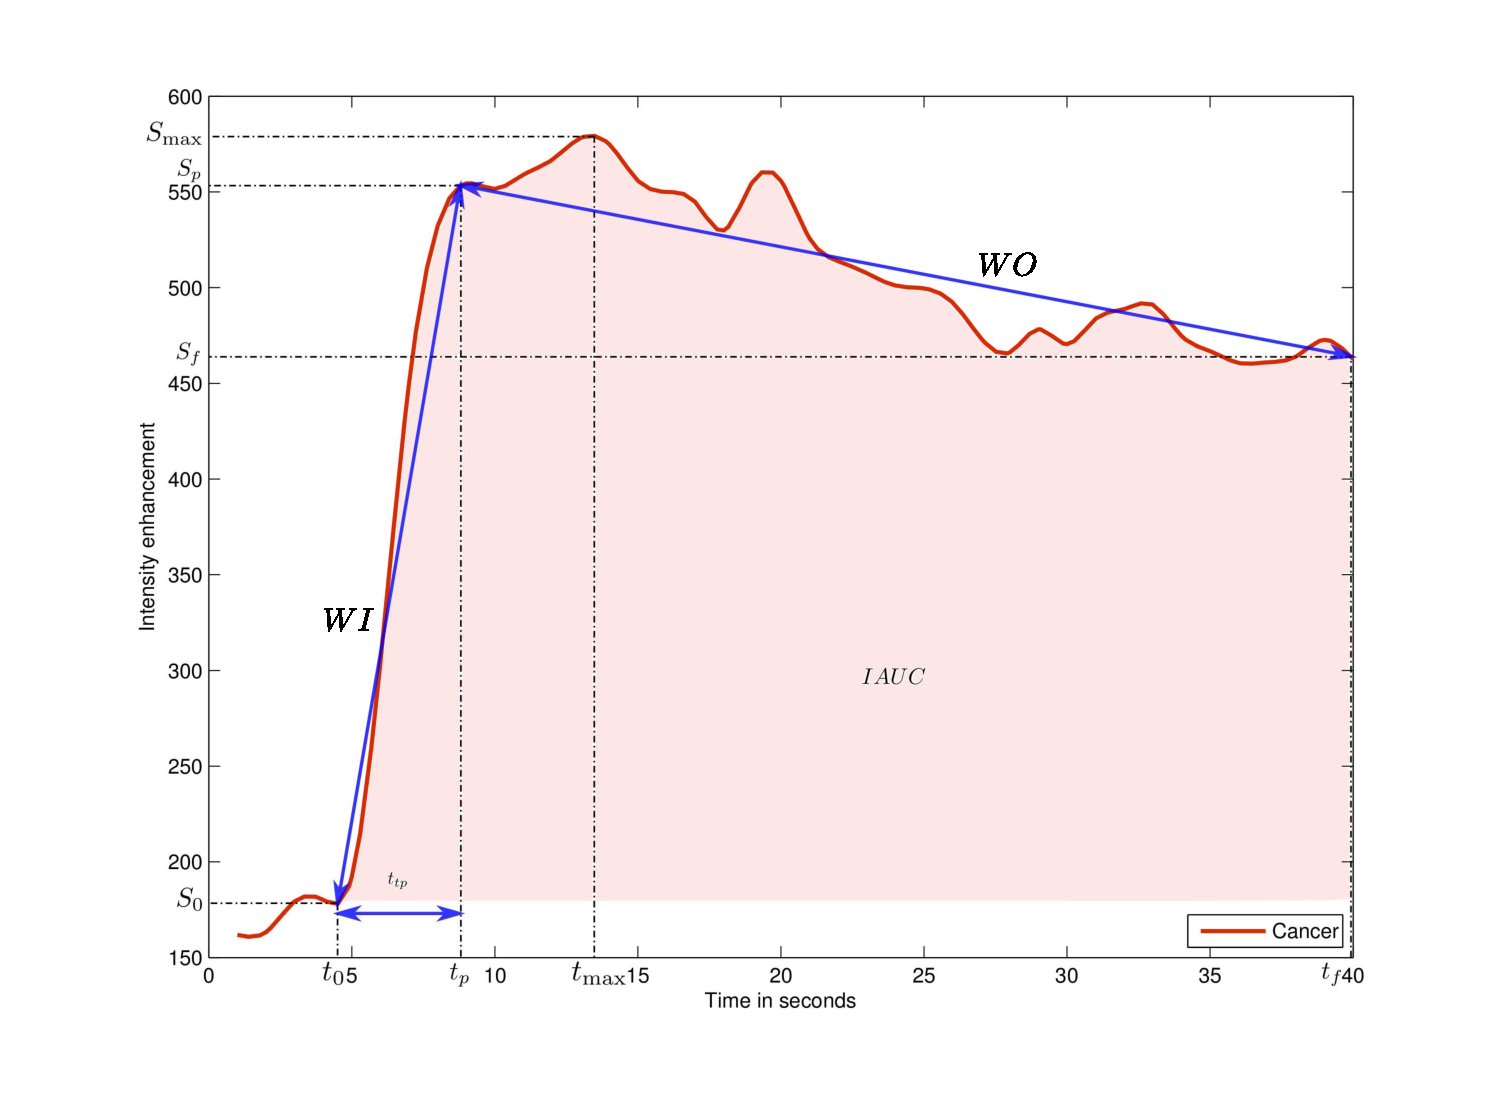
\includegraphics[width=.8\linewidth]{3_review/figures/feature-detection/dce/dce_cancer_parameters.eps}
  \caption[Semi-quantitative features used for
  \acs*{dce}-\acs*{mri}.]{Graphical representation of the different
    semi-quantitative features used for \acs*{dce}-\acs*{mri} analysis.}
  \label{fig:dceparam}
\end{figure}

\item[] \textbf{Semi-quantitative approach}
Semi-quantitative approaches are based on mathematically modelling the \ac{dce}
time series.
The parameters modelling the signal are commonly used, mainly due to the
simplicity of their
computation~\cite{Puech2009,Mazzetti2011,Niaf2011,Niaf2012,Sung2011,trigui2016classification,trigui2017automatic,lehaire2014computer,samarasinghe2016semi,giannini2015fully,Lemaitre2016thesis}.
Parameters included in semi-quantitative analysis are summarized in
\acs{tab}~\ref{tab:semiqua} and also graphically depicted in
\acs{fig}\,\ref{fig:dceparam}.
A set of time features corresponding to specific amplitude level (start,
maximum, and end) are extracted.
Then, derivative and integral features are also considered as discriminative
and are commonly computed.

\item[] \textbf{Quantitative approach}
As presented in \acs{chp}\,\ref{chap:2}, quantitative approaches correspond to
mathematical-pharmacokinetic models based on physiological exchanges.
Four different models have been used in \ac{cad} for \ac{cap} systems.
The most common model reviewed is the \textit{Brix
  model}~\cite{Artan2009,Artan2010,Sung2011,Liu2009,Ozer2009,Ozer2010,Lemaitre2016thesis}.
This model is formalized such as:

\begin{equation}
  \frac{S(t)}{S(0)} = 1 + A k_{ep} \left( \frac{\exp( -k_{ep} t ) - \exp(
      -k_{el} t )}{k_{el} - k_{ep}} \right) \ ,
  \label{eq:brixmod}
\end{equation}

\noindent where $S(\cdot)$ is the \ac{dce} signal, $A$ is the parameter
simulating the tissue properties, $k_{el}$ is the parameter related to the
first-order elimination from the plasma compartment, and $k_{ep}$ is the
parameter of the transvascular permeability.
The parameters $k_{ep}$, $k_{el}$, and $A$ are computed from the \ac{mri} data
and used as features.

Another model is Tofts model~\cite{Tofts1997} which has been used
in~\cite{Langer2009,Giannini2013,Niaf2011,Niaf2012,Mazzetti2011,lehaire2014computer,giannini2015fully,Lemaitre2016thesis}.
In this model, the \ac{dce} signal relative to the concentration is presented
as:
\begin{equation}
  C_t(t) = v_p C_p(t) + K_{trans} \int_{0}^{t} C_p(\tau) \exp( -k_{ep}(t-\tau)
  ) \ d\tau \ ,
  \label{eq:tofts}
\end{equation}

\noindent where $C_t(\cdot)$ is the concentration of the medium, $C_p(\cdot)$
is the \ac{aif} which has to be estimated independently, $K_{trans}$ is the
parameter related to the diffuse transport of media across the capillary
endothelium, $k_{ep}$ is the parameter related to the exchanges back into the
vascular space, and $v_e$ is the extravascular-extracellular space fraction
defined such that $v_e = 1 - v_p$.
In this model, parameters $K_{trans}$, $k_{ep}$, and $v_e$ are computed and
used as features.

\citeauthor{Mazzetti2011}, \citeauthor{giannini2015fully}, and
\citeauthor{Lemaitre2016thesis} used the Weibull
function~\cite{Mazzetti2011,Giannini2013,giannini2015fully,Lemaitre2016thesis}
which is formalized as:

\begin{equation}
  S(t) = A t \exp( -t^{B} ) \ ,
  \label{eq:weibull}
\end{equation}

\noindent where $A$ and $B$ are the two parameters which have to be inferred.

They also used another empirical model which is based on the West-like function
and named the \ac{pun}~\cite{Castorina2006}, formalized as:

\begin{equation}
  S(t) = \exp \left[ r t + \frac{1}{\beta} a_0 - r \left( \exp( \beta t ) - 1
    \right) \right] \ ,
  \label{eq:pun}
\end{equation}
\noindent where the parameters $\beta$, $a_0$ and $r$ are inferred.
For all these models, the parameters are inferred using an optimization curve
fitting approach.

\end{enumerate}

\subsubsection{\acs*{mrsi}-based features}\label{subsubsec:chp3:img-clas:CADX-fea-dec:MRSI-fea}

\setenumerate{listparindent=\parindent,itemsep=10px}
\setlist{noitemsep}
\begin{enumerate}[leftmargin=*]

\item[] \textbf{Whole spectra approach in \acs*{mrsi}}
As in the case of \ac{dce} analysis, one common approach is to incorporate the
whole \ac{mrsi} spectra in the feature vector for
classification~\cite{Kelm2007,Parfait2012,Tiwari2007,Tiwari2009,Tiwari2013,Tiwari2009a,Tiwari2010,Viswanath2008a,Matulewicz2013,trigui2016classification,trigui2017automatic,
Lemaitre2016thesis}.
Sometimes post-processing involving dimension reduction methods is performed to
reduce the complexity during the classification as it will be presented in
\acs{sec}\,\ref{subsec:chp3:img-clas:CADX-fea-ext}.

\item[] \textbf{Quantification approach in \acs*{mrsi}}
We can reiterate that in \ac{mrsi} only few biological markers --- i.e.,
choline, creatine, and citrate metabolites --- are known to be useful to
discriminate \ac{cap} and healthy tissue.
Therefore, only the concentrations of these metabolites are considered as a
feature prior to classification.
In order to perform this quantification, 4 different approaches have been used.
\citeauthor{Kelm2007} used the following models~\cite{Kelm2007}:
QUEST~\cite{Ratiney2005}, AMARES~\cite{Vanhamme1997}, and
VARPRO~\cite{Coleman1993}.
They are all time-domain quantification methods varying by the type of
pre-knowledge embedded and the optimization approaches used to solve the
quantification problem.
Unlike the time-domain quantification approaches, \citeauthor{Parfait2012} used
the LcModel approach proposed in~\cite{Provencher1993} which solves the
optimization problem in the frequency domain.
Although \citeauthor{Parfait2012} and \citeauthor{Lemaitre2016thesis} used each metabolite relative concentration
individually~\cite{Parfait2012,Lemaitre2016thesis}, other authors such as \citeauthor{Kelm2007}
proposed to compute relative concentrations as the ratios of metabolites as
shown in \acs{eq}\,\ref{eq:ratio1} and \acs{eq}\,\ref{eq:ratio2}.

\begin{eqnarray}
  R_1 & = & \frac{ [ \text{Cho} ] + [ \text{Cr} ]}{[ \text{Cit} ]} \ . \label{eq:ratio1} \\
  R_2 & = & \frac{[ \text{Cit} ]}{[\text{Cho}]+[\text{Cr}]+[\text{Cit}]} \ , \label{eq:ratio2}
\end{eqnarray}
\noindent where $\text{Cit}$, $\text{Cho}$ and $\text{Cr}$ are the relative
concentration of citrate, choline, and creatine, respectively.

Recently \citeauthor{trigui2017automatic} used an absolute quantification
approach from which water sequences are acquired to compute the absolute
concentration of the
metabolites~\cite{trigui2016classification,trigui2017automatic}.
Absolute quantification using water as reference is based on the fact that the
fully relaxed signal from water or metabolites is proportional to the number of
moles of the molecules in the voxel~\cite{gasparovic2006use}.

\item[] \textbf{Wavelet decomposition approach in \acs*{mrsi}}
\citeauthor{Tiwari2012} performed a wavelet packet
decomposition~\cite{Coifman1992} of the spectra using the Haar wavelet basis
function and use its coefficients as features.

\end{enumerate}

The feature detection methods used in \ac{cad} are summarized in
\acs{tab}~\ref{tab:feat}.

% \input{3_review/Table-CADX-feature-detection}
\begin{landscape}
  \input{3_review/table_feature_detection}
\end{landscape}

\subsection{Feature balancing}\label{subsec:chp6:method:fea-bal}
Data imbalanced is a recurrent issue in classification, notably in medical
data.
The problem of imbalanced dataset lies in the fact that one of the class has a
smallest number of data --- i.e., in medical data, the class corresponding to
patients with a disease --- compared with the other classes.
Therefore, solving the problem of imbalanced is equivalent to under- or
over-sampling part of the dataset to obtain equal number of samples in the
different classes.
Recently, \citeauthor{Lemaitre2016thesis} used balancing methods during the
learning stage to tackle this issue~\cite{imblearn}.

\subsubsection{\Acl*{us1}}
Techniques that reduce the number of samples of the majority class to be equal
to the number of samples of minority class are referred to as \ac{us1}
techniques.

\setenumerate{listparindent=\parindent,itemsep=10px}
\setlist{noitemsep}
\begin{enumerate}[leftmargin=*]

\item[] \textbf{\Ac{nm}} offers three different methods to under-sample the majority
  class~\cite{mani2003knn}.
  In \ac{nm1}, samples from the majority class are selected such that for each
  sample, the average distance to the $k$ \ac{nn} samples from the minority class
  is minimum.
  \ac{nm2} diverges from \ac{nm1} by considering the $k$ farthest neighbours
  samples from the minority class.
  In \ac{nm3}, a subset $M$ containing samples from the majority class is
  generated by finding the $m$ \ac{nn} from each sample of the minority class.
  Then, samples from the subset $M$ are selected such that for each sample, the
  average distance to the $k$ \ac{nn} samples from the minority class is
  maximum.

\item[] \textbf{\Ac{iht}} select samples with a high hardness
  threshold~\cite{smith2014instance}.
  Hardness indicates the likelihood of mis-classification rate for each samples.
  The notation of instance hardness are drawn through the decomposition of $p(h
  \vert t)$ using Bayes' theorem, where $h$ represent the mapping function used
  to map input features to their corresponding labels and $t$ represents the
  training set.
  \begin{equation}
    IH_h(\langle x_{i}, y_{i}\rangle) = 1 - p(y_i \vert x_i, h).\
    \label{eq:iht}
  \end{equation}
  Therefore, under-sampling is performed by keeping the most probable samples ---
  i.e, filtering the samples with high hardness value --- through \ac{kcv}
  training sets while considering specific threshold for filtering.

\end{enumerate}

\subsubsection{\Acl*{os}}
In contrast to \ac{us1} techniques, data can be balanced by \ac{os} in which
the new samples belonging to the minority class are generated, aiming at
equalizing the number of samples in both classes.

\setenumerate{listparindent=\parindent,itemsep=10px}
\setlist{noitemsep}
\begin{enumerate}[leftmargin=*]

\item[] \textbf{\Ac{smote}} is a method to generate new synthetic
  samples~\cite{chawla2002smote}.
  Let define $x_i$ as a sample belonging to the minority class.
  Let define $x_{nn}$ as a randomly selected sample from the $k$-\ac{nn} of
  $x_i$, with $k$ set to 3.
  A new sample $x_j$ is generated such that $x_j = x_i + \sigma \left( x_{nn} -
    x_i \right)$, where $\sigma$ is a random number in the interval
  $\left[0,1\right]$.

\item[] \textbf{\Ac{smoteb1}} over-samples the minority class samples similarly to
  \ac{smote}~\cite{han2005borderline}.
  However, instead of using all the minority samples, it focuses on the
  borderline samples of minority class.
  Borderline samples simply indicate the samples that are closer to the other
  class.
  First, the borderline samples of minority class are detected.
  A sample $x_{i}$ belongs to borderline samples if more than half of its
  $k$-\ac{nn} samples belong to the majority class.
  Synthetic data is then created based on \ac{smote} method for borderline
  samples, by selecting them.
  Then, $s$-\ac{nn} of the minority class are selected to generate synthetic
  sample similarly to \ac{smote}.

\item[] \textbf{\Ac{smoteb2}} performs similarly to \ac{smoteb1}~\cite{han2005borderline}.
  However, the $s$-\ac{nn} are not computed by only considering the minority
  class but by considering both classes.
  The same generation rules as \ac{smote} is used.

\end{enumerate}

The data balancing used in \ac{cad} systems are summarized in
\acs{tab}~\ref{tab:databal}.

\begin{table}
  \caption{Overview of the data balancing methods used in \acs*{cad} systems.}
  \centering
  \begin{tabular}{l r}
    \toprule
    \textbf{Balancing methods} & \textbf{References} \\
    \midrule
    \textbf{Under-sampling:} & \\ \\ [-1.5ex]
    \quad \Acl*{nm1} \& \Acl*{nm2} \& \Acl*{nm3} & \cite{Lemaitre2016thesis} \\
    \quad \Acl*{iht} & \cite{Lemaitre2016thesis} \\
    \textbf{Over-sampling:} & \\ \\ [-1.5ex]
    \quad \acs*{smote} \& \acs*{smoteb1} \& \acs*{smoteb2} & \cite{Lemaitre2016thesis} \\
    \bottomrule
  \end{tabular}
  \label{tab:databal}
\end{table}


%%% Local Variables:
%%% mode: latex
%%% TeX-master: "../lemaitre_prostate."
%%% End:

\subsection{\acs*{cadx}: Feature selection and feature extraction} \label{subsec:chp3:img-clas:CADX-fea-ext}
As presented in the previous section, it is a common practise to extract a wide
variety of features.
While dealing with \ac{mpmri}, the feature space created is a high-dimensional
space which might mislead or corrupt the classifier during the training phase.
Therefore, it is of interest to reduce the number of dimensions before
proceeding to the classification task.
The strategies used can be grouped as: (i) feature selection and (ii) feature
extraction.
In this section only the methods used in \ac{cad} for \ac{cap} systems are
presented.

\subsubsection{Feature selection}\label{subsubsec:chp3:img-clas:CADX:fea-ext:sel}
The feature selection strategy is based on selecting the most discriminative
feature dimensions of the high-dimensional space.
Thus, the low-dimensional space is then composed of a subset of the original
features detected.
In this section, methods employed in \ac{cad} for \ac{cap} detection are
presented.
A more extensive review specific to feature selection is available
in~\cite{Saeys2007}.

\citeauthor{Niaf2012} make use of the p-value by using the independent
two-sample t-test with equal mean for each feature
dimension~\cite{Niaf2011,Niaf2012}.
In this statistical test, there are 2 classes: \ac{cap} and healthy tissue.
Hence, for each particular feature, the distribution of each class is
characterized by their means $\bar{X}_1$ and $\bar{X}_2$ and standard deviation
$s_{X_1}$ and $s_{X_2}$.
Therefore, the null hypothesis test is based on the fact that these both
distribution means are equal.
The t-statistic used to verify the null hypothesis is formalized such that:

\begin{eqnarray}
  t & = & \frac{\bar {X}_1 - \bar{X}_2}{s_{X_1X_2} \cdot \sqrt{\frac{1}{n_1}+\frac{1}{n_2}}} \ , \label{eq:tstat} \\
  s_{X_1X_2} & = & \sqrt{\frac{(n_1-1)s_{X_1}^2+(n_2-1)s_{X_2}^2}{n_1+n_2-2}} \ , \nonumber
\end{eqnarray}

\noindent where $n_1$ and $n_2$ are the number of samples in each class.
From \acs{eq}\,\eqref{eq:tstat}, more the means of the class distribution
diverge, the larger the $t$-statistic $t$ will be, implying that this
particular feature is more relevant and able to make the distinction between
the two classes.

The $p$-value statistic is deduced from the $t$-test and corresponds to the
probability of obtaining such an extreme test assuming that the null hypothesis
is true~\cite{Goodman1999}.
Hence, smaller the $p$-value, the more likely the null hypothesis to be
rejected and more relevant the feature is likely to be.
Finally, the features are ranked and the most significant features are selected.
However, this technique suffers from a main drawback since it assumes that each
feature is independent, which is unlikely to happen and introduces a high
degree of redundancy in the features selected.

\citeauthor{Vos2012} in~\cite{Vos2012} employed a similar feature ranking
approach but make use of the Fisher discriminant ratio to compute the relevance
of each feature dimension.
Taking the aforementioned formulation, the Fisher discriminant ratio is
formalized as the ratio of the interclass variance to the intraclass variance
as:

\begin{equation}
  F_r = \frac{(\bar{X}_1 - \bar{X}_2)^2}{s^{2}_{X_1}+s^{2}_{X_2}} \ .
  \label{eq:fisherratio}
\end{equation}

Therefore, a relevant feature dimension is selected when the interclass
variance is maximum and the intraclass variance in minimum.
Once the features are ordered, the authors select the feature dimensions with
the largest Fisher discriminant ratio.

\citeauthor{Lemaitre2016thesis} used the one-way \ac{anova}
test~\cite{Lemaitre2016thesis}.
This test is based on computing the F-test which is the ratio of the
between-group variability over the with-in group variability.
The F-value is computed for each pair of features and the $K$ feature
dimensions corresponding to the largest F-values are kept.

\Ac{mi} is a possible metric to use for selecting a subset of feature dimensions.
This method has previously been presented in
\acs{sec}\,\ref{subsec:chp3:img-reg:reg} and expressed in
\acs{eq}\,\eqref{eq:midef}.
\citeauthor{Peng2005}~\cite{Peng2005} introduced two main criteria to select
the feature dimensions based on \ac{mi}: (i) maximal relevance and (ii) minimum
redundancy.
Maximal relevance criterion is based on the paradigm that the classes and the
feature dimension which has to be selected have to share a maximal \ac{mi} and
is formalized as:
\begin{equation}
  \argmax Rel(\mathbf{x},c) = \frac{1}{|\mathbf{x}|} \sum_{x_i \in \mathbf{x}} MI(x_i,c)  \ ,
  \label{eq:mRel}
\end{equation}
\noindent where $\mathbf{x} = \{x_i; i=1,\cdots,d\}$ is a feature vector of $d$
dimensions and $c$ is the class considered.
As in the previous method, using maximal relevance criterion alone imply an
independence between each feature dimension.
The minimal redundancy criterion enforce the selection of a new feature
dimension which shares as little as possible \ac{mi} with the previously
selected feature dimensions such that:
\begin{equation}
  \argmin Red(\mathbf{x}) = \frac{1}{|\mathbf{x}|^2} \sum_{x_i,x_j \in \mathbf{x}} MI(x_i,x_j)  \ .
  \label{eq:mRed}
\end{equation}
Combination of these two criteria is known as the \ac{mrmr}
algorithm~\cite{Peng2005}.
Two combinations are usually used: (i) the difference or (ii) the quotient.
This method has been used at several occasions for the selecting a subset of
features prior to
classification~\cite{Niaf2011,Niaf2012,lehaire2014computer,Viswanath2012,khalvati2015automated,chung2015prostate}.

\Ac{rf} provides information regarding the importance of each feature using the
metric which is based on the Gini index.
The feature importance in \ac{rf} is linked with the Gini importance.
In a tree classifier, the Gini impurity criterion of the child nodes is
inferior to the parent node.
For each individual feature, adding the decrease of the Gini impurity along the
tree gives information about the feature importance: the higher, the better.
Therefore, one can add the decrease of the Gini impurity across all the trees
of a forest and obtain the importance of a specific feature for this forest.
Subsequently, the $K$ most important features are selected to perform the
feature selection.
\citeauthor{Lemaitre2016thesis} used this approach to make a feature selection
when training their \ac{rf}~\cite{Lemaitre2016thesis}.


\subsubsection{Feature extraction}\label{subsubsec:chp3:img-clas:CADX:fea-ext:ext}
The feature extraction strategy is related to dimension reduction methods but
not selecting discriminative features.
Instead, these methods aim at mapping the data from the high-dimensional space
into a low-dimensional space to maximize the separability between the classes.
As in the previous sections, only methods employed in \ac{cad} system are
reviewed in this section.
We refer the reader to~\cite{Fodor2002} for a full review of feature extraction
techniques.

\ac{pca} is the most commonly used linear mapping method in \ac{cad} systems.
\ac{pca} is based on finding the orthogonal linear transform mapping the
original data into a low-dimensional space.
The space is defined such that the linear combinations of the original data
with the $k^{th}$ greatest variances lie on the $k^{th}$ principal
components~\cite{Jolliffe2002}.
The principal components are computed by using the eigenvectors-eigenvalues
decomposition of the covariance matrix.
Let $\mathbf{x}$ denote the data matrix.
Then, the covariance matrix and eigenvectors-eigenvalues decomposition are
defined as in \acs{eq}\,\eqref{eq:covmat}, and \acs{eq}\,\eqref{eq:eigpca},
respectively.
The eigenvectors-eigenvalues decomposition can be formalized as:
\begin{equation}
  \Sigma = \mathbf{x}^{\text{T}} \mathbf{x} \ .
  \label{eq:covmat}
\end{equation}

\begin{equation}
  \mathbf{v}^{-1} \Sigma \mathbf{v} = \Lambda \ ,
  \label{eq:eigpca}
\end{equation}
\noindent where $\mathbf{v}$ are the eigenvectors matrix and $\Lambda$ is a
diagonal matrix containing the eigenvalues.

It is then possible to find the new low-dimensional space by sorting the
eigenvectors using the eigenvalues and finally select the eigenvectors
corresponding to the largest eigenvalues.
The total variation that is the sum of the principal eigenvalues of the
covariance matrix~\cite{Fodor2002}, usually corresponds to the
\SIrange{95}{98}{\percent} of the cumulative sum of the eigenvalues.
\citeauthor{Tiwari2012} used \ac{pca} in order to reduce the complexity of
feature space~\cite{Tiwari2008,Tiwari2009,Tiwari2012,Lemaitre2016thesis}.

Sparse-\ac{pca} is another approach for feature extraction and dimension
reduction~\cite{zou2006sparse}.
Similarly to \ac{pca}, this approach projects the data as a linear combination
of input data.
However, instead of using original data, it uses a sparse representation of the
data, and therefore projects them as linear combination of few input components
rather than all of them.
Referring to \acs{eq}\,\eqref{eq:eigpca}, the cost function of sparse-\ac{pca}
is formulated to maximize the variance while maintaining the sparsity
constraint:

\begin{eqnarray}
 && \argmax \quad   \mathbf{v}^{-1} \Sigma \mathbf{v}\ , \label{eq:sparsepca}\\
 && \text{subject to }  \Vert \mathbf{v} \Vert_{2} = 1\ , \nonumber \\
 && \Vert \mathbf{v} \Vert_{0} \leq k\ . \nonumber
\end{eqnarray}
\noindent where $k$ indicates that number of non-zero elements in $\mathbf{v}$.

\citeauthor{Lemaitre2016thesis} used this approach to decompose the signal
obtained from the \ac{dce}-\ac{mri} and \ac{mrsi} acquisitions.

Similarly to \ac{pca} decomposition, \ac{ica} is projecting data on independent
components~\cite{comon1994independent}.
However, it does not require orthogonality of the space and does not assume
Gaussian distribution for each independent source.
Therefore, opposite to \ac{pca} it can recover uniquely the signals themselves
rather than linear subspace in which the signals lie~\cite{murphy2012machine}.
This method has been used by
\citeauthor{Lemaitre2016thesis}~\cite{Lemaitre2016thesis}.

Non-linear mapping has been also used for dimension reduction and is mainly
based on Laplacian eigenmaps and \acf{lle} methods.
Laplacian eigenmaps also referred as spectral clustering in computer vision,
aim to find a low-dimensional space in which the proximity of the data should
be preserved from the high-dimensional space~\cite{Shi2000,Belkin2001}.
Therefore, two adjacent data points in the high-dimensional space should also
be close in the low-dimensional space.
Similarly, two distant data points in the high-dimensional space should also be
distant in the low-dimensional space.
To compute this projection, an adjacency matrix is defined as:
\begin{equation}
  W(i,j) = \exp \| \mathbf{x}_i - \mathbf{x}_j \|_2 \ ,
  \label{eq:gew}
\end{equation}

\noindent where $\mathbf{x}_i$ and $\mathbf{x}_j$ are the two samples considered.
Then, the low-dimensional space is found by solving the generalized
eigenvectors-eigenvalues problem:

\begin{equation}
  (D-W)\mathbf{y} = \lambda D \mathbf{y} \ ,
  \label{eq:geeig}
\end{equation}

\noindent where $D$ is a diagonal matrix such that $D(i,i) = \sum_j W(j,i)$.
Finally the low-dimensional space is defined by the $k$ eigenvectors of the $k$
smallest eigenvalues~\cite{Belkin2001}.
\citeauthor{Tiwari2009a}~\cite{Tiwari2007,Tiwari2009,Tiwari2009a} and
\citeauthor{Viswanath2008}~\cite{Viswanath2008} used this spectral clustering
to project their feature vector into a low-dimensional space.
The feature space in these studies is usually composed of features extracted
from a single or multiple modalities and then concatenated before applying the
Laplacian eigenmaps dimension reduction technique.

\citeauthor{Tiwari2013} used a slightly different approach by combining the
Laplacian eigenmaps techniques with a prior multi-kernel learning
strategy~\cite{Tiwari2009,Tiwari2013}.
First, multiple features are extracted from multiple modalities.
The features of a single modality are then mapped to a higher-dimensional space
via the Kernel trick~\cite{Aizerman1964}, namely a Gaussian kernel.
Then, each kernel is linearly combined to obtain a combined kernel $K$ and the
adjacency matrix $W$ is computed.
Finally, the same scheme as in the Laplacian eigenmaps is applied.
However, in order to use the combined kernel, \acs{eq}\,\eqref{eq:geeig} is
rewritten as:

\begin{equation}
  K (D-W) K^{\text{T}} \mathbf{y} = \lambda K D K^{\text{T}} \mathbf{y} \ ,
  \label{eq:sesmik}
\end{equation}
\noindent which is solved as a generalized eigenvectors-eigenvalues problem as
previously.
\citeauthor{Viswanath2011} used Laplacian eigenmaps inside a bagging framework
in which multiple embeddings are generated by successively selecting feature
dimensions~\cite{Viswanath2011}.

\Ac{lle} is another common non-linear dimension reduction technique widely
used, first proposed in~\cite{Roweis2000}.
\ac{lle} is based on the fact that a data point in the feature space is
characterized by its neighbourhood.
Thus, each data point in the high-dimensional space is transformed to represent
a linear combination of its $k$-nearest neighbours.
This can be expressed as:
\begin{equation}
  \hat{\mathbf{x}}_i = \sum_j W(i,j) \mathbf{x}_j \ ,
  \label{eq:lincomlle}
\end{equation}

\noindent where $\hat{\mathbf{x}}_i$ are the data points estimated using its
neighbouring data points $\mathbf{x}_j$, and $W$ is the weight matrix.
The weight matrix $W$ is estimated using a least square optimization as in
\acs{eq}\,\eqref{eq:lslle}.
\begin{eqnarray}
  \hat{W} & = & \argmin_{W} \sum_i | \mathbf{x}_i - \sum_j W(i,j)\mathbf{x}_j |^{2} \ , \label{eq:lslle} \\
          && \text{subject to } \sum_j W(i,j) = 1 \ , \nonumber
\end{eqnarray}

Then, the essence of \ac{lle} is to project the data into a low-dimensional
space, while retaining the data spatial organization.
Therefore, the projection into the low-dimensional space is tackled as an
optimization problem as:

\begin{equation}
  \hat{\mathbf{y}} = \argmin_{\mathbf{y}} \sum_i | \mathbf{y}_i - \sum_j W(i,j)\mathbf{y}_j |^{2} \ .
  \label{eq:lowprojlle}
\end{equation}

This optimization is solved as an eigenvectors-eigenvalues problem by finding
the $k^{\text{th}}$ eigenvectors corresponding to the $k^{\text{th}}$ smallest
eigenvalues of the sparse matrix $(I-W)^{\text{T}}(I-W)$.

\citeauthor{Tiwari2008} used a modified version of the \ac{lle} algorithm in
which they applied \ac{lle} in a bagging approach with multiple neighbourhood
sizes~\cite{Tiwari2008}.
The different embeddings obtained are then fused using the \ac{ml} estimation.

Another way of reducing the complexity of high-dimensional feature space is to
use the family of so-called dictionary-based methods.
\Ac{scf} representation has become very popular in other computer vision
application and has been used by \citeauthor{lehaire2014computer}
in~\cite{lehaire2014computer}.
The main goal of sparse modeling is to efficiently represent the images as a
linear combination of a few typical patterns, called atoms, selected from a
dictionary.
Sparse coding consists of three main steps: sparse approximation, dictionary
learning, and low-level features projection~\cite{rubinstein2008efficient}.

\emph{Sparse approximation -} Given a dictionary $\mathbf{D} \in \mathbb{R}^{n
  \times K}$ composed of $K$ atoms and an original signal $\mathbf{y} \in
\mathbb{R}^{n}$ --- i.e., one feature vector ---, the sparse approximation
corresponds to find the sparest vector $\mathbf{x} \in \mathbb{R}^{K}$ such
that:

\begin{equation}
  \argmin_{\mathbf{x}}\|\mathbf{y - Dx} \|_{2} \qquad  \text{s.t.} \  \|\mathbf{x}\|_{0} \leq \lambda \, \label{eq:sprapp} \ ,
\end{equation}
\noindent where $\lambda$ is a specified sparsity level.

Solving the above optimization problem is an NP-hard
problem~\cite{elad2010sparse}.
However, approximate solutions are obtained using greedy algorithms such as
\ac{mp}~\cite{mallat1993matching} or
\ac{omp}~\cite{pati1993orthogonal,davis1997adaptive}.

\emph{Dictionary learning -} As stated previously, the sparse approximation is
computed given a specific dictionary $\mathbf{D}$, which involves a learning
stage from a set of training data.
This dictionary is learned using $K$-\acs*{svd} which is a generalized version
of $K$-means clustering and uses \ac{svd}.
The dictionary is built, in an iterative manner by solving the optimization
problem of \acs{eq}\,\eqref{eq:dct}, by alternatively computing the sparse
approximation of $\mathbf{X}$ and the dictionary $\mathbf{D}$.
\begin{equation}
  \argmin_{\mathbf{D,X}} \|\mathbf{Y} - \mathbf{D}\mathbf{X}\|_{2} \qquad  \text{s.t.} \  \|\mathbf{x}_{i}\|_{1} \leq \lambda \,\label{eq:dct} \ ,
\end{equation}
\noindent where $\mathbf{Y}$ is a training set of low-level descriptors,
$\mathbf{X}$ is the associated sparse coded matrix --- i.e., set of high-level
descriptors --- with a sparsity level $\lambda$, and $\mathbf{D}$ is the
dictionary with $K$ atoms.
Given $\mathbf{D}$, $\mathbf{X}$ is computed using the batch-\ac{omp}
algorithm, while given $\mathbf{X}$, $\mathbf{D}$ is sequentially updated, one
atom at a time using \ac{svd}.

\emph{Low-level features projection -} Once the dictionary is learned, each set
of low-level features $\mathbf{F}_{I}$ previously extracted is encoded using
the dictionary $\mathbf{D}$, solving the optimization problem presented in
\acs{eq}\,\eqref{eq:sprapp} such that $\mathbf{F}_{I} \simeq \mathbf{DX}_{I}$.

The \ac{bow} approach offers an alternative method~\cite{Sivic2003} for feature
extraction.
\Ac{bow} was used by \citeauthor{rampun2016computerb}
in~\cite{rampun2015classifying,rampun2016computerb}.
This model represents the features by creating a codebook or visual dictionary,
from the set of low-level features.
The set of low-level features are clustered using \textit{k}-means to create
the dictionary with \textit{k} clusters known as visual words.
Once the codebook is created from the training set, the low-level descriptors
are replaced by their closest word within the codebook.
The final descriptor is a histogram of size \textit{k} which represents the
codebook occurrences for a given mapping.

\subsubsection{Summary}

The feature selection and extraction used in \ac{cad} systems are summarized in
\acs{tab}~\ref{tab:featext}.

\begin{table}
  \caption{Overview of the feature selection and extraction methods used in \acs*{cad} systems.}
  \centering
  \begin{tabular}{l r}
    \toprule
    \textbf{Dimension reduction methods} & \textbf{References} \\
    \midrule
    \textbf{Feature selection:} & \\ \\ [-1.5ex]
    \quad Statistical test & \cite{Niaf2011,Niaf2012,Vos2012,Lemaitre2016thesis} \\
    \quad \ac{mi}-based methods & \cite{Niaf2011,Niaf2012,Vos2008,lehaire2014computer,khalvati2015automated,chung2015prostate,Lemaitre2016thesis} \\
    \quad Correlation-based methods & \cite{rampun2016computer,rampun2015computer} \\ \\ [-1.5ex]
    \textbf{Feature extraction:} & \\ \\ [-1.5ex]
    \quad Linear mapping & \\
    \quad \quad \acs*{pca} & \cite{Tiwari2008,Tiwari2009} \\
    \quad \quad Sparse-\acs*{pca} & \cite{Lemaitre2016thesis} \\
    \quad \quad \acs*{ica} & \cite{Lemaitre2016thesis} \\
    \quad Non-linear mapping & \\
    \quad \quad Laplacian eigenmaps & \cite{Tiwari2007,Tiwari2009a,Tiwari2009,Tiwari2010,Viswanath2008,Viswanath2011} \\
    \quad \quad \acs*{lle} and \acs*{lle}-based & \cite{Tiwari2008,Tiwari2009,Viswanath2008a,Viswanath2008} \\
    \quad Dictionary-based learning & \\
    \quad \quad Sparse coding & \cite{lehaire2014computer} \\
    \quad \quad \acs*{bow} & \cite{rampun2016computerb,rampun2015classifying} \\
    \bottomrule
  \end{tabular}
  \label{tab:featext}
\end{table}

\subsection{\acs*{cadx}: Classification} \label{subsec:chp3:img-clas:CADX-clas}

% \subsubsection{Classifier} \label{subsubsec:chp3:img-clas:CADX-clas:clas}

Once the feature vector has been extracted and eventually the complexity
reduced, it is possible to make a decision and classify this feature vector to
belong to \ac{cap} or healthy tissue.
A full review of classification methods used in pattern recognition is
available in~\cite{Bishop2006}.

\setenumerate{listparindent=\parindent,itemsep=10px}
\setlist{noitemsep}
\begin{enumerate}[leftmargin=*]

\item[] \textbf{Rule-based method}
  \citeauthor{Lv2009} make use of a decision stump classifier to distinguish
  \ac{cap} and healthy classes~\cite{Lv2009}.
  \citeauthor{Puech2009} detect \ac{cap} by implementing a given set of rules and
  scores based on a medical support approach~\cite{Puech2009}.
  During the testing, the feature vector goes through these different rules, and
  a final score is computed resulting to a final decision.

\item[] \textbf{Clustering methods}
  \acf{knn} is one of the simplest supervised machine learning classification
  methods.
  In this method, a new unlabelled vector is assigned to the most represented
  class from its $k$ nearest-neighbours in the feature space.
  The parameter $k$ is usually an odd number in order to avoid any tie case.
  \ac{knn} has been one of the methods used
  in~\cite{Niaf2011,Niaf2012,rampun2016computerb} mainly to make a comparison
  with different machine learning techniques.
  \citeauthor{Litjens2012} used this method to roughly detect potential \ac{cap}
  voxels before performing a region-based classification~\cite{Litjens2012}.

  The $k$-means algorithm is an unsupervised clustering method in which the data
  is partitioned into $k$ clusters in an iterative manner.
  First, $k$ random centroids are defined in the feature space and each data
  point is assigned to the nearest centroid.
  Then, the centroid position for each cluster is updated by computing the mean
  of all the samples belonging to this particular cluster.
  Both assignment and updating are repeated until the centroids are stable.
  The number of clusters $k$ is usually defined as the number of classes.
  This algorithm can also be used for ``on-line'' learning.
  In case that new data has to be incorporated, the initial centroid positions
  correspond to the results of a previous $k$-means training and is followed by
  the assignment-updating stage previously explained.
  \citeauthor{Tiwari2009} used $k$-means in an iterative
  procedure~\cite{Tiwari2007,Tiwari2009}.
  Three clusters were defined corresponding to \ac{cap}, healthy, and
  non-prostate.
  $k$-means is repeatedly applied and at each iteration, the voxels
  corresponding to the largest cluster are excluded under the assumption that
  it is assigned to ``non-prostate'' cluster.
  The algorithm stopped when the number of voxels in all remaining clusters
  were smaller than a given threshold.
  \citeauthor{Tiwari2008} and \citeauthor{Viswanath2008a} used $k$-means in a
  repetitive manner in order to be less sensitive to the centroids
  initialization~\cite{Viswanath2008,Viswanath2008a,Tiwari2008}.
  Thus, $k$ clusters are generated $T$ times and the final assignment is
  performed by majority voting using a co-association matrix as proposed
  in~\cite{Fred2005}.

\item[] \textbf{Linear model classifiers}
  \Acf{lda} is used as a classification method in which the optimal linear
  separation between 2 classes is found by maximizing the inter-class variance
  and minimizing the intra-class variance~\cite{Friedman1989}.
  The linear discriminant function is defined as:
  \begin{equation}
    \delta_{k}(\mathbf{x}_i) = \mathbf{x}_i^{\text{T}} \Sigma^{-1} \mu_k - \frac{1}{2} \mu_{k}^{\text{T}} \Sigma^{-1} \mu_k + \log (\pi_k) \ ,
    \label{eq:ldafun}
  \end{equation}

  \noindent where $\mathbf{x}_i = \{x_1, x_2, \dots , x_n\}$ is an unlabelled
  feature vector of $n$ features, $\Sigma$ is the covariance matrix of the
  training data, $\mu_k$ is the mean vector of the class $k$, and $\pi_k$ is
  the prior probability of class $k$.
  To perform the classification, a sample $\mathbf{x}_i$ is assigned to the
  class which maximizes the discriminant function as in
  \acs{eq}\,\eqref{eq:ldaclass}.
  \begin{equation}
    C(\mathbf{x}_i) = \argmax_k \delta_k(\mathbf{x}_i) \ .
    \label{eq:ldaclass}
  \end{equation}
  \Ac{lda} has been used in~\cite{Antic2013,Chan2003,Niaf2011,Niaf2012,Vos2012}.

  Logistic regression is also used to perform binary classification and
  provides the probability of an observation to belong to a class.
  The posterior probability of one of the classes, $c_1$ is written as:
  \begin{equation}
    p(c_1|\mathbf{x}_i) = \frac{1}{1+\exp(-\mathbf{w}^{\text{T}}\mathbf{x}_i)} \ ,
    \label{eq:postprlr}
  \end{equation}

  \noindent with $p(c_2|\mathbf{x}_i) = 1 - p(c_1|\mathbf{x}_i)$ and where
  $\mathbf{w}$ is the vector of the regression parameters allowing to obtain a
  linear combination of the input feature vector $\mathbf{x}_i$.
  Thus, an unlabelled observation $\mathbf{x}_i$ is assigned to the class which
  maximizes the posterior probability as shown in
  \acs{eq}\,\eqref{eq:posprobreg}.

  \begin{equation}
    C(\mathbf{x}_i) = \argmax_k p(C=k|\mathbf{x}_i) \ .
    \label{eq:posprobreg}
  \end{equation}

  From \acs{eq}\,\eqref{eq:postprlr}, one can see that the key to
  classification using logistic regression model is to infer the set of
  parameters $\mathbf{w}$ through a learning stage using a training set.
  This vector of parameters $\mathbf{w}$ is inferred by estimating the maximum
  likelihood.
  This step is performed through an optimization scheme, using a quasi-Newton
  method~\cite{Byrd1995}, which seeks in an iterative manner for the local
  minimum in the derivative of \acs{eq}\,\eqref{eq:postprlr}.
  This method has been used to create a linear probabilistic model
  in~\cite{Kelm2007,Puech2009,lehaire2014computer,rampun2015computer}.

\item[] \textbf{Non-linear model classifier}
  \citeauthor{Viswanath2012} used \acf{qda} instead of
  \ac{lda}~\cite{Viswanath2012}.
  Unlike in \ac{lda} in which one assumes that the class covariance matrix
  $\Sigma$ is identical for all classes, a covariance matrix $\Sigma_k$
  specific to each class is computed.
  Thus, \acs{eq}\,\eqref{eq:ldafun} becomes:
  \begin{equation}
    \delta_{k}(\mathbf{x}_i) = \mathbf{x}_i^{\text{T}} \Sigma_{k}^{-1} \mu_k - \frac{1}{2} \mu_{k}^{\text{T}} \Sigma_{k}^{-1} \mu_k + \log (\pi_k) \ ,
    \label{eq:qdafun}
  \end{equation}

  \noindent where $\mathbf{x}_i$ has additional terms corresponding to the
  pairwise products of individual features such as $\{x_1, x_2, \dots , x_n,
  x_1^2, x_1x_2, \dots x_n^2\}$.
  The classification scheme in the case of the \ac{qda} is identical to
  \acs{eq}\,\eqref{eq:ldaclass}.

\item[] \textbf{Probabilistic classifiers}
  The most commonly used classifier is the naive Bayes classifier which is a
  probabilistic classifier assuming independence between each feature
  dimension~\cite{Rish2001}.
  This classifier is based on Bayes' theorem:

  \begin{equation}
    p(C=k|\mathbf{x}) = \frac{p(C)p(\mathbf{x}|C)}{p(\mathbf{x})} \ ,
    \label{eq:bayth}
  \end{equation}

  \noindent where $p(C=k|\mathbf{x})$ is the posterior probability, $p(C)$ is
  the prior probability, $p(\mathbf{x}|C)$ is the likelihood, and
  $p(\mathbf{x})$ is the evidence.
  However, the evidence term is usually discarded since it is not class
  dependent and plays the role of a normalization term.
  Hence, in a classification scheme, an unlabelled observation is classified to
  the class which maximizes the posterior probability as:

  \begin{eqnarray}
    C(\mathbf{x}_i) & = & \argmax_k p(C=k|\mathbf{x}_i) \ , \label{eq:maxbay} \\
    p(C=k|\mathbf{x}_i) & = & p(C=k) \prod_{j=1}^{n} p(x_{ij},|C=k) \ , \label{eq:postbay}
  \end{eqnarray}

  \noindent where $d$ is the number of dimensions of the feature vector
  $\mathbf{x}_i = \{x_{i1},\cdots,x_{id}\}$.
  Usually, a model includes both the prior and likelihood probabilities and it
  is common to use an equal prior probability for each class or eventually a
  value based on the relative frequency derived from the training set.
  Regarding the likelihood probability, it is common to choose a Gaussian
  distribution to characterize each class.
  Thus, each class is characterized by two parameters: (i) the mean and (ii)
  the standard deviation.
  These parameters are inferred from the training set by using the \ac{mle}
  approach.
  The naive Bayes classifier has been used
  in~\cite{Giannini2013,Mazzetti2011,Niaf2011,Niaf2012,Niaf2012,cameron2014multiparametric,cameron2016maps,rampun2015classifying,rampun2016computerb,rampun2015computer,rampun2016computer}.

\item[] \textbf{Ensemble learning classifiers}
  \Ac{adb} is an adaptive method based on an ensemble learning method and
  initially proposed in~\cite{Freund1997}.
  \Ac{adb} linearly combines several weak learners resulting into a final
  strong classifier.
  A weak learner is defined as a classification method performing slightly
  better than a random classifier.
  Popular choices regarding the weak learner classifiers are: decision stump or
  decision tree learners such as \ac{id3}~\cite{Quinlan1986},
  C4.5~\cite{Quinlan1993}, and \ac{cart}~\cite{Breiman1984}.

  \Ac{adb} is considered as an adaptive method in the way that the weak
  learners are selected.
  The selection is performed in an iterative manner.
  At each iteration $t$, the weak learner selected $h_t$ corresponds to the one
  minimizing the classification error on a distribution of weights $D_t$, that
  is associated with the training samples.
  Each weak learner is assigned a weight $\alpha_t$ as:

  \begin{equation}
    \alpha_t = \frac{1}{2} \ln \frac{1 - \epsilon_t}{\epsilon_t} \ ,
    \label{eq:wclssada}
  \end{equation}

  \noindent where $\epsilon_t$ corresponds to the classification error rate of
  the weak learner on the distribution of weight $D_t$.

  Before performing a new iteration, the distribution of weights $D_t$ is
  updated such that the weights associated with the misclassified samples by
  $h_t$ increase and the weights of well classified samples decrease as shown
  in \acs{eq}\,\eqref{eq:rewada}.

  \begin{equation}
    D_{t+1}(i) = \frac{ D_t(i) \exp \left( -\alpha_t y_i h_{t}(\mathbf{x}_{i} ) \right) }{ Z_t  } \ ,
    \label{eq:rewada}
  \end{equation}

  \noindent where $\mathbf{x}_i$ is the $i^{\text{th}}$ sample corresponding to
  class $y_i$ and $Z_t$ is a normalization factor forcing $D_{t+1}$ to be a
  probability distribution.
  This procedure allows to select a weak learner at the next iteration $t+1$
  which will classify in priority the previous misclassified samples.
  Thus, after $T$ iterations, the final strong classifier corresponds to the
  linear combination of the weak learners selected and the classification is
  performed such that:

  \begin{equation}
    C(\mathbf{x}_i) = \sign \left( \sum_{t=1}^{T} \alpha_t h_t(\mathbf{x}_i) \right) \ .
    \label{eq:strclaada}
  \end{equation}

  \citeauthor{Lopes2011} make use of the \ac{adb} classifier to perform their
  classification~\cite{Lopes2011} while \citeauthor{Litjens2014} used the
  GentleBoost variant~\cite{Friedman1998} which provides a modification of the
  function affecting the weight at each weak classifier~\cite{Litjens2014}.

  \ac{gb} is an ensemble classifier~\cite{friedman2001greedy} which similarly
  to \ac{adb} is formulated as in \acs{eq}\,\eqref{eq:gbadd}.

  \begin{equation}
    F(x) = \sum_{m=1}^{M} \gamma_{m} h_m(x) \ ,
    \label{eq:gbadd}
  \end{equation}

  \noindent where $h_m(x)$ is a weak learner with its associated weight
  $\gamma_m$.
  As with \ac{adb}, $h_m(x)$ is chosen to minimize a loss function using the
  additive model $F_{m-1}$.
  The difference between \ac{adb} and \ac{gb} lie in the fact the this
  minimization is tackle as a numerical optimization problem using the steepest
  descent.
  \citeauthor{Lemaitre2016thesis} used the \ac{gb} as a meta-classifier to
  fusion several \ac{rf} classifiers~\cite{Lemaitre2016thesis}.

  \Ac{rf} is a classification method which is based on creating an ensemble of
  decision trees and was introduced in~\cite{Breiman2001}.
  In the learning stage, multiple decision tree learners~\cite{Breiman1984} are
  trained.
  However, each decision tree is trained using a different dataset.
  Each of these datasets corresponds to a bootstrap sample generated by
  randomly choosing $n$ samples with replacement from the initially $N$ samples
  available~\cite{Efron1979}.
  Then, randomization is also part of the decision tree growth.
  At each node of the decision tree, from the bootstrap sample of $D$
  dimensions, a number of $d \ll D$ dimensions will be randomly selected.
  Finally, the $d^{\text{th}}$ dimension in which the classification error is
  minimum is used.
  This best ``split'' classifier is often evaluated using \ac{mi} or Gini index.
  Finally, each tree is grown as much as possible without using any pruning
  procedure.
  In the prediction stage, the unlabelled sample is introduced in each tree and
  each of them assign a class.
  Finally, it is common to use a majority voting approach to choose the final
  class label.
  The \ac{rf} classifier has been used
  in~\cite{Kelm2007,Litjens2014,Tiwari2012,Tiwari2013,Viswanath2009,trigui2017automatic,trigui2016classification,samarasinghe2016semi,rampun2015classifying,rampun2016computerb,rampun2015computer,rampun2016computer,Lemaitre2016thesis}.

  \begin{figure}
    \centering
    \begin{tikzpicture}
      [level distance=1.75cm,sibling distance=1.5cm,scale=.95,every node/.style={scale=0.95},
      edge from parent path={(\tikzparentnode) -- (\tikzchildnode)}]
      \Tree [.\node (foo) {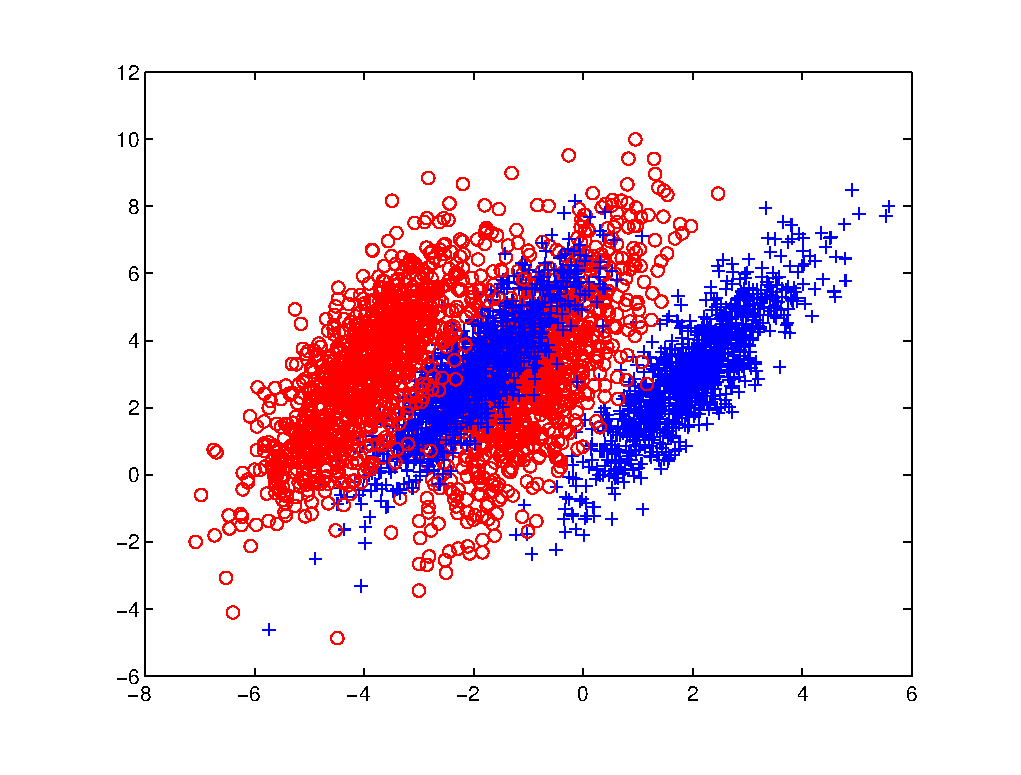
\includegraphics[width=2cm]{3_review/figures/classification/pbt-simulation/pbt_tree_1.eps}};
      \edge node[auto=right] {};
      [.\node{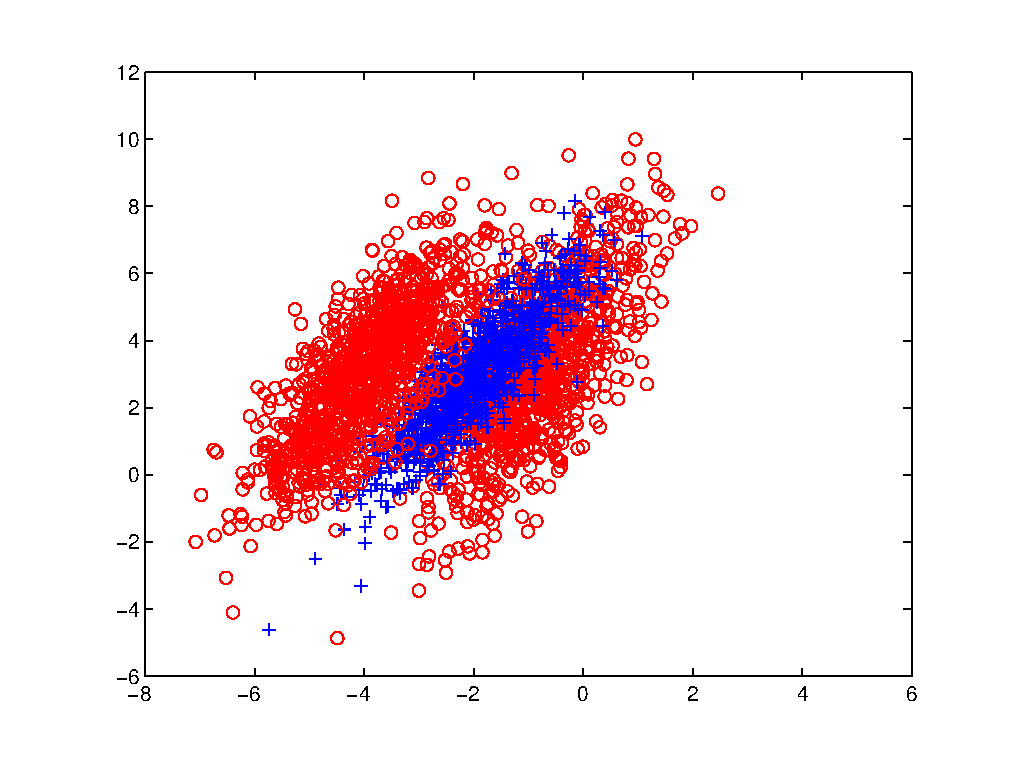
\includegraphics[width=2cm]{3_review/figures/classification/pbt-simulation/pbt_tree_2_1.eps}};
      \edge node[auto=right] {};
      [.\node{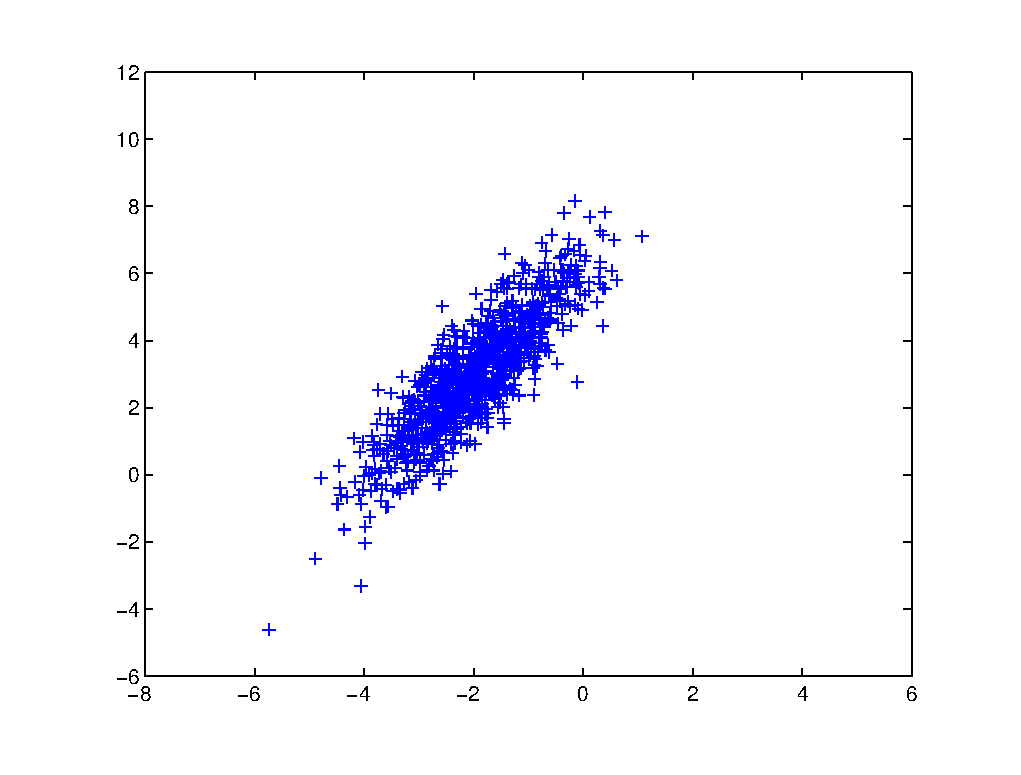
\includegraphics[width=2cm]{3_review/figures/classification/pbt-simulation/pbt_tree_3_2.eps}}; ]
      \edge node[auto=left] {};
      [.\node{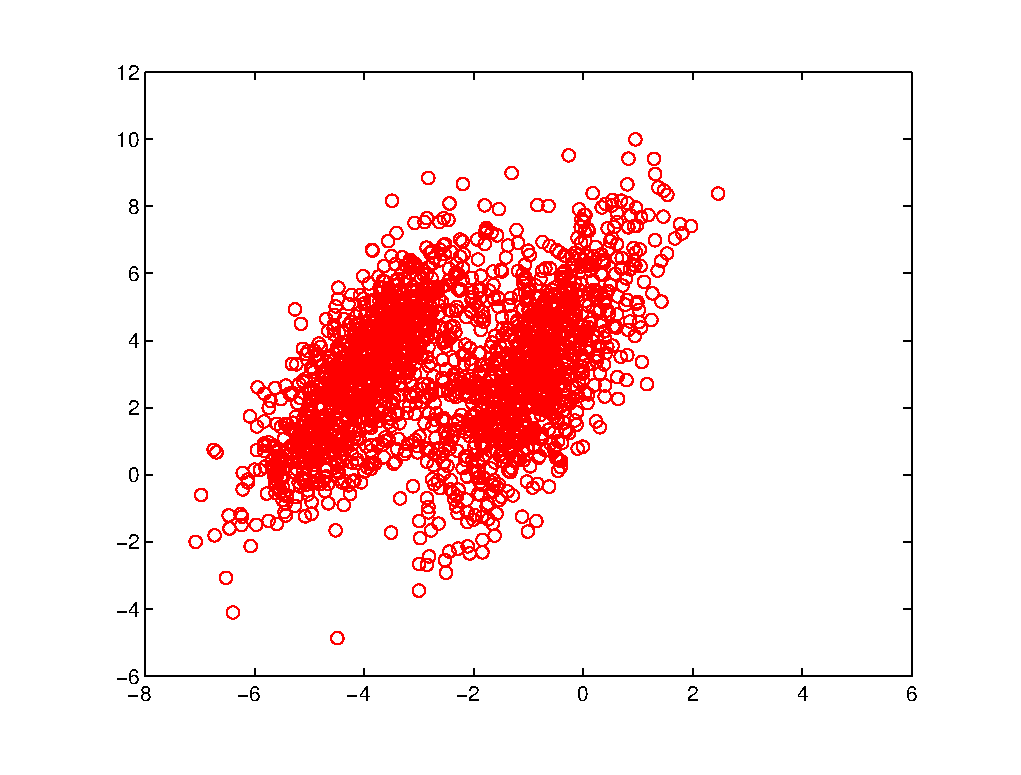
\includegraphics[width=2cm]{3_review/figures/classification/pbt-simulation/pbt_tree_3_1.eps}}; ]
      ]
      \edge node[auto=left] {};
      [.\node{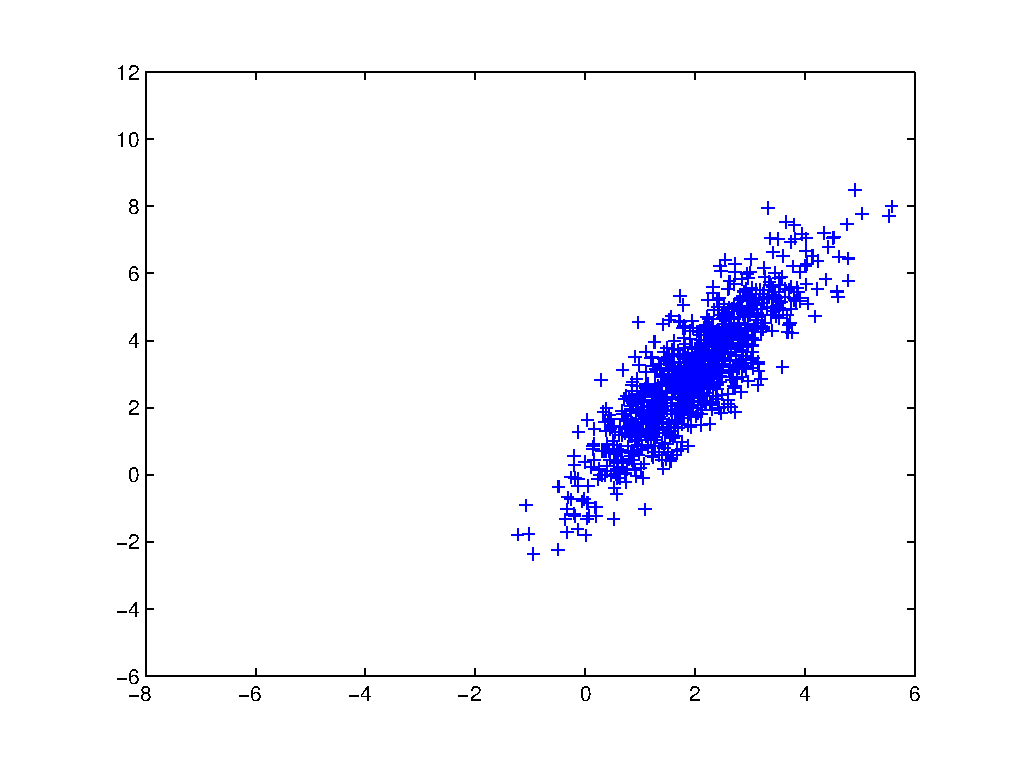
\includegraphics[width=2cm]{3_review/figures/classification/pbt-simulation/pbt_tree_2_2.eps}};
      ]
      ];
    \end{tikzpicture}
    \caption[Representation of the probabilistic boosting-tree.]{Representation
      of the capabilities of the probabilistic boosting-tree algorithm to split
      at each node of the tree the positive and negative samples.}
    \label{fig:pbtsim}
  \end{figure}

  Probabilistic boosting-tree is another ensemble learning classifier which
  shares principles with \ac{adb} but using them inside a decision
  tree~\cite{Tu2005}.
  In the training stage, the probabilistic boosting-tree method grows a
  decision tree and at each node, a strong classifier is learned in an almost
  comparable scheme to \ac{adb}.
  Once the strong learner is trained, the training set is split into two
  subsets which are used to train the next strong classifiers in the next
  descending nodes.
  Thus, three cases are conceivable to decide in which branch to propagate each
  sample training $\mathbf{x}_i$:

  \begin{itemize}
  \item if $q(+1, \mathbf{x}_i) - \frac{1}{2} > \epsilon$ then $\mathbf{x}_i$
    is propagated to the right branch set and a weight $w_i=1$ is assigned.
  \item if $q(-1, \mathbf{x}_i) - \frac{1}{2} > \epsilon$ then $\mathbf{x}_i$
    is propagated to the left branch set and a weight $w_i=1$ is assigned.
  \item else $\mathbf{x}_i$ will be propagated in both branches with $w_i=q(+1,
    \mathbf{x}_i)$ in the right branch and $w_i=q(-1, \mathbf{x}_i)$ in the
    left branch.
  \end{itemize}

  \noindent with $\mathbf{w} = w_i, i=\{1,\cdots,N\}$ corresponding to
  distribution of weights, $N$ the number of samples as in \ac{adb} and
  $q(\cdot)$ is defined as:

  \begin{eqnarray}
    q(+1, \mathbf{x}_i) & = & \frac{\exp(2H(\mathbf{x}_i))}{1+\exp(2H(\mathbf{x}_i))} \ , \label{eq:regada1} \\
    q(-1, \mathbf{x}_i) & = & \frac{\exp(-2H(\mathbf{x}_i))}{1+\exp(-2H(\mathbf{x}_i))} \ . \label{eq:regada2}
  \end{eqnarray}

  Employing such a scheme tends to divide the data in such a way that positive
  and negative samples are naturally split as shown in
  \acs{eq}\,\ref{fig:pbtsim}.
  In the classification stage, the unlabelled sample $\mathbf{x}$ is propagated
  through the tree, where at each node, it is classified by each strong
  classifier previously learned and where an estimation of the posterior
  distribution is computed.
  The posterior distribution corresponds to the sum of the posterior
  distribution at each node of the decision tree.
  The probabilistic boosting-tree classifier has been used
  in~\cite{Tiwari2009a,Tiwari2012,Tiwari2010,Viswanath2011}.

\item[] \textbf{Kernel method}
  A Gaussian process for classification is a kernel method in which it is
  assumed that the data can be represented by a single sample from a
  multivariate Gaussian distribution~\cite{Rasmussen2005}.
  In the case of linear logistic regression for classification, the posterior
  probability is expressed as:
  \begin{eqnarray}
    p(y_i|\mathbf{x}_i,\mathbf{w}) & = & \sigma(y_i f(\mathbf{x}_i)) \ , \label{eq:gp1} \\
    f(\mathbf{x}_i) & = & \mathbf{x}_i^{\text{T}} \mathbf{w} \ , \nonumber
  \end{eqnarray}

  \noindent where $\sigma(\cdot)$ is the logistic function and $\mathbf{w}$ are
  the parameters vector of the model.
  Thus, the classification using Gaussian processes is based on assigning a
  Gaussian process prior over the function $f(\mathbf{x})$ which is
  characterized by a mean function $\bar{f}$ and covariance function $K$.
  Therefore, in the training stage, the best mean and covariance functions have
  to be inferred in regard to our training data using a Newton optimization and
  a Laplacian approximation.
  The prediction stage is performed in two stages.
  First, for a new observation $\mathbf{x}_*$, the corresponding probability
  $p(f(\mathbf{x}_*)|f(\mathbf{x}))$ is computed such that:
  \begin{eqnarray}
    p(f(\mathbf{x}_*)|f(\mathbf{x})) & = & \mathcal{N}( K_*K^{-1}\bar{f}, K_{**}-K_*(K')^{-1}K_*^{\text{T}} ) \ , \nonumber \\
    K' & = & K + W^{-1} \ , \label{eq:gp2} \\
    W & = & \nabla \nabla \log p(\mathbf{y}|f(\mathbf{x})) \ , \nonumber
  \end{eqnarray}

  \noindent where $K_{**}$ is the covariance function $k(\mathbf{x}_*,
  \mathbf{x}_*)$ the testing sample $\mathbf{x}_*$, $K_{*}$ is the covariance
  function $k(\mathbf{x}, \mathbf{x}_*)$ of training-testing samples
  $\mathbf{x}$ and $\mathbf{x}_*$.
  Then, the function $f(\mathbf{x}_*)$ is squashed using the sigmoid function
  and the probability of the class membership is defined such that:

  \begin{equation}
    C(\mathbf{x}_*) = \sigma\left( \frac{\bar{f}(\mathbf{x_*})}{\sqrt{1+var(f(\mathbf{x}_*))}} \right) \ .
    \label{eq:gp3}
  \end{equation}

  Only \citeauthor{Kelm2007} used Gaussian process for classification of
  \ac{mrsi} data~\cite{Kelm2007}.

\item[] \textbf{Sparse kernel methods}
  In a classification scheme using Gaussian processes, when a prediction is
  performed, the whole training data are used to assign a label to the new
  observations.
  That is why this method is also called kernel method.
  Sparse kernel category is composed of methods which rely only on a few
  labelled observations of the training set to assign the label of new
  observations~\cite{Bishop2006}.

  \Acf{svm} is a sparse kernel method aiming at finding the best linear
  hyper-plane --- non-linear separation is discussed further --- which
  separates 2 classes such that the margin between the two classes is
  maximized~\cite{Vapnik1963}.
  The margin is in fact the region defined by 2 hyper-planes splitting the 2
  classes, such that there is no points lying in between.
  The distance between these 2 hyper-planes is equal to
  $\frac{2}{\|\mathbf{w}\|}$ where $\mathbf{w}$ is the normal vector of the
  hyper-plane splitting the classes.
  Thus, maximizing the margin is equivalent to minimizing the norm
  $\|\mathbf{w}\|$.
  Hence, this problem is solved by an optimization approach and formalized as:

  \begin{equation}
    \begin{aligned}
      & \argmin_{\mathbf{w}}
      & & \frac{1}{2} \| \mathbf{w}^2\| \ , \\
      & \text{subject to}
      & & y_i(\mathbf{w}.\mathbf{x}_i - b) \geq 1, \; i = \{ 1, \ldots, N \} \ ,
    \end{aligned}
    \label{eq:svm1}
  \end{equation}

  \noindent where $\mathbf{x}_i$ is a training sample with is corresponding
  class label $y_i$.
  From \acs{eq}\,\eqref{eq:svm1}, it is important to notice that only few
  points from the set of $N$ points are selected which later define the
  hyper-plane.
  This constraint is imposed in the optimization problem using Lagrange
  multipliers $\boldsymbol{\alpha}$.
  All points which are not lying on the margin are assigned a corresponding
  $\alpha_i = 0$, which is formalized as \acs{eq}\,\eqref{eq:svm2}.

  \begin{equation}
    \arg\min_{\mathbf{w},b } \max_{\boldsymbol{\alpha}\geq 0 } \left\{ \frac{1}{2}\|\mathbf{w}\|^2 - \sum_{i=1}^{n}{\alpha_i[y_i(\mathbf{w}\cdot \mathbf{x_i} - b)-1]} \right\} \ .
    \label{eq:svm2}
  \end{equation}

  The different parameters are inferred using quadratic programming.
  This version of \ac{svm} is known as hard-margin since no points can lie in
  the margin area.
  However, it is highly probable not to find any hyper-plane splitting the
  classes such as specified previously.
  Thus, a soft-margin optimization approach has been
  proposed~\cite{Cortes1995}, where points have the possibility to lie on the
  margin but at the cost of a penalty $\xi_i$ which is minimized in the
  optimization process such that:

  \begin{equation}
    \small
    \arg\min_{\mathbf{w},\mathbf{\xi}, b } \max_{\boldsymbol{\alpha},\boldsymbol{\beta} } \left\{ \frac{1}{2}\|\mathbf{w}\|^2+C \sum_{i=1}^n \xi_i - \sum_{i=1}^{n}{\alpha_i[y_i(\mathbf{w}\cdot \mathbf{x_i} - b) -1 + \xi_i]} - \sum_{i=1}^{n} \beta_i \xi_i \right\} \ .
  \end{equation}

  The decision to assign the label to a new observation $\mathbf{x}_i$ is taken
  such that:

  \begin{equation}
    C(\mathbf{x}_i) = \sign \left( \sum_{n=1}^{N} \alpha_n (\mathbf{x}_n . \mathbf{x}_i) + b_0 \right) \ ,
    \label{eq:svmdec}
  \end{equation}

  \noindent where $\mathbf{x}_n|n=\{1,\cdots,S\}$, $S$ being the support vectors.

  \ac{svm} can also be used as a non-linear classifier by performing a Kernel
  trick~\cite{Boser1992}.
  The original data $\mathbf{x}$ is projected to a high-dimensional space in
  which it is assumed that a linear hyper-plane splits the 2 classes.
  Different kernels are popular such as the \ac{rbf} kernel, polynomial
  kernels, or sigmoid kernels.
  In \ac{cad} for \ac{cap} systems, \ac{svm} is the most popular classification
  method and has been used in a multitude of research
  works~\cite{Artan2009,Artan2010,Chan2003,Litjens2011,Litjens2012,Liu2013,Lopes2011,Niaf2011,Niaf2012,Ozer2009,Ozer2010,Parfait2012,Peng2013,Sung2011,Tiwari2012,Vos2008,Vos2008a,Vos2010,Vos2012,giannini2015fully,trigui2017automatic,lehaire2014computer,khalvati2015automated,chung2015prostate}.

  \Acf{rvm} is a sparse version of Gaussian process previously presented,
  proposed in~\cite{Tipping2001}.
  \ac{rvm} is identical to a Gaussian process with the following covariance
  function~\cite{Quinonero-Candela2002}:

  \begin{equation}
    K_{RVM}(\mathbf{x}_p,\mathbf{x}_q) = \sum_{j=1}^{M} \frac{1}{\alpha_j} \Phi_j ( \mathbf{x}_p ) \Phi_j ( \mathbf{x}_q ) \ ,
    \label{eq:rvm}
  \end{equation}

  \noindent where $\phi(\cdot)$ is a Gaussian basis function,
  $\mathbf{x}_i|i=\{1,\cdots,N\}$ are the $N$ training points, and
  $\boldsymbol{\alpha}$ are the weights vector.
  As mentioned in~\cite{Quinonero-Candela2002}, the sparsity regarding the
  relevance vector arises for some $j$, the weight $\alpha_j^{-1} = 0$.
  The set of weights $\boldsymbol{\alpha}$ is inferred using the expectation
  maximization algorithm.
  \citeauthor{Ozer2010} used of \ac{rvm} and make a comparison with \ac{svm}
  for the task of \ac{cap} detection~\cite{Ozer2009,Ozer2010}.

\item[] \textbf{Neural network}
  Multilayer perceptron is a feed-forward neural network considered as the most
  successful model of this kind in pattern recognition~\cite{Bishop2006}.
  The most well known model used is based on 2 layers where a prediction of an
  observation is computed as:

  \begin{equation}
    C(\mathbf{x}_n,w_{ij}^{(1)},w_{kj}^{(2)}) = \sigma \left[ \sum_{j=0}^{M} w_{kj}^{(2)} \  h \left( \sum_{i=0}^{D} w_{ij}^{(1)} x_{in} \right) \right] \ ,
    \label{eq:annmlp}
  \end{equation}

  \noindent where $h(\cdot)$ and $\sigma(\cdot)$ are 2 activation functions
  usually non-linear, $w_{ij}^{(1)}$ and $ w_{kj}^{(2)}$ are the weights
  associated with the linear combination with the input feature $\mathbf{x}_n$
  and the hidden unit.

  \input{3_review/fig-NN-1.tex}

  A graphical representation of this network is presented in \acs{eq}\,\ref{fig:mlp}.
  Relating \acs{fig}\,\ref{fig:mlp} with \acs{eq}\,\eqref{eq:annmlp}, it can be
  noted that this network is composed of some successive non-linear mapping of
  the input data.
  First, a linear combination of the input vector $\mathbf{x}_n$ is mapped into
  some hidden units through a set of weights $w_{ij}^{(1)}$.
  This combination becomes non-linear by the use of the activation function
  $h(\cdot)$ which is usually chosen to be a sigmoid function.
  Then, the output of the networks consists of a linear combination of the
  hidden units and the set of weights $w_{kj}^{(2)}$.
  This combination is also mapped non-linearly using an activation function
  $\sigma(\cdot)$ which is usually a logistic function.
  Thus, the training of such a network resides in finding the best weights
  $w_{ij}^{(1)}$ and $ w_{kj}^{(2)}$ which model the best the training data.
  The error of this model is computed as:

  \begin{equation}
    E(w_{ij}^{(1)},w_{kj}^{(2)}) = \frac{1}{2} \sum_{n=1}^{N} \left( C(\mathbf{x}_n,w_{ij}^{(1)},w_{kj}^{(2)}) - y(\mathbf{x}_n) \right) ^{2} \ ,
    \label{eq:mlpcost}
  \end{equation}

  \noindent where $\mathbf{x}_n|n=\{1,\cdots,N\}$ are the $N$ training vectors
  with their corresponding class label $y(\mathbf{x}_n)$.

  Therefore, the best set of weights is inferred in an optimization framework
  where the error $E(\cdot)$ needs to be minimized.
  This optimization is performed using a gradient descent method where the
  derivative of \acs{eq}\,\eqref{eq:mlpcost} is computed using the
  back-propagation algorithm proposed by~\cite{Rumelhart1988}.
  This type of network has been used multiple
  times~\cite{Matulewicz2013,Parfait2012,trigui2017automatic,trigui2016classification,rampun2016computer}.

  \input{3_review/fig-NN-2.tex}

  Probabilistic neural networks are another type of feed-forward networks which
  is derived from the multilayer perceptron case and has been proposed
  by~\cite{Specht1988}.
  This classifier is modelled by changing the activation function $h(\cdot)$ in
  \acs{eq}\,\eqref{eq:annmlp} to an exponential function such that:

  \begin{equation}
    h(\mathbf{x}_n) = \exp \left( - \frac{ (\mathbf{w}_j - \mathbf{x})^{\text{T}}(\mathbf{w}_j - \mathbf{x}) }{2\sigma^2} \right) \ ,
    \label{eq:pnn1}
  \end{equation}

  \noindent where $\sigma$ is a free parameter set by the user.

  The other difference of the probabilistic neural networks compared with the
  multilayer perceptron networks resides in the architecture as shown in
  \acs{fig}\,\ref{fig:pnn}.
  This network is formed by 2 hidden layers.
  The first hidden layer consists of the pattern layer, in which the mapping is
  done using \acs{eq}\,\eqref{eq:pnn1}.
  This pattern layer is sub-divided into a number of groups corresponding to
  the number of classes.
  The second hidden layer corresponds to the summation layer which simply sums
  the output of each sub-group of the pattern layer.
  This method is used in~\cite{Ampeliotis2007,Ampeliotis2008,Viswanath2011}.

\item[] \textbf{Graphical model classifiers}
  \Ac{mrf} is used as a lesion segmentation method to detect \ac{cap}.
  First, let define $s$ as a pixel which belongs to a certain class denoted by
  $\omega_s$.
  The labelling process is defined as $\omega = \{\omega_s, s \in I\}$ where
  $I$ is the set of all the pixels inside the image.
  The observations corresponding to \ac{si} in the image are noted $\mathcal{F}
  = \{ f_s | s \in I \}$.
  Thus, the image process $\mathcal{F}$ represents the deviation from the
  labelling process $\omega$~\cite{Kato2001}.
  Hence, lesion segmentation is equivalent to estimating the best
  $\hat{\omega}$ which maximizes the posterior probability
  $p(\omega|\mathcal{F})$.
  Thus, using a Bayesian approach, this problem is formulated such that:

  \begin{equation}
    p(\omega|\mathcal{F}) = \argmax_{\omega} \prod_{s \in I} p(f_s | \omega_s) p(\omega) \ .
    \label{eq:mrf1}
  \end{equation}

  It is generally assumed that $p(f_s | \omega_s)$ follows a Gaussian
  distribution and that the pixels classes $\lambda = \{1,2\}$ for a binary
  classification are characterized by their respective mean $\mu_{\lambda}$ and
  standard deviation $\sigma_{\lambda}$.
  Then, $\omega$ is a Markov random field, thus:

  \begin{equation}
    p(\omega) =  \frac{1}{Z} \exp\left( -U(\omega) \right)  \ ,
    \label{eq:mrf2}
  \end{equation}

  \noindent where $Z$ is a normalization factor to obtain a probability value,
  $U(\cdot)$ is the energy function.

  Thus, the segmentation problem is solved as an optimization problem where the
  energy function $U(\cdot)$ has to be minimized.
  There are different possibilities to define the energy function $U(\cdot)$.
  However, it is common to define the energy function such that it combines two
  types of potential function: (i) a local term relative to the pixel itself
  and (ii) a smoothing prior which embeds neighbourhood information which
  penalizes the energy function affecting the region homogeneity.
  This optimization of such a function can be performed using an algorithm such
  as iterated conditional modes~\cite{Kato2001}.
  \citeauthor{Liu2009} and \citeauthor{Ozer2010} used \ac{mrf} as an
  unsupervised method to segment lesions in \ac{mpmri}
  images~\cite{Liu2009,Ozer2010}.
  \citeauthor{Artan2010} and \citeauthor{chung2015prostate} used conditional
  random fields instead of \ac{mrf} for \ac{mri}
  segmentation~\cite{Artan2009,Artan2010,chung2015prostate}.
  The difference between these 2 methods resides in the fact that conditional
  probabilities are defined such as:

  \begin{equation}
    p(\omega|\mathcal{F}) =  \frac{1}{Z} \exp \left[ - \sum_{s \in I} V_{C1}(\omega_s|\mathcal{F}) - \sum_{\{s,r\} \in C } V_{C2} (\omega_s,\omega_r|\mathcal{F})  \right] \ .
    \label{eq:crf}
  \end{equation}

  \noindent $V_{C1}(\cdot)$ is the state (or partition) feature function and
  $V_{C2}(\cdot)$ is the transition (or edge) feature
  function~\cite{Kato2012}.

\end{enumerate}

Classification methods used to distinguish \ac{cap} from healthy tissue in in
\ac{cad} systems are summarized in \acs{tab}~\ref{tab:class}.

\begin{table}
  \caption{Overview of the classifiers used in \acs*{cad} systems.}
  \scriptsize
  \begin{tabularx}{\textwidth}{l >{\raggedleft\arraybackslash}X@{}}
    \toprule
    \textbf{Classifier} & \textbf{References} \\
    \midrule
    \textbf{Rule-based method:} & \cite{Lv2009,Puech2009} \\ \\ [-1.5ex]
    \textbf{Clustering methods:} & \\
    \quad $k$-means clustering & \cite{Tiwari2007,Tiwari2008,Tiwari2009} \\
    \quad \acs{knn} & \cite{Litjens2012,Niaf2011,Niaf2012,rampun2016computerb} \\ \\ [-1.5ex]
    \textbf{Linear model classifiers:} & \\
    \quad \acs{lda} & \cite{Antic2013,Chan2003,Litjens2014,Niaf2011,Niaf2012,Vos2012} \\
    \quad Logistic regression & \cite{Kelm2007,Langer2009,lehaire2014computer,rampun2015computer} \\ \\ [-1.5ex]
    \textbf{Non-linear classifier:} & \\
    \quad \acs{qda} & \cite{Viswanath2012} \\ \\ [-1.5ex]
    \textbf{Probabilistic classifier:} & \\
    \quad Naive Bayes & \cite{Giannini2013,Mazzetti2011,Niaf2011,Niaf2012,cameron2014multiparametric,cameron2016maps,rampun2015classifying,rampun2016computerb,rampun2015computer,rampun2016computer} \\ \\ [-1.5ex]
    \textbf{Ensemble learning classifiers:} & \\
    \quad \acs*{adb} & \cite{Litjens2014,Lopes2011} \\
    \quad \acs*{gb} & \cite{Lemaitre2016thesis} \\
    \quad \acs*{rf} & \cite{Kelm2007,Litjens2014,Tiwari2012,Tiwari2013,Viswanath2009,trigui2017automatic,trigui2016classification,samarasinghe2016semi,rampun2015classifying,rampun2016computerb,rampun2015computer,rampun2016computer,Lemaitre2016thesis} \\
    \quad Probabilistic boosting tree & \cite{Tiwari2009,Tiwari2010,Tiwari2012} \\ \\ [-1.5ex]
    \textbf{Kernel method:} & \\
    \quad Gaussian processes & \cite{Kelm2007} \\ \\ [-1.5ex]
    \textbf{Sparse kernel methods:} & \\
    \quad \acs{svm} & \cite{Artan2009,Artan2010,Chan2003,Litjens2011,Litjens2012,Liu2013,Lopes2011,Niaf2011,Niaf2012,Ozer2009,Ozer2010,Parfait2012,Peng2013,Sung2011,Tiwari2012,Vos2008,Vos2008a,Vos2010,Vos2012,giannini2015fully,trigui2017automatic,lehaire2014computer,khalvati2015automated,chung2015prostate} \\
    \quad \acs{rvm} & \cite{Ozer2009,Ozer2010} \\ \\ [-1.5ex]
    \textbf{Neural network:} & \\
    \quad Multiple layer perceptron & \cite{Matulewicz2013,Parfait2012,trigui2017automatic,trigui2016classification,rampun2016computer} \\
    \quad Probabilistic neural network & \cite{Ampeliotis2007,Ampeliotis2008,Viswanath2011} \\ \\ [-1.5ex]
    \textbf{Graphical model classifiers:} & \\
    \quad Markov random field & \cite{Liu2009,Ozer2010} \\
    \quad Conditional random field & \cite{Artan2009,Artan2010,chung2015prostate} \\
    \bottomrule
  \end{tabularx}
  \label{tab:class}
\end{table}

\subsection{Model validation} \label{subsec:chp3:img-clas:CADX-val}

\begin{table}
  \caption{Overview of the model validation techniques used in \acs*{cad} systems.}
  \centering
  % \renewcommand{\arraystretch}{1.5}
  \begin{tabularx}{\textwidth}{@{}l >{\raggedleft\arraybackslash}X@{}}
    \toprule
    \textbf{Model validation techniques} & \textbf{References} \\ \\ [-1.5ex]
    \midrule
    \quad \acs*{loo} & \cite{Ampeliotis2007,Ampeliotis2008,Antic2013,Artan2009,Artan2010,Chan2003,Giannini2013,Kelm2007,Litjens2012,Litjens2014,Mazzetti2011,Niaf2011,Niaf2012,Ozer2009,Ozer2010,Peng2013,Puech2009,Tiwari2013,Viswanath2011,Vos2008,Vos2008,Vos2010,cameron2016maps,cameron2014multiparametric,lehaire2014computer,khalvati2015automated,chung2015prostate} \\ \\ [-1.5ex]
    \quad \acs*{kcv} & \cite{Litjens2011,Parfait2012,Tiwari2009,Tiwari2009a,Tiwari2010,Tiwari2012,Viswanath2012,Viswanath2009,Vos2012,trigui2016classification,trigui2017automatic,rampun2015classifying,rampun2015computer,rampun2016computer,rampun2016computerb,rampun2016quantitative} \\ \\ [-1.5ex]
    \bottomrule
  \end{tabularx}
\label{tab:valmod}
\end{table}

In pattern recognition, the use of model validation techniques to assess the
performance of a classifier plays an important role for reporting results.
Two techniques are broadly used in the development of \ac{cad} systems and are
summarized in \acs{tab}~\ref{tab:valmod}.
The most popular technique used in \ac{cad} systems is the \ac{loo} technique.
From the whole data, one patient is kept for validation and the other cases are
used for training.
This manipulation is repeated until each patient has been used for validation.
This technique is popular when working with a limited number of patients,
allowing to train on representative number of cases even with a small dataset.
However, \ac{loo} cross-validation suffers from a large variance and is
considered as an unreliable estimate~\cite{Efron1983}.

The other technique is the \ac{kcv} technique which is based on splitting the
dataset into $k$ subsets where the samples are randomly selected.
Then, one fold is kept for testing and the remaining subsets are used for
training.
The classification is then repeated as in the \ac{loo} technique.
In fact \ac{loo} is a particular case of \ac{kcv} when $k$ equals the number of
patients.
In the reviewed papers, the typical values used for $k$ has been set to three
and five.
\Ac{kcv} is regarded as more appropriate than \ac{loo}, but the number of
patients in the dataset needs to be large enough for the results to be
meaningful.

\subsection{Evaluation measures} \label{subsec:chp3:img-clas:eval-mea}

\begin{table}
  \caption{Overview of the evaluation metrics used in \acs*{cad} systems.}
  \begin{tabularx}{\textwidth}{@{}l >{\raggedleft\arraybackslash}X@{}}
    \toprule
    \textbf{Evaluation metrics} & \textbf{References} \\
    \midrule
    \quad Accuracy & \cite{Artan2009,Artan2010,Liu2009,Sung2011,Tiwari2012} \\
    \quad Sensitivity - Specificity & \cite{Artan2009,Artan2010,Giannini2013,Liu2009,Lopes2011,Mazzetti2011,Ozer2009,Ozer2010,Parfait2012,Peng2013,Tiwari2008,Tiwari2009,Viswanath2008,Viswanath2008a,trigui2016classification,trigui2017automatic,samarasinghe2016semi,cameron2014multiparametric,cameron2016maps,khalvati2015automated} \\
    \quad \acs*{roc} - \acs*{auc} & \cite{Ampeliotis2008,Antic2013,Chan2003,Giannini2013,Kelm2007,Langer2009,Liu2013,Lopes2011,Lv2009,Matulewicz2013,Mazzetti2011,Niaf2011,Niaf2012,Peng2013,Tiwari2009a,Tiwari2010,Tiwari2012,Tiwari2013,Viswanath2009,Viswanath2011,Viswanath2012,Vos2008,Vos2008a,Vos2010,giannini2015fully,lehaire2014computer,rampun2015classifying,rampun2015computer,rampun2016computer,rampun2016computerb,rampun2016quantitative} \\
    \quad \acs*{froc} & \cite{Litjens2011,Litjens2012,Vos2012} \\
    \quad Dice's coefficient & \cite{Artan2009,Artan2010,Liu2009,Ozer2009} \\
    \bottomrule
  \end{tabularx}
\label{tab:evatec}
\end{table}

Several metrics are used in order to assess the performance of a classifier and
are summarized in \acs{tab}~\ref{tab:evatec}.
Voxels in the \ac{mri} image are classified into healthy or malign tissue and
compared with a ground-truth.
This allows to compute a confusion matrix by counting true positive (TP), true
negative (TN), false positive (FP), and false negative (FN) samples.
From this analysis, different statistics are extracted.

The first statistic used is the accuracy which is computed as the ratio of true
detection to the number of samples.
However, depending on the strategy employed in the \ac{cad} work-flow, this
statistic is highly biased by a high number of true negative samples which
boost the accuracy score overestimating the actual performance of the
classifier.
That is why, the most common statistics computed are sensitivity and
specificity defined in \acs{eq}\,\eqref{eq:sens} and \acs{eq}\,\eqref{eq:spec},
respectively.
The metrics give a full overview of the performance of the classifier.

\begin{equation}
  \text{SE} = \frac{\text{TP}}{\text{TP} + \text{FN}} \ ,
  \label{eq:sens}
\end{equation}

\begin{equation}
  \text{SP} = \frac{\text{TN}}{\text{TN} + \text{FP}} \ .
  \label{eq:spec}
\end{equation}

These statistics are also used to compute the \ac{roc} curves~\cite{Metz2006},
which give information about voxel-wise classification.
This analysis represents graphically the sensitivity as a function of $(1 -
\text{specificity})$, which is in fact the false positive rate, by varying the
discriminative threshold of the classifier.
By varying this threshold, more true negative samples are found but often at
the cost of detecting more false negatives.
However, this fact is interesting in \ac{cad} since it is possible to obtain a
high sensitivity and to ensure that no cancers are missed even if more false
alarms have to be investigated or the opposite.
A statistic derived from \ac{roc} analysis is the \acf{auc} which corresponds
to the area under the \ac{roc} and is a measure used to make comparisons
between models.

The \acf{froc} extends the \ac{roc} analysis but to a lesion-based level.
The same confusion matrix is computed where the sample are not pixels but
lesions.
However, it is important to define what is a true positive sample in that case.
Usually, a lesion is considered as a true positive sample if the region
detected by the classifier overlaps ``sufficiently'' the one delineated in the
ground-truth.
However, ``sufficiently'' is a subjective measure defined by each researcher
and can correspond to one pixel only.
However, an overlap of \SIrange{30}{50}{\percent} is usually adopted.
Finally, in addition to the overlap measure, the Dice's coefficient is often
computed to evaluate the accuracy of the lesion localization.
This coefficient consists of the ratio between twice the number of pixels in
common and the sum of the pixels of the lesions in the ground-truth $\text{GT}$
and the output of the classifier $\text{S}$, defined as shown in
\acs{eq}\,\eqref{eq:dice}.

\begin{equation}
  Q_D = \frac{2 | \text{GT} \cap \text{S} |}{| \text{GT} | + | \text{S} |} \ .
  \label{eq:dice}
\end{equation}


\section{Discussion}\label{sec:chp3:dis}

\subsection{Results reported}\label{subsec:chp3:dis:res}

As discussed previously in \ac{sec}\,\ref{subsec:chp3:img-clas:eval-mea},
different metrics have been used to report results.
A comparison of the different methods reviewed is given depending on the metric
used in field of research and also the type of \ac{mri} scanner used,
i.e. \SI{1.5}{\tesla} or \SI{3}{\tesla}.
For each field, the \textit{best classification performance} obtained in each
study have been reported in these figures.
The results in terms of \ac{auc}-\ac{roc} are depicted in
\acs{fig}\,\ref{fig:auc}.
The results vary from \SIrange{71}{97}{\percent} for some experiments with a
\SI{1.5}{\tesla} \ac{mri} scanner and from \SIrange{77}{95}{\percent} with a
\SI{3}{\tesla} \ac{mri} scanner.

The results in regard of sensitivity and specificity are reported in
\acs{fig}\,\ref{fig:sensspec}.
In the case that the data have been collected with a \SI{1.5}{\tesla} \ac{mri}
scanner, the sensitivity ranges from \SIrange{74}{100}{\percent} and the
specificity from \SIrange{43}{93}{\percent}.
For the experiments carried out with a \SI{3}{\tesla} \ac{mri} scanner, the
sensitivity varies from \SIrange{60}{99}{\percent} and the specificity from
\SIrange{66}{100}{\percent}.
Four studies also use \ac{froc} analysis to report their results and are
reported in \ac{fig}\,\ref{fig:froc}.

\begin{figure}
  \centering
  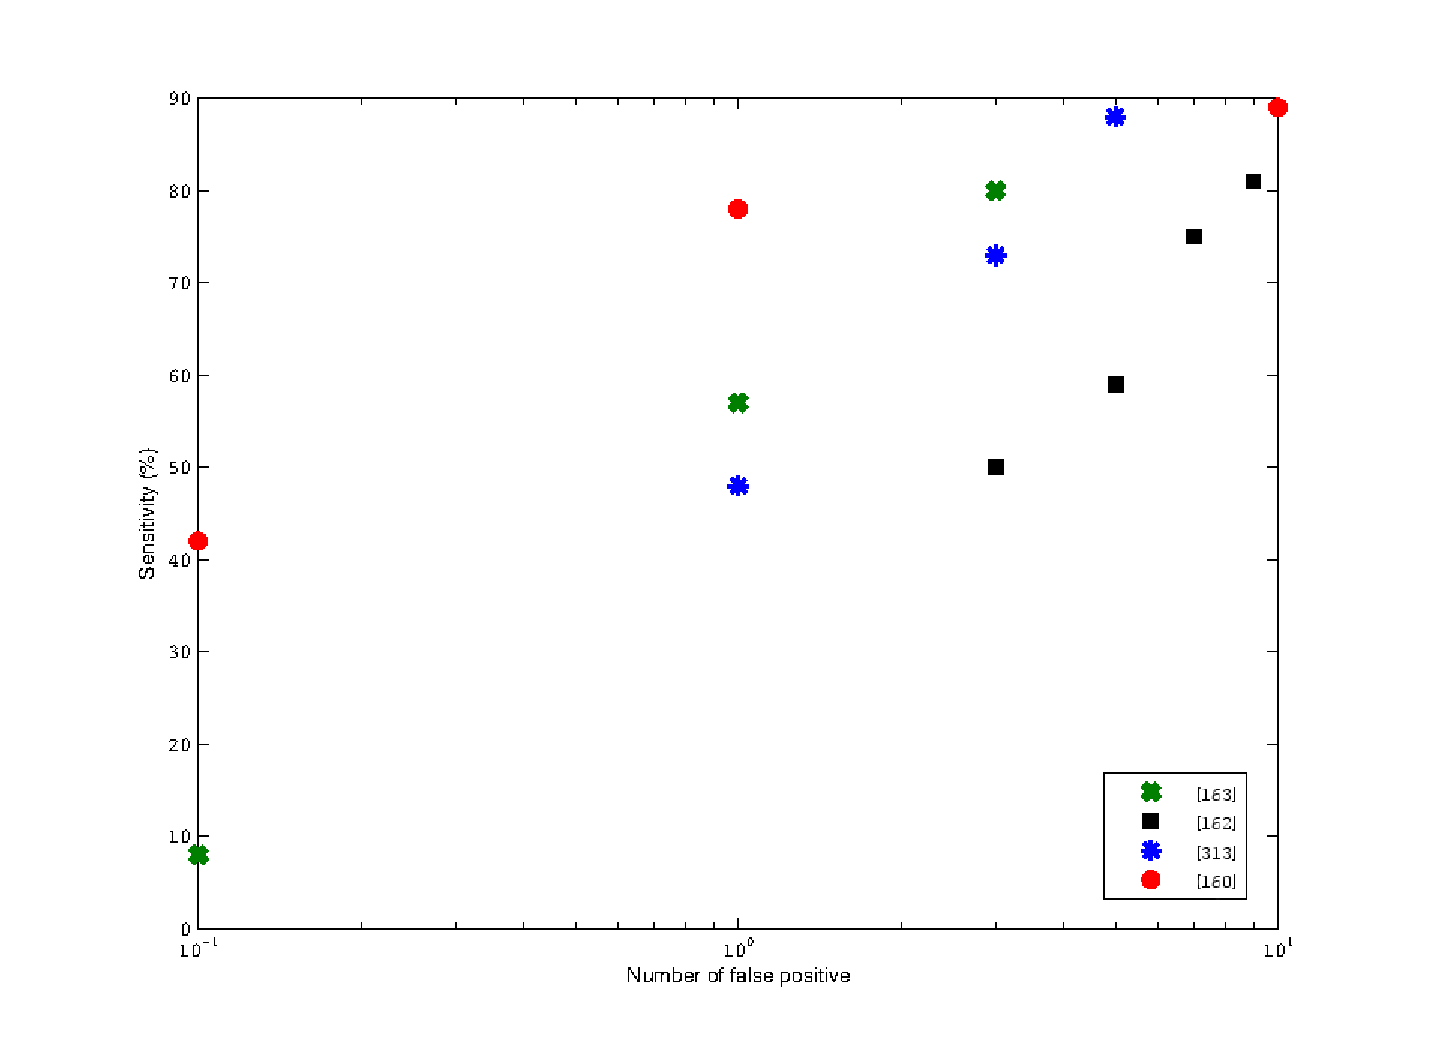
\includegraphics[width=.8\linewidth]{3_review/figures/results/froc.eps}
  \caption{Comparison in terms of \acs*{froc} of the methods using data from
    \SI{3}{\tesla} \acs*{mri} scanner.}
  \label{fig:froc}
\end{figure}

\begin{figure}
  \centering
 % \hspace{\fill}
  \subfloat[]{
    \label{fig:auc15}
    \begin{tikzpicture}[scale=.7,every node/.style={scale=0.7}]

      \def\labels{
        {\color{blue}\cite{Ampeliotis2008}},
        {\color{blue}\cite{Antic2013}},
        {\color{blue}\cite{Chan2003}},
        {\color{blue}\cite{Giannini2013}},
        {\color{blue}\cite{Langer2009}},
        {\color{blue}\cite{Lopes2011}},
        {\color{blue}\cite{Lv2009}},
        {\color{blue}\cite{Niaf2011}},
        {\color{blue}\cite{Niaf2012}},
        {\color{blue}\cite{Tiwari2009a}},
        {\color{blue}\cite{Tiwari2010}},
        {\color{blue}\cite{Tiwari2012}},
        {\color{blue}\cite{Tiwari2013}},
        {\color{blue}\cite{Vos2008}},
        {\color{blue}\cite{Vos2010}},
        {\color{blue}\cite{lehaire2014computer}},
        {\color{blue}\cite{giannini2015fully}},
        {\color{blue}\cite{Mazzetti2011}},
        {\color{blue}\cite{Puech2009}},
        {\color{blue}\cite{Vos2008a}},
        {\color{blue}\cite{rampun2016computerb}},
        {\color{blue}\cite{rampun2016computer}}
      }

      \def\reward{90,94,84,87,71,93,97,87,87,84,91,90,85,91,97,75,91,92,77,90,93,93}
      \def\dbSize{25,53,15,10,25,27,55,23,30,15,19,36,29,29,29,35,56,29,100,10,45,45}
      \def\dbClass{1,2,1,1,1,1,2,1,1,1,1,1,1,1,1,1,2,1,3,1,2,2}
      \def\cZoom{3}
      \def\percentageLabelAngle{90}
      \def\nbeams{22}
      \pgfmathsetmacro\beamAngle{(360/\nbeams)}
      \pgfmathsetmacro\halfAngle{(180/\nbeams)}
      \pgfmathsetmacro\globalRotation{\halfAngle}

      % draw the radiants
      \foreach \n  [count=\ni] in \labels
      {
        \pgfmathsetmacro\cAngle{{(\ni*(360/\nbeams))+\globalRotation}}
        \draw(\cAngle:{\cZoom*1.15})  node[fill=white] {\n};
        \draw [thin] (0,0) -- (\cAngle:{\cZoom*1}) ;

      }

      % draw the % rings
      \foreach \x in {12.5,25, ...,100}
      \draw [thin,color=gray!50] (0,0) circle [radius={\cZoom*\x/100}];

      \foreach \x in {50,75,100}
      {
        \draw [thin,color=black!50] (0,0) circle [radius={\cZoom/100*\x}];
        \foreach \a in {0, 180} \draw ({\percentageLabelAngle+\a}:{\cZoom*0.01*\x}) node  [inner sep=0pt,outer sep=0pt,fill=white,font=\fontsize{8}{8.5}\selectfont]{$\x\%$};
      }

      % draw the path of the percentages
      \def\aux{{\reward}}
      \pgfmathsetmacro\origin{\aux[\nbeams-1]}
      \draw [semiAuto, thick] (\globalRotation:{\cZoom*\origin/100}) \foreach \n  [count=\ni] in \reward { -- ({(\ni*(360/\nbeams))+\globalRotation}:{\cZoom*\n/100}) } ;

      % label all the percentags
      \foreach \n [count=\ni] in \dbSize
      {
        \pgfmathsetmacro\cAngle{{(\ni*(360/\nbeams))+\globalRotation}}
        \pgfmathsetmacro\nreward{\aux[\ni-1]}
        \draw (\cAngle:{\cZoom*1.5}) node[align=center] {{\color{semiAuto}\nreward $\%$} \\ {\color{red}\n} };
      } ;

      % draw the database rose
      \def\dbScale{\9}
      \foreach \n [count=\ni] in \dbClass
      \filldraw[fill=red!20!white, draw=red!50!black]
      (0,0) -- ({\ni*(360/\nbeams)-\halfAngle+\globalRotation}:{\cZoom*\n/9}) arc ({\ni*(360/\nbeams)-\halfAngle+\globalRotation}:{\ni*(360/\nbeams)+\halfAngle+\globalRotation}:{\cZoom*\n/9}) -- cycle;
      \foreach \x in {1,2,3}
      \draw [thin,color=red!50!black,dashed] (0,0) circle [radius={\cZoom*\x/9}];

      %% draw the domain of each class
      \def\puta{17/0/{Multiparametric},
        5/17/{Monoparametric}}

      \foreach \numElm/\contadorQueNoSeCalcular/\name [count=\ni] in \puta
      {

        \pgfmathsetmacro\initialAngle{(\contadorQueNoSeCalcular*\beamAngle)+\halfAngle+\globalRotation}
        \pgfmathsetmacro\finalAngle  {((\numElm+\contadorQueNoSeCalcular)*\beamAngle)+\halfAngle+\globalRotation}
        \pgfmathsetmacro\l  {\cZoom*1.65+.3pt}
        \draw (\initialAngle:{\cZoom*1.7}) -- (\initialAngle:{\cZoom*1.1});
        \draw [ |<->|,>=latex] (\initialAngle:\l) arc (\initialAngle:\finalAngle:\l) ;
        \pgfmathsetmacro\r  {\cZoom*1.65+.45pt}
        {\draw [decoration={raise=4pt,text along path,text={\name},text align={center}},decorate] (\finalAngle:\r) arc (\finalAngle:\initialAngle:\r);}
      }

    \end{tikzpicture}}\\
  \subfloat[]{
    \label{fig:auc30}
    \begin{tikzpicture}[scale=.7,every node/.style={scale=0.7}]

      \def\labels{
        {\color{blue}\cite{Litjens2014}},
        {\color{blue}\cite{Liu2013}},
        {\color{blue}\cite{Peng2013}},
        {\color{blue}\cite{Viswanath2009}},
        {\color{blue}\cite{Viswanath2011}},
        {\color{blue}\cite{khalvati2015automated}},
        {\color{blue}Our},
        {\color{blue}\cite{Viswanath2012}}
      }

      \def\reward{94,83,95,82,77,90,84,80}
      \def\dbSize{347,54,48,6,12,20,19,22}
      \def\dbClass{3,2,2,1,1,1,1,1}
      \def\cZoom{3}
      \def\percentageLabelAngle{90}
      \def\nbeams{8}
      \pgfmathsetmacro\beamAngle{(360/\nbeams)}
      \pgfmathsetmacro\halfAngle{(180/\nbeams)}
      \pgfmathsetmacro\globalRotation{\halfAngle}

      % draw the radiants
      \foreach \n  [count=\ni] in \labels
      {
        \pgfmathsetmacro\cAngle{{(\ni*(360/\nbeams))+\globalRotation}}
        \draw(\cAngle:{\cZoom*1.15})  node[fill=white] {\n};
        \draw [thin] (0,0) -- (\cAngle:{\cZoom*1}) ;

      }

      % draw the % rings
      \foreach \x in {12.5,25, ...,100}
      \draw [thin,color=gray!50] (0,0) circle [radius={\cZoom*\x/100}];

      \foreach \x in {50,75,100}
      {
        \draw [thin,color=black!50] (0,0) circle [radius={\cZoom/100*\x}];
        \foreach \a in {0, 180} \draw ({\percentageLabelAngle+\a}:{\cZoom*0.01*\x}) node  [inner sep=0pt,outer sep=0pt,fill=white,font=\fontsize{8}{8.5}\selectfont]{$\x\%$};
      }

      % draw the path of the percentages
      \def\aux{{\reward}}
      \pgfmathsetmacro\origin{\aux[\nbeams-1]}
      \draw [semiAuto, thick] (\globalRotation:{\cZoom*\origin/100}) \foreach \n  [count=\ni] in \reward { -- ({(\ni*(360/\nbeams))+\globalRotation}:{\cZoom*\n/100}) } ;

      % label all the percentags
      \foreach \n [count=\ni] in \dbSize
      {
        \pgfmathsetmacro\cAngle{{(\ni*(360/\nbeams))+\globalRotation}}
        \pgfmathsetmacro\nreward{\aux[\ni-1]}
        \draw (\cAngle:{\cZoom*1.5}) node[align=center] {{\color{semiAuto}\nreward $\%$} \\ {\color{red}\n} };
      } ;

      % draw the database rose
      \def\dbScale{\9}
      \foreach \n [count=\ni] in \dbClass
      \filldraw[fill=red!20!white, draw=red!50!black]
      (0,0) -- ({\ni*(360/\nbeams)-\halfAngle+\globalRotation}:{\cZoom*\n/9}) arc ({\ni*(360/\nbeams)-\halfAngle+\globalRotation}:{\ni*(360/\nbeams)+\halfAngle+\globalRotation}:{\cZoom*\n/9}) -- cycle;
      \foreach \x in {1,2,3}
      \draw [thin,color=red!50!black,dashed] (0,0) circle [radius={\cZoom*\x/9}];

      %% draw the domain of each class
      \def\puta{7/0/{Multiparametric},
        1/7/{Monoparametric}}

      \foreach \numElm/\contadorQueNoSeCalcular/\name [count=\ni] in \puta
      {

        \pgfmathsetmacro\initialAngle{(\contadorQueNoSeCalcular*\beamAngle)+\halfAngle+\globalRotation}
        \pgfmathsetmacro\finalAngle  {((\numElm+\contadorQueNoSeCalcular)*\beamAngle)+\halfAngle+\globalRotation}
        \pgfmathsetmacro\l  {\cZoom*1.65+.3pt}
        \draw (\initialAngle:{\cZoom*1.7}) -- (\initialAngle:{\cZoom*1.1});
        \draw [ |<->|,>=latex] (\initialAngle:\l) arc (\initialAngle:\finalAngle:\l) ;
        \pgfmathsetmacro\r  {\cZoom*1.65+.45pt}
        {\draw [decoration={raise=4pt,text along path,  text={\name},text align={center}},decorate] (\finalAngle:\r) arc (\finalAngle:\initialAngle:\r);}
      }

    \end{tikzpicture}
 }
  %\hspace{\fill}
  \caption[Results comparison from the state-of-the-art in terms of \acs*{auc}.]{Numerical and graphical comparison of the results in terms of \acs*{auc} for \SI{1.5}{\tesla}~\subref{fig:auc15} and \SI{3}{\tesla}~\subref{fig:auc30} \acs*{mri} scanners. The {\color{semiAuto}green} value represents the metric and are graphically reported in the {\color{semiAuto}green} curve in the center of the figure. The {\color{red}red} value and areas correspond to the number of patients in the dataset. The numbers between brackets in {blue\color{blue}} correspond to the reference as reported in \acs{tab}~\ref{tab:sumpap}.}
  \label{fig:auc}
\end{figure}

\begin{figure}%
 \centering
 \hspace*{\fill}
  \subfloat[]{
    \label{fig:sens15}
    \begin{tikzpicture}[scale=.5,every node/.style={scale=0.5}]

      \def\labels{
        {\color{blue}\cite{Artan2009}},
        {\color{blue}\cite{Artan2010}},
        {\color{blue}\cite{Giannini2013}},
        {\color{blue}\cite{Liu2009}},
        {\color{blue}\cite{Lopes2011}},
        {\color{blue}\cite{Ozer2009}},
        {\color{blue}\cite{Ozer2010}},
        {\color{blue}\cite{Tiwari2009a}},
        {\color{blue}\cite{Viswanath2008}},
        {\color{blue}\cite{Mazzetti2011}},
        {\color{blue}\cite{Puech2009}},
        {\color{blue}\cite{Tiwari2008}}
      }

      \def\reward{74,66,79,90,85,76,78,84,88,82,100,87}
      \def\dbSize{10,21,10,11,27,20,20,18,16,10,100,18}
      \def\dbClass{1,2,1,1,2,1,1,1,1,1,3,1}
      \def\cZoom{3}
      \def\percentageLabelAngle{90}
      \def\nbeams{12}
      \pgfmathsetmacro\beamAngle{(360/\nbeams)}
      \pgfmathsetmacro\halfAngle{(180/\nbeams)}
      \pgfmathsetmacro\globalRotation{\halfAngle}

      % draw the radiants
      \foreach \n  [count=\ni] in \labels
      {
        \pgfmathsetmacro\cAngle{{(\ni*(360/\nbeams))+\globalRotation}}
        \draw(\cAngle:{\cZoom*1.15})  node[fill=white] {\n};
        \draw [thin] (0,0) -- (\cAngle:{\cZoom*1}) ;

      }

      % draw the % rings
      \foreach \x in {12.5,25, ...,100}
      \draw [thin,color=gray!50] (0,0) circle [radius={\cZoom*\x/100}];

      \foreach \x in {50,75,100}
      {
        \draw [thin,color=black!50] (0,0) circle [radius={\cZoom/100*\x}];
        \foreach \a in {0, 180} \draw ({\percentageLabelAngle+\a}:{\cZoom*0.01*\x}) node  [inner sep=0pt,outer sep=0pt,fill=white,font=\fontsize{8}{8.5}\selectfont]{$\x\%$};
      }

      % draw the path of the percentages
      \def\aux{{\reward}}
      \pgfmathsetmacro\origin{\aux[\nbeams-1]}
      \draw [semiAuto, thick] (\globalRotation:{\cZoom*\origin/100}) \foreach \n  [count=\ni] in \reward { -- ({(\ni*(360/\nbeams))+\globalRotation}:{\cZoom*\n/100}) } ;

      % label all the percentags
      \foreach \n [count=\ni] in \dbSize
      {
        \pgfmathsetmacro\cAngle{{(\ni*(360/\nbeams))+\globalRotation}}
        \pgfmathsetmacro\nreward{\aux[\ni-1]}
        \draw (\cAngle:{\cZoom*1.5}) node[align=center] {{\color{semiAuto}\nreward $\%$} \\ {\color{red}\n} };
      } ;

      % draw the database rose
      \def\dbScale{\9}
      \foreach \n [count=\ni] in \dbClass
      \filldraw[fill=red!20!white, draw=red!50!black]
      (0,0) -- ({\ni*(360/\nbeams)-\halfAngle+\globalRotation}:{\cZoom*\n/9}) arc ({\ni*(360/\nbeams)-\halfAngle+\globalRotation}:{\ni*(360/\nbeams)+\halfAngle+\globalRotation}:{\cZoom*\n/9}) -- cycle;
      \foreach \x in {1,2,3}
      \draw [thin,color=red!50!black,dashed] (0,0) circle [radius={\cZoom*\x/9}];

      %% draw the domain of each class
      \def\puta{9/0/{Multiparametric},
        3/9/{Monoparametric}}

      \foreach \numElm/\contadorQueNoSeCalcular/\name [count=\ni] in \puta
      {

        \pgfmathsetmacro\initialAngle{(\contadorQueNoSeCalcular*\beamAngle)+\halfAngle+\globalRotation}
        \pgfmathsetmacro\finalAngle  {((\numElm+\contadorQueNoSeCalcular)*\beamAngle)+\halfAngle+\globalRotation}
        \pgfmathsetmacro\l  {\cZoom*1.65+.3pt}
        \draw (\initialAngle:{\cZoom*1.7}) -- (\initialAngle:{\cZoom*1.1});
        \draw [ |<->|,>=latex] (\initialAngle:\l) arc (\initialAngle:\finalAngle:\l) ;
        \pgfmathsetmacro\r  {\cZoom*1.65+.45pt}
        {\draw [decoration={raise=4pt,text along path,  text={\name},text align={center}},decorate] (\finalAngle:\r) arc (\finalAngle:\initialAngle:\r);}
      }

    \end{tikzpicture}
}\hfill
  \subfloat[]{
    \label{fig:spec15}
    \begin{tikzpicture}[scale=.5,every node/.style={scale=0.5}]

      \def\labels{
        {\color{blue}\cite{Artan2009}},
        {\color{blue}\cite{Artan2010}},
        {\color{blue}\cite{Giannini2013}},
        {\color{blue}\cite{Liu2009}},
        {\color{blue}\cite{Lopes2011}},
        {\color{blue}\cite{Ozer2009}},
        {\color{blue}\cite{Ozer2010}},
        {\color{blue}\cite{Tiwari2009a}},
        {\color{blue}\cite{Viswanath2008}},
        {\color{blue}\cite{Mazzetti2011}},
        {\color{blue}\cite{Puech2009}},
        {\color{blue}\cite{Tiwari2008}}
      }

      \def\reward{82,72,84,88,93,75,74,81,85,82,43,85}
      \def\dbSize{10,21,10,11,27,20,20,18,16,10,100,18}
      \def\dbClass{1,2,1,1,2,1,1,1,1,1,3,1}
      \def\cZoom{3}
      \def\percentageLabelAngle{90}
      \def\nbeams{12}
      \pgfmathsetmacro\beamAngle{(360/\nbeams)}
      \pgfmathsetmacro\halfAngle{(180/\nbeams)}
      \pgfmathsetmacro\globalRotation{\halfAngle}

      % draw the radiants
      \foreach \n  [count=\ni] in \labels
      {
        \pgfmathsetmacro\cAngle{{(\ni*(360/\nbeams))+\globalRotation}}
        \draw(\cAngle:{\cZoom*1.15})  node[fill=white] {\n};
        \draw [thin] (0,0) -- (\cAngle:{\cZoom*1}) ;

      }

      % draw the % rings
      \foreach \x in {12.5,25, ...,100}
      \draw [thin,color=gray!50] (0,0) circle [radius={\cZoom*\x/100}];

      \foreach \x in {50,75,100}
      {
        \draw [thin,color=black!50] (0,0) circle [radius={\cZoom/100*\x}];
        \foreach \a in {0, 180} \draw ({\percentageLabelAngle+\a}:{\cZoom*0.01*\x}) node  [inner sep=0pt,outer sep=0pt,fill=white,font=\fontsize{8}{8.5}\selectfont]{$\x\%$};
      }

      % draw the path of the percentages
      \def\aux{{\reward}}
      \pgfmathsetmacro\origin{\aux[\nbeams-1]}
      \draw [semiAuto, thick] (\globalRotation:{\cZoom*\origin/100}) \foreach \n  [count=\ni] in \reward { -- ({(\ni*(360/\nbeams))+\globalRotation}:{\cZoom*\n/100}) } ;

      % label all the percentags
      \foreach \n [count=\ni] in \dbSize
      {
        \pgfmathsetmacro\cAngle{{(\ni*(360/\nbeams))+\globalRotation}}
        \pgfmathsetmacro\nreward{\aux[\ni-1]}
        \draw (\cAngle:{\cZoom*1.5}) node[align=center] {{\color{semiAuto}\nreward $\%$} \\ {\color{red}\n} };
      } ;

      % draw the database rose
      \def\dbScale{\9}
      \foreach \n [count=\ni] in \dbClass
      \filldraw[fill=red!20!white, draw=red!50!black]
      (0,0) -- ({\ni*(360/\nbeams)-\halfAngle+\globalRotation}:{\cZoom*\n/9}) arc ({\ni*(360/\nbeams)-\halfAngle+\globalRotation}:{\ni*(360/\nbeams)+\halfAngle+\globalRotation}:{\cZoom*\n/9}) -- cycle;
      \foreach \x in {1,2,3}
      \draw [thin,color=red!50!black,dashed] (0,0) circle [radius={\cZoom*\x/9}];

      %% draw the domain of each class
      \def\puta{9/0/{Multiparametric},
        3/9/{Monoparametric}}

      \foreach \numElm/\contadorQueNoSeCalcular/\name [count=\ni] in \puta
      {

        \pgfmathsetmacro\initialAngle{(\contadorQueNoSeCalcular*\beamAngle)+\halfAngle+\globalRotation}
        \pgfmathsetmacro\finalAngle  {((\numElm+\contadorQueNoSeCalcular)*\beamAngle)+\halfAngle+\globalRotation}
        \pgfmathsetmacro\l  {\cZoom*1.65+.3pt}
        \draw (\initialAngle:{\cZoom*1.7}) -- (\initialAngle:{\cZoom*1.1});
        \draw [ |<->|,>=latex] (\initialAngle:\l) arc (\initialAngle:\finalAngle:\l) ;
        \pgfmathsetmacro\r  {\cZoom*1.65+.45pt}
        {\draw [decoration={raise=4pt,text along path,  text={\name},text align={center}},decorate] (\finalAngle:\r) arc (\finalAngle:\initialAngle:\r);}
      }

    \end{tikzpicture}
  }\hspace*{\fill}
  \\
  \hspace*{\fill}
  \subfloat[]{
    \label{fig:sens30}
    \begin{tikzpicture}[scale=.5,every node/.style={scale=0.5}]

      \def\labels{
        {\color{blue}\cite{Peng2013}},
        {\color{blue}\cite{Viswanath2008a}},
        {\color{blue}\cite{trigui2017automatic}},
        {\color{blue}\cite{trigui2016classification}},
        {\color{blue}\cite{cameron2014multiparametric}},
        {\color{blue}\cite{cameron2016maps}},
        {\color{blue}\cite{khalvati2015automated}},
        {\color{blue}\cite{chung2015prostate}},
        {\color{blue}\cite{Matulewicz2013}},
        {\color{blue}\cite{Parfait2012}},
        {\color{blue}\cite{Sung2011}},
        {\color{blue}\cite{samarasinghe2016semi}}
      }

      \def\reward{82,60,91,99,80,86,80,72,63,84,90,92}
      \def\dbSize{48,6,34,34,5,13,20,20,18,22,42,40}
      \def\dbClass{3,1,3,3,1,2,2,2,2,3,3}
      \def\cZoom{3}
      \def\percentageLabelAngle{90}
      \def\nbeams{12}
      \pgfmathsetmacro\beamAngle{(360/\nbeams)}
      \pgfmathsetmacro\halfAngle{(180/\nbeams)}
      \pgfmathsetmacro\globalRotation{\halfAngle}


      % draw the radiants
      \foreach \n  [count=\ni] in \labels
      {
        \pgfmathsetmacro\cAngle{{(\ni*(360/\nbeams))+\globalRotation}}
        \draw(\cAngle:{\cZoom*1.15})  node[fill=white] {\n};
        \draw [thin] (0,0) -- (\cAngle:{\cZoom*1}) ;

      }

      % draw the % rings
      \foreach \x in {12.5,25, ...,100}
      \draw [thin,color=gray!50] (0,0) circle [radius={\cZoom*\x/100}];

      \foreach \x in {50,75,100}
      {
        \draw [thin,color=black!50] (0,0) circle [radius={\cZoom/100*\x}];
        \foreach \a in {0, 180} \draw ({\percentageLabelAngle+\a}:{\cZoom*0.01*\x}) node  [inner sep=0pt,outer sep=0pt,fill=white,font=\fontsize{8}{8.5}\selectfont]{$\x\%$};
      }

      % draw the path of the percentages
      \def\aux{{\reward}}
      \pgfmathsetmacro\origin{\aux[\nbeams-1]}
      \draw [semiAuto, thick] (\globalRotation:{\cZoom*\origin/100}) \foreach \n  [count=\ni] in \reward { -- ({(\ni*(360/\nbeams))+\globalRotation}:{\cZoom*\n/100}) } ;

      % label all the percentags
      \foreach \n [count=\ni] in \dbSize
      {
        \pgfmathsetmacro\cAngle{{(\ni*(360/\nbeams))+\globalRotation}}
        \pgfmathsetmacro\nreward{\aux[\ni-1]}
        \draw (\cAngle:{\cZoom*1.5}) node[align=center] {{\color{semiAuto}\nreward $\%$} \\ {\color{red}\n} };
      } ;

      % draw the database rose
      \def\dbScale{\9}
      \foreach \n [count=\ni] in \dbClass
      \filldraw[fill=red!20!white, draw=red!50!black]
      (0,0) -- ({\ni*(360/\nbeams)-\halfAngle+\globalRotation}:{\cZoom*\n/9}) arc ({\ni*(360/\nbeams)-\halfAngle+\globalRotation}:{\ni*(360/\nbeams)+\halfAngle+\globalRotation}:{\cZoom*\n/9}) -- cycle;
      \foreach \x in {1,2,3}
      \draw [thin,color=red!50!black,dashed] (0,0) circle [radius={\cZoom*\x/9}];

      %% draw the domain of each class
      \def\puta{8/0/{Multiparametric},
        4/8/{Monoparametric}}

      \foreach \numElm/\contadorQueNoSeCalcular/\name [count=\ni] in \puta
      {

        \pgfmathsetmacro\initialAngle{(\contadorQueNoSeCalcular*\beamAngle)+\halfAngle+\globalRotation}
        \pgfmathsetmacro\finalAngle  {((\numElm+\contadorQueNoSeCalcular)*\beamAngle)+\halfAngle+\globalRotation}
        \pgfmathsetmacro\l  {\cZoom*1.65+.3pt}
        \draw (\initialAngle:{\cZoom*1.7}) -- (\initialAngle:{\cZoom*1.1});
        \draw [ |<->|,>=latex] (\initialAngle:\l) arc (\initialAngle:\finalAngle:\l) ;
        \pgfmathsetmacro\r  {\cZoom*1.65+.45pt}
        {\draw [decoration={raise=4pt,text along path,  text={\name},text align={center}},decorate] (\finalAngle:\r) arc (\finalAngle:\initialAngle:\r);}
      }

    \end{tikzpicture}
}\hfill
  \subfloat[]{
    \label{fig:spec30}
    \begin{tikzpicture}[scale=.5,every node/.style={scale=0.5}]

      \def\labels{
        {\color{blue}\cite{Peng2013}},
        {\color{blue}\cite{Viswanath2008a}},
        {\color{blue}\cite{trigui2017automatic}},
        {\color{blue}\cite{trigui2016classification}},
        {\color{blue}\cite{cameron2014multiparametric}},
        {\color{blue}\cite{cameron2016maps}},
        {\color{blue}\cite{khalvati2015automated}},
        {\color{blue}\cite{chung2015prostate}},
        {\color{blue}\cite{Matulewicz2013}},
        {\color{blue}\cite{Parfait2012}},
        {\color{blue}\cite{Sung2011}},
        {\color{blue}\cite{samarasinghe2016semi}}
      }

      \def\reward{95,66,98,100,70,88,88,92,99,97,77,99}
      \def\dbSize{48,6,34,34,5,13,20,20,18,22,42,40}
      \def\dbClass{3,1,3,3,1,2,2,2,2,3,3}

      \def\cZoom{3}
      \def\percentageLabelAngle{90}
      \def\nbeams{12}
      \pgfmathsetmacro\beamAngle{(360/\nbeams)}
      \pgfmathsetmacro\halfAngle{(180/\nbeams)}
      \pgfmathsetmacro\globalRotation{\halfAngle}

      % draw the radiants
      \foreach \n  [count=\ni] in \labels
      {
        \pgfmathsetmacro\cAngle{{(\ni*(360/\nbeams))+\globalRotation}}
        \draw(\cAngle:{\cZoom*1.15})  node[fill=white] {\n};
        \draw [thin] (0,0) -- (\cAngle:{\cZoom*1}) ;

      }

      % draw the % rings
      \foreach \x in {12.5,25, ...,100}
      \draw [thin,color=gray!50] (0,0) circle [radius={\cZoom*\x/100}];

      \foreach \x in {50,75,100}
      {
        \draw [thin,color=black!50] (0,0) circle [radius={\cZoom/100*\x}];
        \foreach \a in {0, 180} \draw ({\percentageLabelAngle+\a}:{\cZoom*0.01*\x}) node  [inner sep=0pt,outer sep=0pt,fill=white,font=\fontsize{8}{8.5}\selectfont]{$\x\%$};
      }

      % draw the path of the percentages
      \def\aux{{\reward}}
      \pgfmathsetmacro\origin{\aux[\nbeams-1]}
      \draw [semiAuto, thick] (\globalRotation:{\cZoom*\origin/100}) \foreach \n  [count=\ni] in \reward { -- ({(\ni*(360/\nbeams))+\globalRotation}:{\cZoom*\n/100}) } ;

      % label all the percentags
      \foreach \n [count=\ni] in \dbSize
      {
        \pgfmathsetmacro\cAngle{{(\ni*(360/\nbeams))+\globalRotation}}
        \pgfmathsetmacro\nreward{\aux[\ni-1]}
        \draw (\cAngle:{\cZoom*1.5}) node[align=center] {{\color{semiAuto}\nreward $\%$} \\ {\color{red}\n} };
      } ;

      % draw the database rose
      \def\dbScale{\9}
      \foreach \n [count=\ni] in \dbClass
      \filldraw[fill=red!20!white, draw=red!50!black]
      (0,0) -- ({\ni*(360/\nbeams)-\halfAngle+\globalRotation}:{\cZoom*\n/9}) arc ({\ni*(360/\nbeams)-\halfAngle+\globalRotation}:{\ni*(360/\nbeams)+\halfAngle+\globalRotation}:{\cZoom*\n/9}) -- cycle;
      \foreach \x in {1,2,3}
      \draw [thin,color=red!50!black,dashed] (0,0) circle [radius={\cZoom*\x/9}];

      %% draw the domain of each class
      \def\puta{8/0/{Multiparametric},
        4/8/{Monoparametric}}

      \foreach \numElm/\contadorQueNoSeCalcular/\name [count=\ni] in \puta
      {

        \pgfmathsetmacro\initialAngle{(\contadorQueNoSeCalcular*\beamAngle)+\halfAngle+\globalRotation}
        \pgfmathsetmacro\finalAngle  {((\numElm+\contadorQueNoSeCalcular)*\beamAngle)+\halfAngle+\globalRotation}
        \pgfmathsetmacro\l  {\cZoom*1.65+.3pt}
        \draw (\initialAngle:{\cZoom*1.7}) -- (\initialAngle:{\cZoom*1.1});
        \draw [ |<->|,>=latex] (\initialAngle:\l) arc (\initialAngle:\finalAngle:\l) ;
        \pgfmathsetmacro\r  {\cZoom*1.65+.45pt}
        {\draw [decoration={raise=4pt,text along path,  text={\name},text align={center}},decorate] (\finalAngle:\r) arc (\finalAngle:\initialAngle:\r);}
      }

    \end{tikzpicture}
  }
  \hspace*{\fill}
  \caption[Comparison of the state-of-the-art results in terms of \acs*{se} and \acs*{sp}.]{Numerical and graphical comparison of the results in terms of \acs*{se}~\subref{fig:sens15},~\subref{fig:sens30} and \acs*{sp}~\subref{fig:spec15},~\subref{fig:spec30} for \SI{1.5}{\tesla} and \SI{3}{\tesla} \ac{mri} scanners. The value in {\color{semiAuto}green} represents the metric and are graphically reported in the {\color{semiAuto}green} curve in the center of the figure. The {\color{red}red} value and areas correspond to the number of patients in the dataset. The numbers between brackets in {\color{blue}blue} correspond to the reference as reported in \acs{tab}~\ref{tab:sumpap}.}
  \label{fig:sensspec}
\end{figure}


\subsection{Comparison}\label{subsec:chp3:dis:com}

We would like to stress the following findings drawn during the review of the
different studies:

\begin{enumerate}
\item Quantitatively, it is difficult to make a fair comparison between the
  different studies reviewed.
  Different factors come into play to elucidate this fact.
  Mainly a lack of standardization has to be pointed out in regard to
  experimental evaluation:
  (i) different datasets are used during the evaluation of the frameworks
  developed hindering an inter-study comparison.
  The same conclusion has been recently drawn by~\cite{Litjens2014} supporting
  this argument;
  (ii) the experimental results are not reported with a common metric which leads
  to the inability to compare the different studies.

\item \label{here} However, multiple studies reported some performance
  improvements using \ac{mpmri} techniques instead of mono-parametric imaging
  techniques.
  Considering only the most recent studies proposing \ac{cade}-\ac{cadx}
  frameworks, the following results can be highlighted.
  \citeauthor{Viswanath2011} obtained an \ac{auc} of \SI{77}{\percent} using an
  ensemble learning approach combining the features from the three \ac{mri}
  modalities --- i.e., \ac{t2w}-\ac{mri}, \ac{dce}--\ac{mri}, and
  \ac{dw}-\ac{mri}, while the results obtained as standalone modality range from
  \SIrange{62}{65}{\percent}~\cite{Viswanath2011}.
  \citeauthor{Tiwari2013} drawn similar conclusions by using \ac{t2w}-\ac{mri}
  and \ac{mrsi} modalities as both in standalone and multi-parametric frameworks
  with an improved \ac{auc} ranging from
  \SI{57}{\percent}-\SIrange{76}{85}{\percent}~\cite{Tiwari2013}.
  The most recent work of \citeauthor{Litjens2014} obtained an improved \ac{auc}
  metric from \SI{71}{\percent}-\SI{76}{\percent} considering each modality
  separately --- i.e., \ac{t2w}-\ac{mri}, \ac{dce}-\ac{mri}, and \ac{dw}-\ac{mri}
  --- to \SI{89}{\percent} in their \ac{mpmri} framework.

\item The studies comparing particular combination of more than a single
  modality give rise to the same
  fact~\cite{Ozer2010,Litjens2011,Liu2013,Litjens2014}: using 3 modalities lead
  to better performances than using any combination of 2 modalities.

\item Unlike the previous remark~\ref{here}, no straightforward conclusions can
  be given regarding the classification performance using each modality in a
  standalone framework.
  The modality being processed by different methods, it does not allow us to
  conclude if a modality by itself is more suited than another.
  However, we are able to distinguish some interesting trends which deserve the
  attention of the community.
  \citeauthor{Tiwari2013} in~\cite{Tiwari2009a,Tiwari2012,Tiwari2013} observed
  that \ac{mrsi} is a more suitable modality than \ac{t2w} to highlight
  \ac{cap}.
  Moreover, \ac{adc} maps have shown a better discriminative power than \ac{t2w}
  as well~\cite{Langer2009,Viswanath2011,Peng2013}.
  Lately, \citeauthor{Litjens2014} observed that \ac{dw}-\ac{mri} modality is
  more suitable than both \ac{dce}-\ac{mri} and \ac{t2w}-\ac{mri} to distinguish
  \ac{cap} in their \ac{cadx} system~\cite{Litjens2014}.
  Recently, \citeauthor{rampun2016computerb} showed, however, some promising
  results using \ac{t2w}-\ac{mri} only in conjunction with textons and \ac{bow};
  this study should be transposed to other \ac{mri}
  modalities~\cite{rampun2016computerb}.

\item Furthermore, \ac{mpmri} has attracted the attention of both radiologists
  and computer vision researchers.
  Indeed, pioneer research groups included new modalities over years when at the
  same time, new research groups directly introduced \ac{mpmri} \ac{cad}
  systems.
  These facts lead us to think that \ac{cap} researches will benefit from
  \ac{mpmri} techniques.

\item When focusing on the different modalities used, it can be pointed out
  that only \citeauthor{trigui2017automatic} reported the use of all modalities
  in a single framework by incorporating the \ac{mrsi}
  modality~\cite{trigui2016classification,trigui2017automatic}.
  Although the results reported are promising, the detection has been performed
  at \ac{mrsi} scale.
  \citeauthor{Lemaitre2016thesis} performed a similar study but at a finer
  resolution (i.e., \ac{t2w}-\ac{mri})~\cite{Lemaitre2016thesis}.
  They concluded that \ac{mrsi} was significantly improving the classification
  performance for \ac{cap} detection.

\item Lately, 3 studies focused on developing a region-based classification in
  which \ac{pz} and \ac{cg} will be analyzed
  separately~\cite{Viswanath2012,Litjens2012,Litjens2014}.
  The promising obtained results indicate that this strategy should be further
  investigated.

\item Recent studies are using quantitative features in addition to \ac{si}.
  It seems that these quantitative features provide uncorrelated information with
  respect to \ac{si} features and should lead to better classification
  performance when combined all together.

\item Regarding the methods used in the ``image regularization'' --- i.e.,
  pre-processing, segmentation, and registration --- it is particularly
  difficult to distinguish the benefit of a method over another since none of
  the studies focus on making comparison of these processing stages.
  The focus is usually entirely based on the ``image classification'' framework
  where different methods are directly compared.
  Note that the performance of a classifier is highly linked with the features
  vector extracted from particular data.
  Hence, one can not conclude that a machine learning method is more appropriate
  than another, but we can identify a trend in which \ac{svm} as well as ensemble
  learning classifiers --- i.e., AdaBoost, GentleBoost, and \ac{rf} --- seem to
  perform better than neural network, \ac{lda}, or Naive Bayes.

\item We would like to draw the attention of the reader on the feature
  extraction/selection stage.
  This processing could reduce the complexity and also allow to find a better
  feature space for classification.
  However, few studies are performing such approaches.
  \citeauthor{Niaf2012}, \citeauthor{khalvati2015automated},
  \citeauthor{chung2015prostate}, \citeauthor{rampun2016computer}, and \citeauthor{Lemaitre2016thesis} are
  successfully applying a scheme to reduce the number of dimensions by selecting
  the most discriminative
  features~\cite{Niaf2011,Niaf2012,khalvati2015automated,chung2015prostate,rampun2016computer,rampun2015computer,Lemaitre2016thesis}.
  It allows them to obtain improved performances compared with a classification
  performed with their initial feature vector.
  Another group of studies also applied different feature extraction
  methods~\cite{Viswanath2008a,Viswanath2008,Viswanath2012,Tiwari2007,Tiwari2008,Tiwari2009,Tiwari2010,Tiwari2012,Tiwari2013,lehaire2014computer,rampun2016computerb,rampun2015classifying,Lemaitre2016thesis}.
  In these specific cases, no comparison is performed against the original
  data.

\item Currently, only the work of \citeauthor{Lemaitre2016thesis} tackled the
  problem of balancing in dataset.
  They found that balancing can have a positive effect on the classification
  performance.
  In our humble opinion, classification performance would benefit from further
  investigation in this area.
\end{enumerate}

\section{Conclusion}\label{subsec:chp3:dis:gen-dis}

This review leads to some general discussions which could direct to future
avenues for research.
As previously mentioned, no open \ac{mpmri} is currently available.
This fact leads to an impossibility to fairly compare the different algorithms
designed over years.
Also, the availability of a full \ac{mpmri} dataset, could lead to the
development of algorithms which use all the different modalities currently
available.
Recalling \acs{tab}~\ref{tab:sumpap}, it can be noted that a single research
work provides a solution using at the same time the 4 different modalities.
Also, all the algorithms are focused on one type of scanner only, either
\SI{1.5}{\tesla} and \SI{3}{\tesla}.
A dataset including both these types of imaging could allow development of more
generic algorithms.

Analyzing the different stages of the \ac{cad} work-flow, it is seen that the
current \ac{cad} systems do not include all the pre-processing steps.
It could be interesting to evaluate the improvement using these pre-processing
steps on the final results.
Regarding segmentation and registration of the prostate, \ac{cad} systems could
greatly benefit from specific research in these areas which could lead to a
better automation of those systems.

Additionally, few research works focuses on the problem of imbalanced dataset.
While classifying at the voxel-level, the medical dataset are highly imbalanced
regarding the frequencies of \ac{cap} against healthy samples.
Imbalanced data substantially compromises the learning process since most of
the standard machine learning algorithms expect balanced class distribution or
an equal misclassification cost~\cite{he2009learning}.
Therefore, it seems important to investigate this field of pattern recognition
to improve the classification performance while developing \ac{cad} systems.



\bibliographystyle{IEEEtranN}
\bibliography{IEEEabrv,./00_files_system/bibliography}

\begin{IEEEbiography}{Guillaume Lemaitre}
G. Lemaitre received B.Sc. degree (Hons) in electrical, signal, and image
engineering from the Universt\'e de  Bourgogne and the M.Sc. Erasmus Mundus
Master of Excellence (Hons) in Vision and Robotics co-jointly delivered by the
Universit\'e de Bourgogne, Universitat de Girona, and Heriot-Watt
University. Additionally, he received a M.Sc. in Business Innovation and
Technology Management by the Universitat de Girona.
He got a joint Ph.D. from the Universit\'e de Bourgogne and the Universitat de
Girona.
He is currently working for the Center for Data Sciences Paris-Saclay and for
the PARIETAL team of the Inria Saclay.
His research interests include machine
learning applied to pluridisciplinary fields as medical imaging.
\end{IEEEbiography}


\begin{IEEEbiography}{Fabrice M\'eriaudeau}
F. M\'eriaudeau was born in Villeurbanne, France, on March 18, 1971.
He received both the master degree in physics at Dijon University, France as
well as an Engineering Degree (FIRST) in material sciences in 1994.
He also obtained a Ph.D. in image processing at the same University in 1997.
He was a postdoc for a year at The Oak Ridge National Laboratory.
He is currently ``Professeur des Universite'' and  was Director of the Le2i (UMR
CNRS), which has more than 200 staff members, from 2011 to 2016.
His research interests were focused on image processing for non-conventional
imaging systems (UV, IR, polarization) and more recently on medical/biomedical
imaging.
He has coordinated an Erasmus Mundus Master in the field of Computer Vision and
Robotics from 2006 to 2010 and he was the Vice President for International
Affairs for the University of Burgundy from 2010 to 2012.
He has authored and co-authored more than 150 international publications and
holds three patents.
Since 2016, he has joined Universiti Teknologi PETRONAS as a professor.
\end{IEEEbiography}

\begin{IEEEbiography}{Robert Mart\'i}
R. Mart\'i is an associate professor at Computer Vision and Robotics
Institute of the University Girona, Spain. He received his BS and MS
degrees in Computer Science from the University of Girona in 1997 and
1999, respectively, and his PhD degree from the School of Information
Systems at the University of East Anglia in 2003.  He is the author of
more than 30 international peer reviewed journal and 70 conference papers.
His current research interests include medical image analysis, computer
aided diagnosis, and breast and prostate imaging.
\end{IEEEbiography}

% insert where needed to balance the two columns on the last page with
% biographies
%\newpage

% You can push biographies down or up by placing
% a \vfill before or after them. The appropriate
% use of \vfill depends on what kind of text is
% on the last page and whether or not the columns
% are being equalized.

%\vfill

% Can be used to pull up biographies so that the bottom of the last one
% is flush with the other column.
%\enlargethispage{-5in}



% that's all folks
\end{document}
